%
%%%%%%%%%%%%%%%%%%%%%%%%%%%%%%%%%%%%%%%%%%%%%%%%%%%%%%%%%%%%%%%%%%%%%%%%%%%%%%%
% gluon splitting tagger
%%%%%%%%%%%%%%%%%%%%%%%%%%%%%%%%%%%%%%%%%%%%%%%%%%%%%%%%%%%%%%%%%%%%%%%%%%%%%%%
%
\chapter{$BB$-jet tagging}

%------------------------------------------------------------------------
\section{Introduction}\label{sec:gbbintro}
%------------------------------------------------------------------------

the strategy. We should explain that the purpose is to find 2 B-hadrons inside a single jet and that there are two different strategies: attempt to reconstruct multiple vertices, or use jet shape/substructure information. You can then discuss the issues with the former approach, in particular the lower efficiency due to the double b-tag requirement that goes as b-tag eff square, and reference CDF. Then say that for this paper we are exploring a different way to tag double B-hadron jets, that does not rely on explicitly finding vertices. Eventually, the goal should be to combine both approaches.


%------------------------------------------------------------------------
\section{Kinematid differences between single $b$- and merged $b\bar{b}$-jets}\label{sec:gbbKine}
%------------------------------------------------------------------------ 
The distinct characteristics between $b$ and $b \bar{b}$ jets are expected to arise from the two-prong (two B-hadrons) substructure of merged jets.  They are thus expected, for the same jet $\pt$, to have higher track-multiplicity and be wider than single $b$-jets. Based on these charcteristics, the following calorimeter and tracking variables were studied in simulated QCD samples of $b$-tagged jets:

\begin{itemize}\addtolength{\itemsep}{-0.4\baselineskip}
\item
Jet track multiplicity
\item
Track jet width ($\pt$ weighted)
\item
Nr.\ of sub track-jets
\item
$\Delta R_{\rm max}$ (tracks)
\item
$\Delta R$ leading tracks
\item
$\Delta R$ ($k_t$ subjets)
\item
Jet topological-cluster multiplicity
\item
Calorimeter width
\item 
Jet Mass
\item 
Eccentricity (track \& calo)
\item
$\tau_2$: 2-subjettiness 
\item
$\tau_2/\tau_1$
\end{itemize}




Figures~\ref{fig:ntrksinglemerged} to~\ref{fig:tauratiosinglemerged} show the distributions and correlations of some of theses variables in selected bins of $b$-tagged jet $\pt$.

Figure~\ref{fig:ntrksinglemerged} shows the distribution of jet track-multiplicity. This variable is simple to calculate and carries important information of the jet inner structure. As it can be seen merged $b$-jets contain on average around two more tracks than single $b$-jets at low jet $\pt$, with a larger difference at higher $\pt$ values. The track-multiplicity corresponds to tracks with $\pt$ above 1 GeV. The effect of using a minimum track $\pt$ of 0.5 GeV was also examined. This was motivated by the fact that it could lead to an improvement in discrimination if it captured more information about the fragmentation process.  On ther other hand, a lower minimum track $\pt$ can make the method more sensitive to pile-up with the addition of soft tracks incorrectly associated to the jets.  What it was observed is that reducing the $\pt$ cut only widens the distributions without increasing the separation between single and merged jets. 

Figure~\ref{fig:trkwidthsinglemerged} shows that, as expected, merged $b$-jets are wider than single $b$-jets. The track-jet width was computed as the track $\pt$ weighted average of the $\Delta R$ distance between the tracks matched to the jet and the jet axis:
\begin{equation*} 
{\it Width} = \frac{\sum_{i=1}^N \pt^{trk_i} \,\Delta R (trk_i,jet) }{\sum_{i=1}^N \pt^{trk_i} }
\end{equation*} 
where $N$ is the total number of tracks in the jet.


In Fig.~\ref{fig:ntrktrkwidthsinglemerged} the correlation between the track-jet width and the track-multiplicity is shown for single and merged $b$ jets. These two variables alone provide a good discrimination for tagging $b \bar{b}$ merged jets.


The calorimeter width, using the topo-cluster jet constituents, gives also good separation. However, this variable is more sensitive to the amount of pile-up in the event than its track-based counterpart. In Fig.~\ref{fig:calowidthpileup} the distributions of calorimeter width for single and merged $b$-jets can be seen for events with low and high number of primary vertices (NPV). In Fig.~\ref{fig:trkwidthpileup} the same distributions are shown for the track-jet width. Calorimeter width varies %significatively
with NPV and due to this behavior the track-based version is more suitable as a more robust discriminator. For similar reasons, the topo-cluster multiplicity and the jet mass were discarded as discriminating variables.


\begin{figure}[tp]
\centering
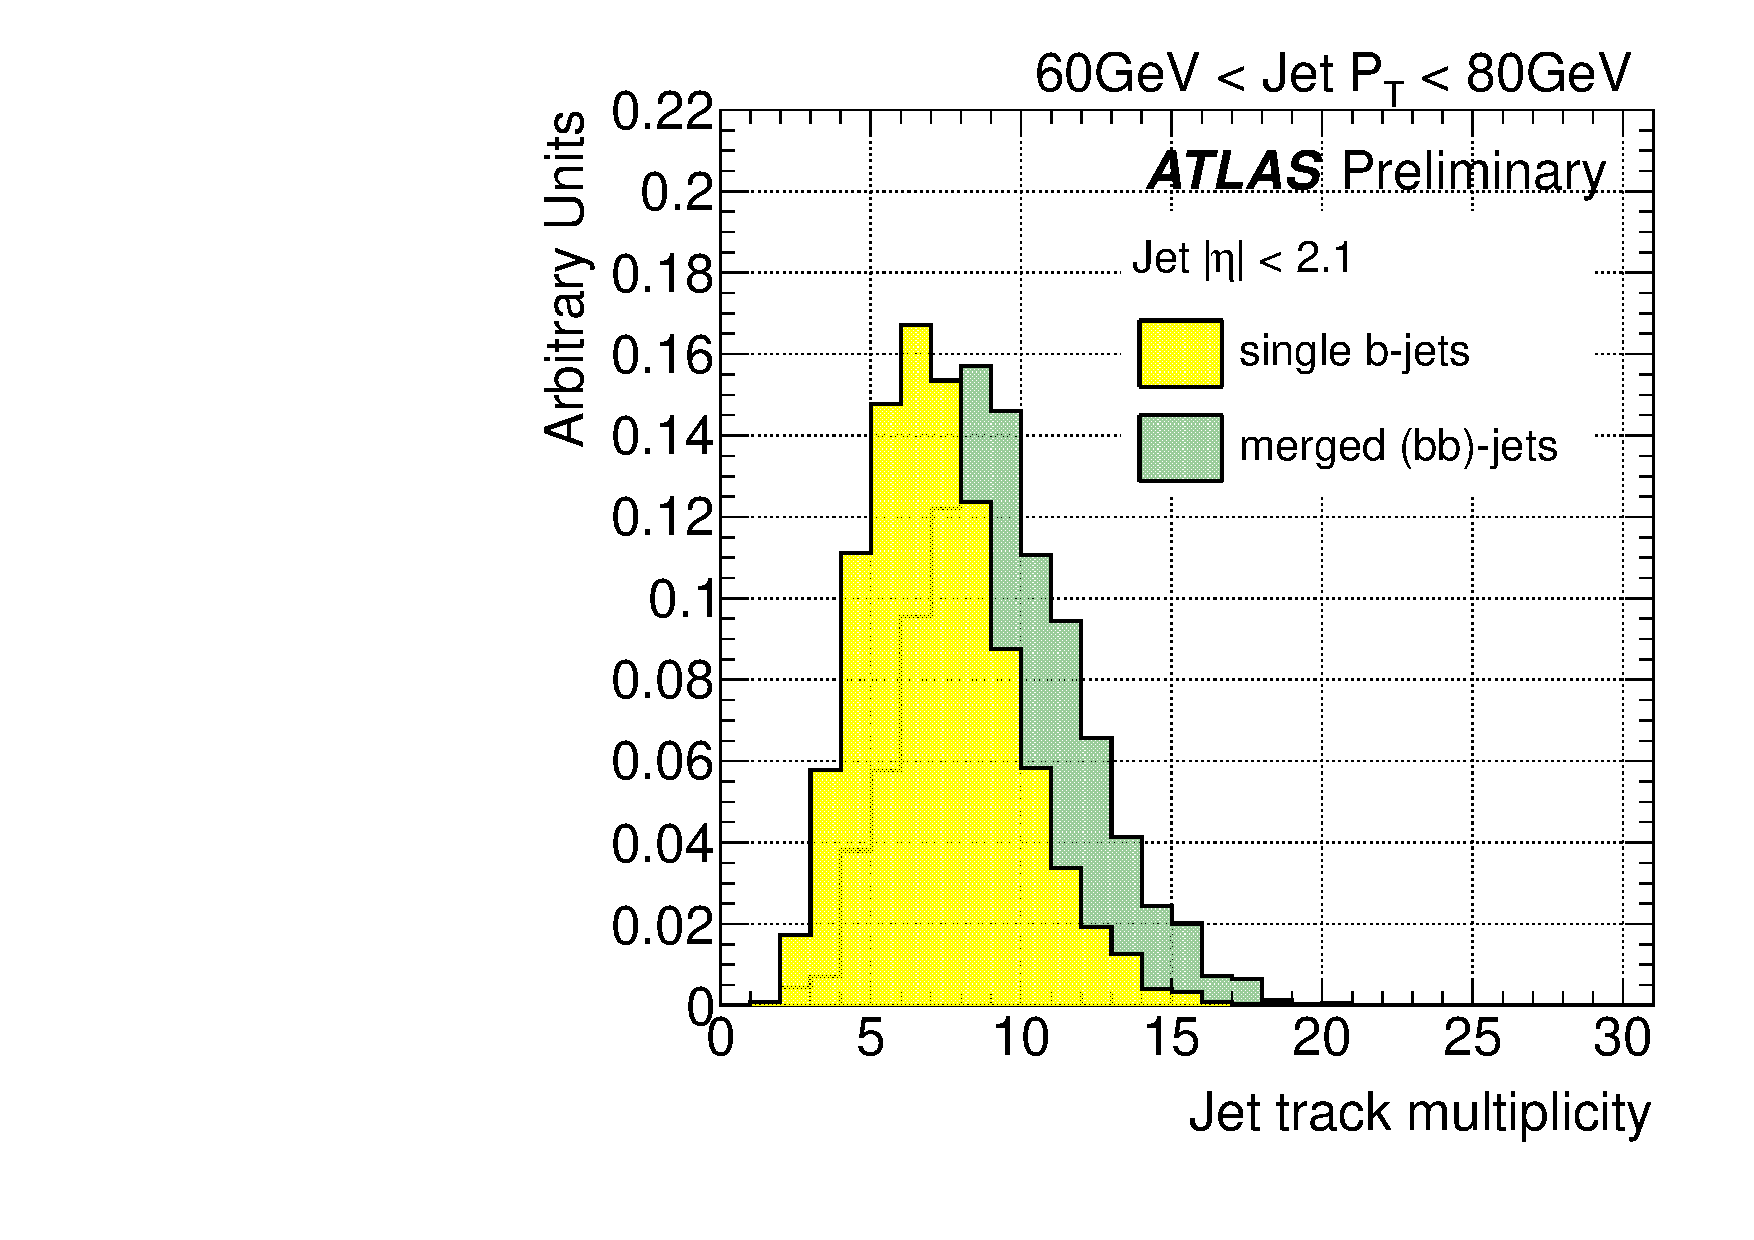
\includegraphics[width=0.49\textwidth]{FIGS/VarsSingleMerged/Ntrk060.pdf}
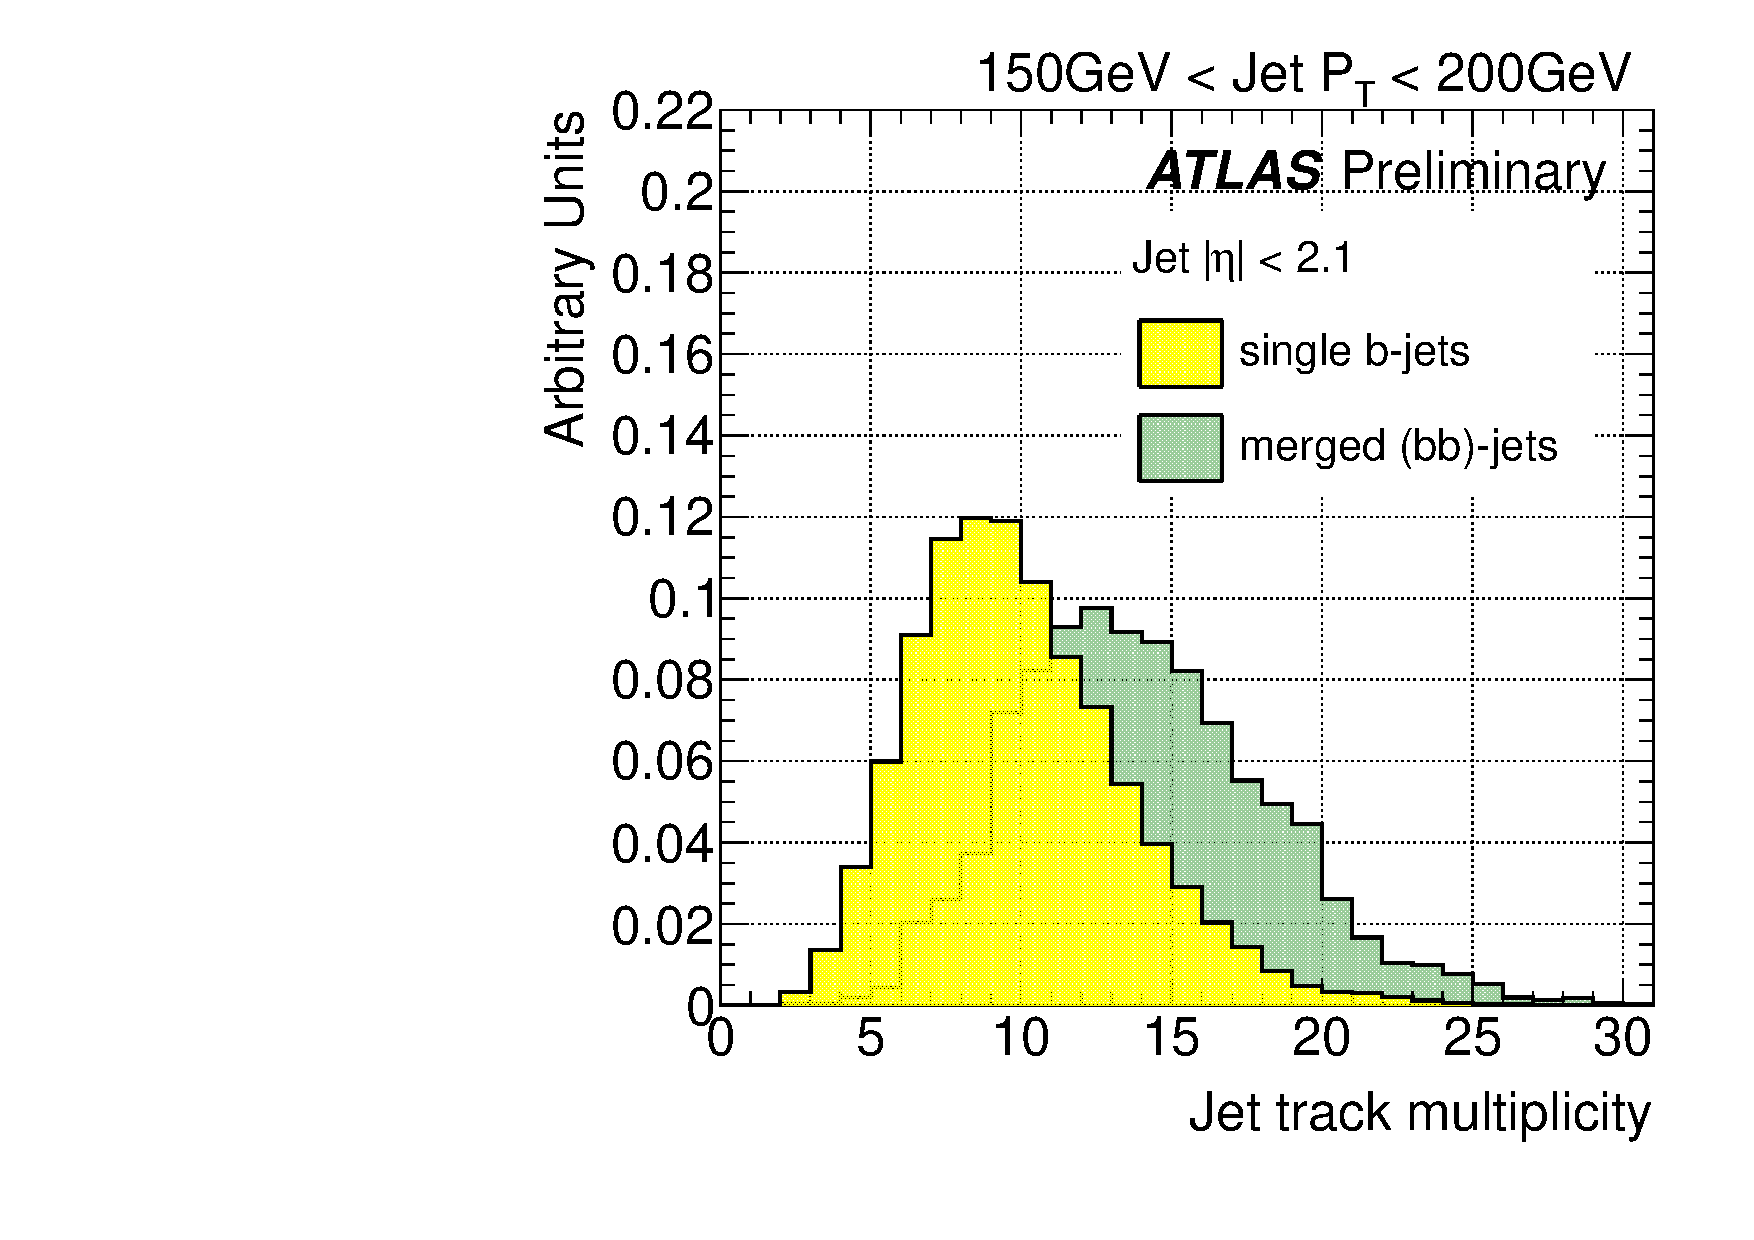
\includegraphics[width=0.49\textwidth]{FIGS/VarsSingleMerged/Ntrk150.pdf}
\caption{Distribution of track multiplicity in jets for single and merged $b$-jets between 60~GeV to 80~GeV (left) and 150~GeV to 200~GeV (right).}
\label{fig:ntrksinglemerged}
\end{figure}

\begin{figure}[tp]
\centering
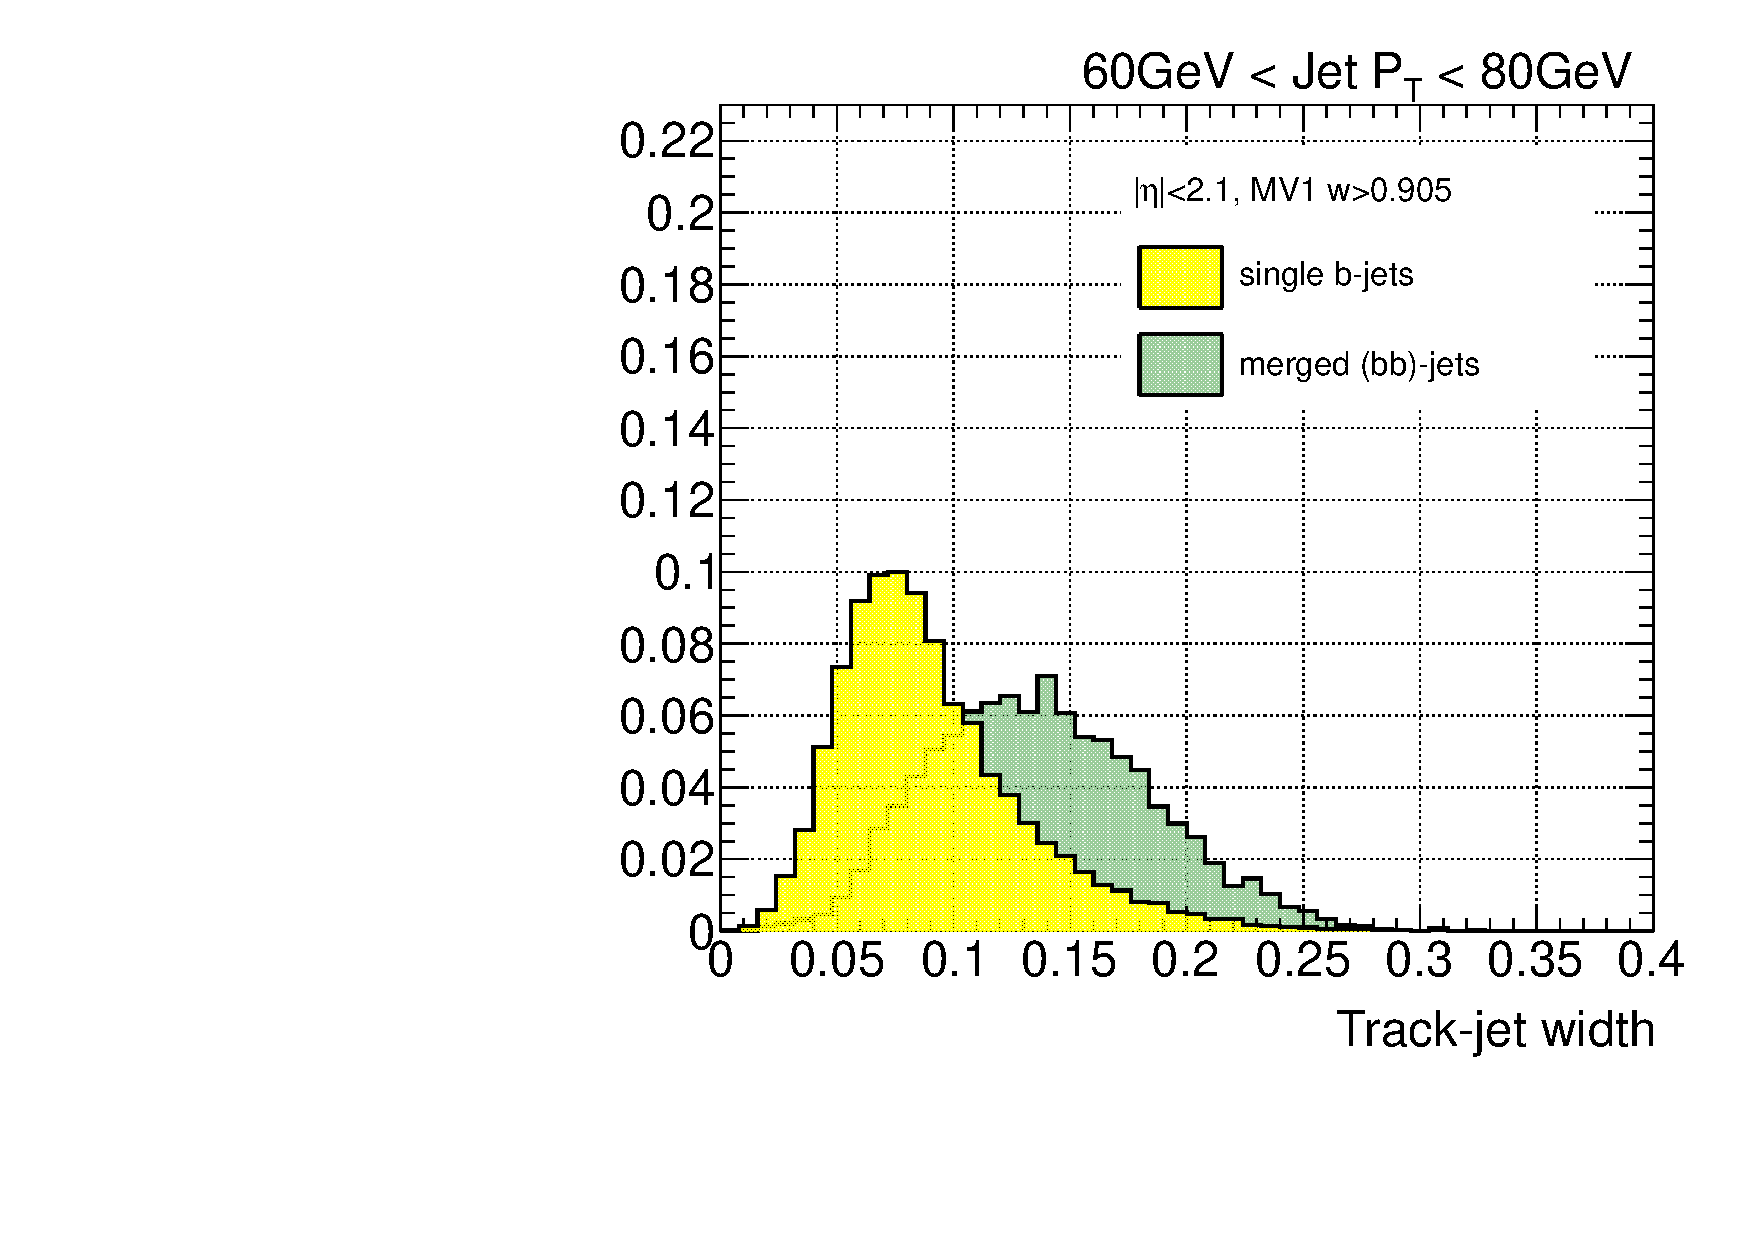
\includegraphics[width=0.49\textwidth]{FIGS/VarsSingleMerged/trkWidth060.pdf}
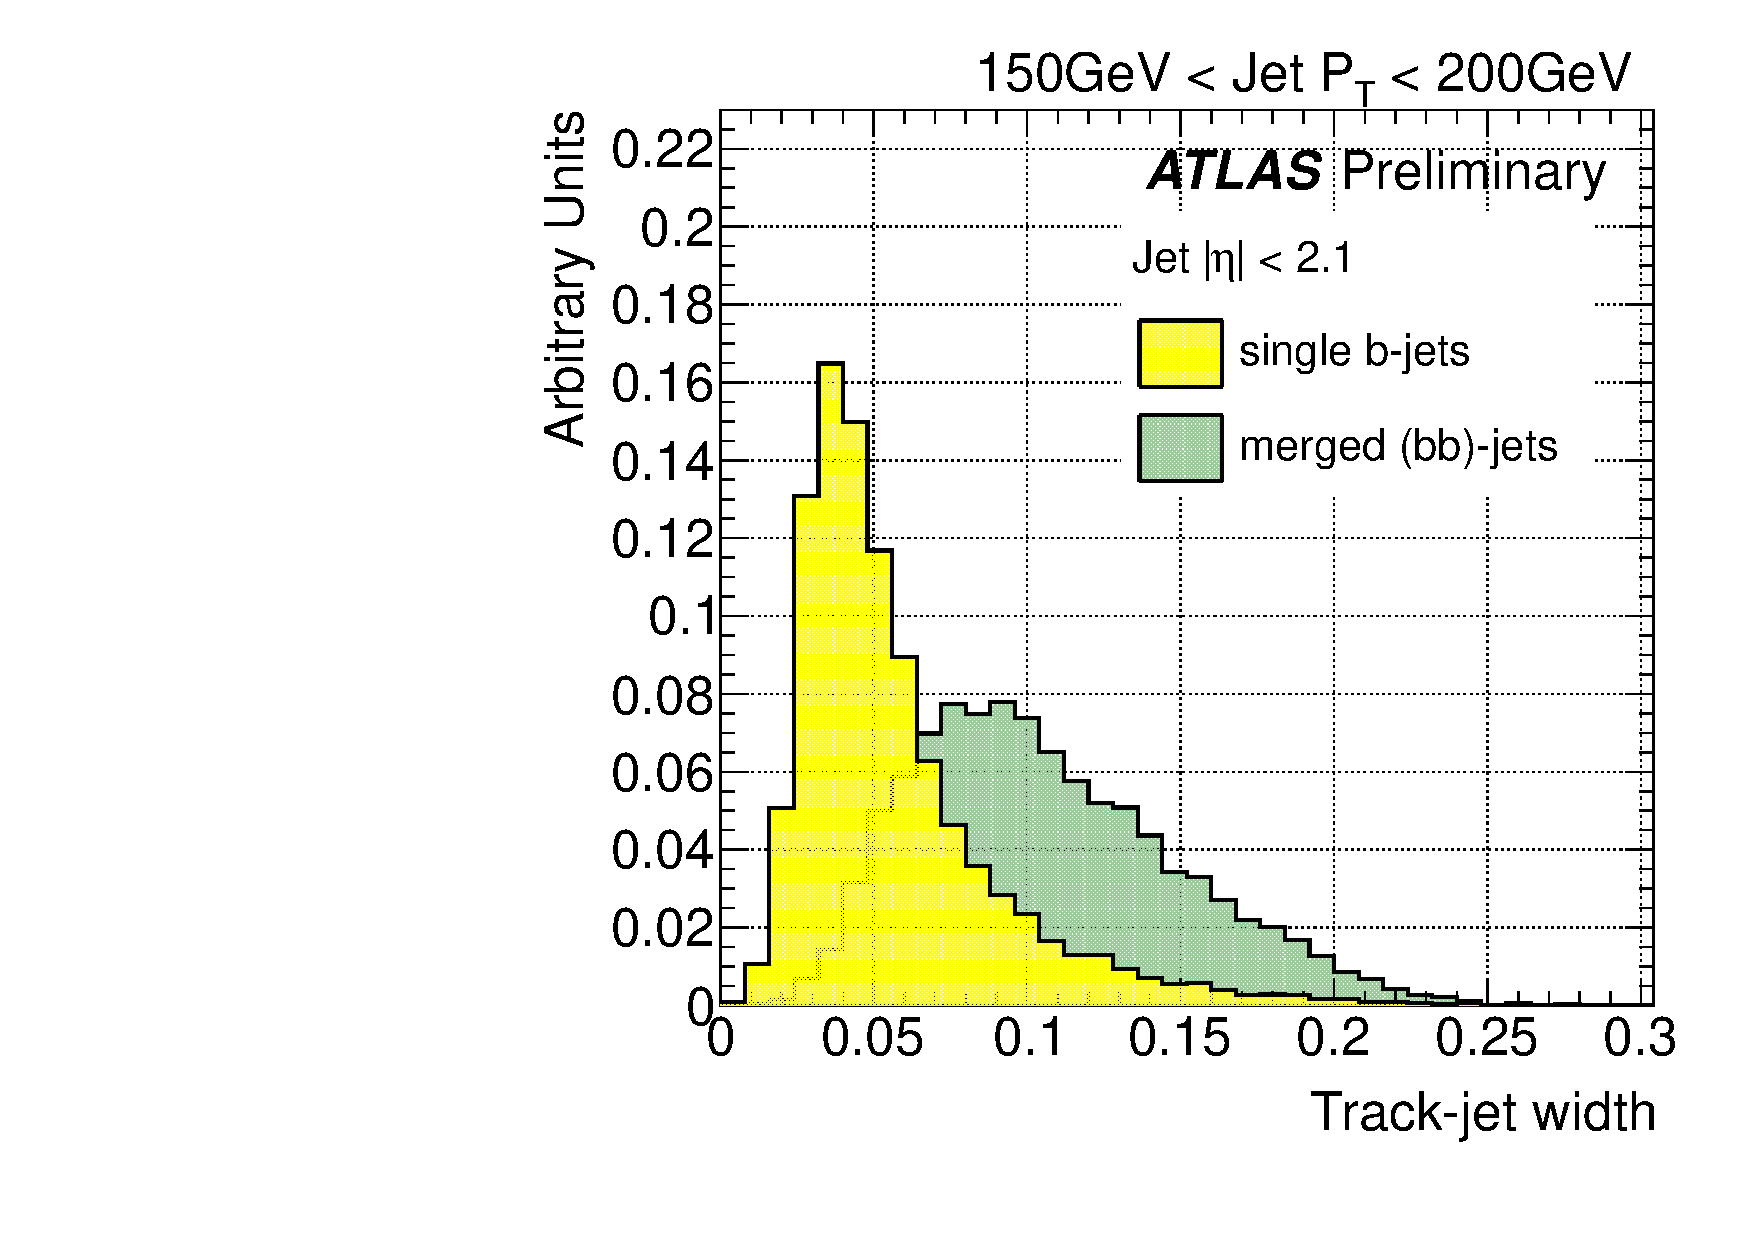
\includegraphics[width=0.49\textwidth]{FIGS/VarsSingleMerged/trkWidth150.pdf}
\caption{Distribution of track-jet width in jets for single and merged $b$-jets between 60~GeV to 80~GeV (left) and 150~GeV to 200~GeV (right).}
\label{fig:trkwidthsinglemerged}
\end{figure}


\begin{figure}[tp]
\centering
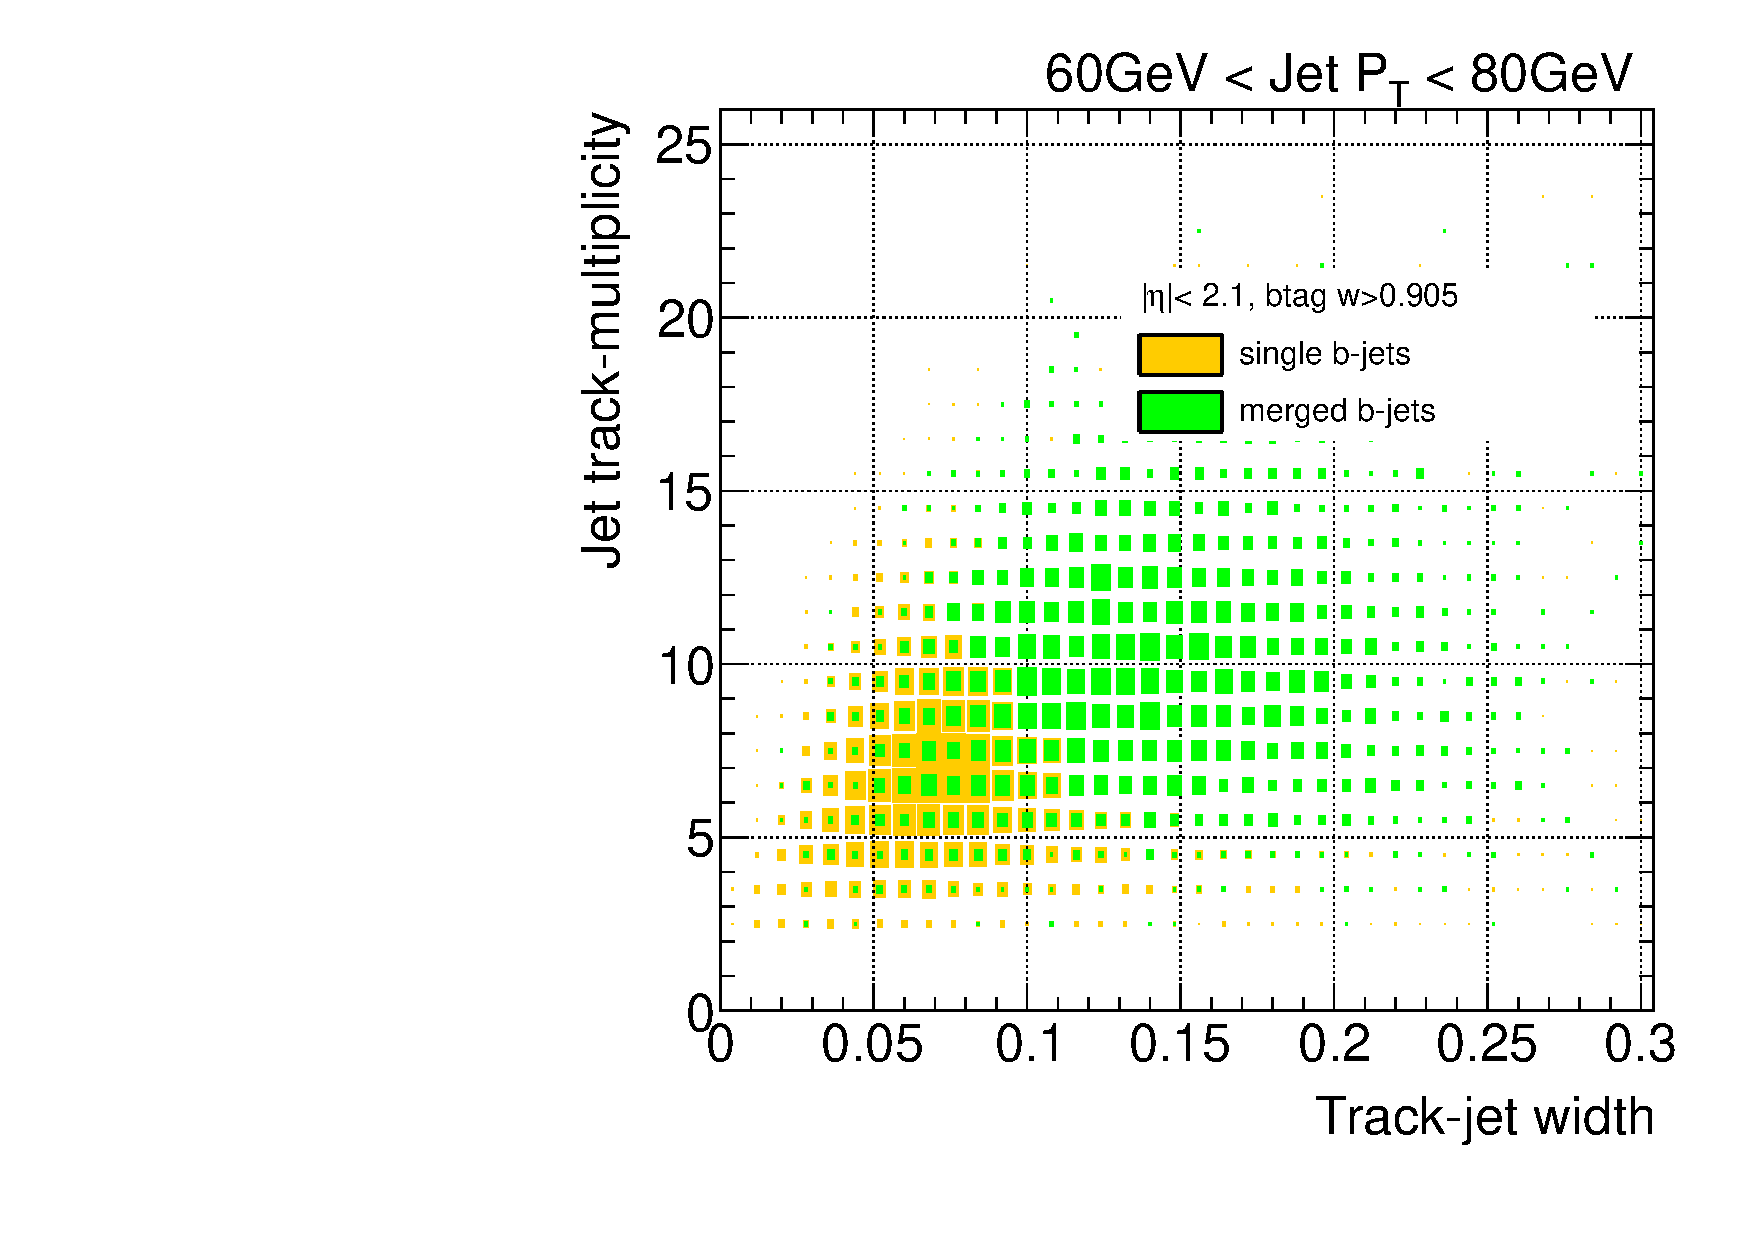
\includegraphics[width=0.49\textwidth]{FIGS/VarsSingleMerged/NtrktrkWidth060.pdf}
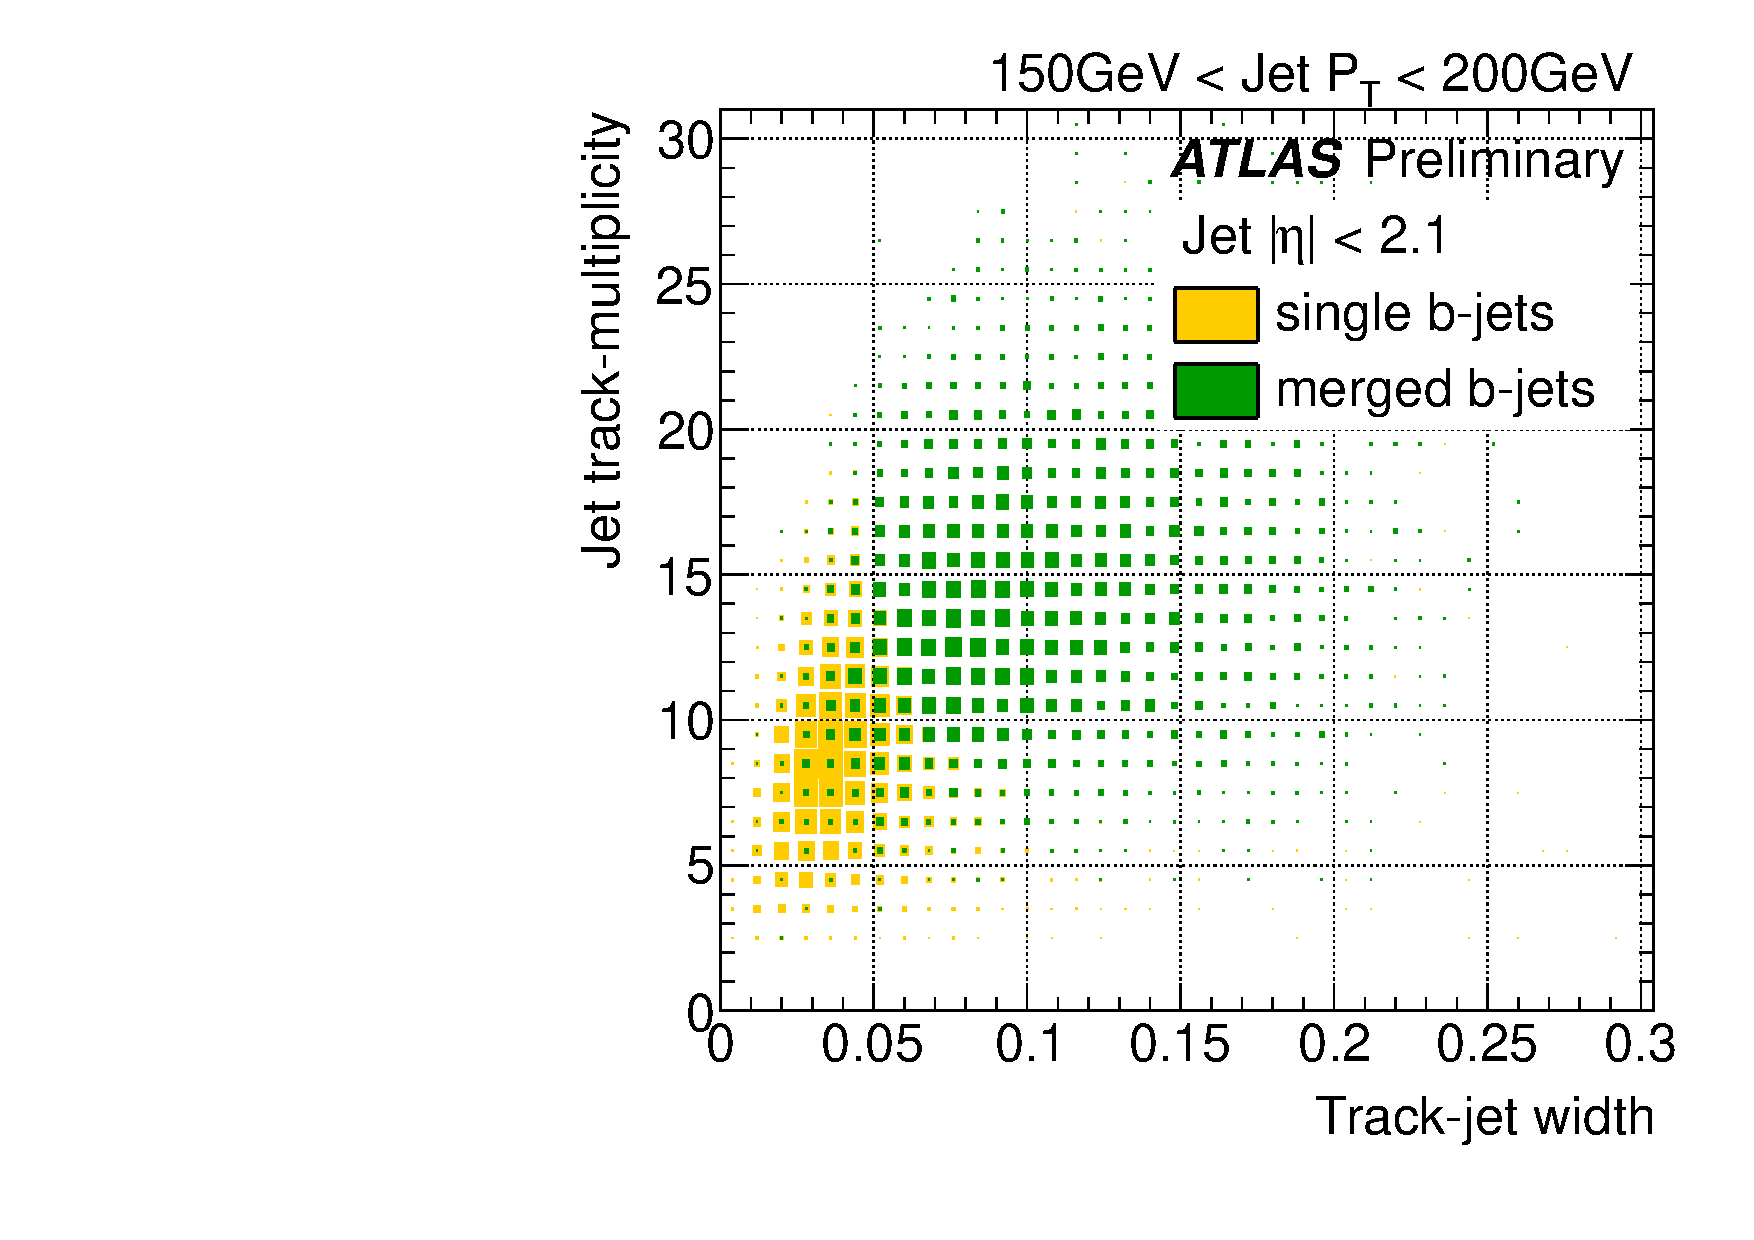
\includegraphics[width=0.49\textwidth]{FIGS/VarsSingleMerged/NtrktrkWidth150.pdf}
\caption{Correlation between track-multiplicity and track-jet width for single and merged $b$-jets between 60~GeV to 80~GeV (left) and 150~GeV to 200~GeV (right).}
\label{fig:ntrktrkwidthsinglemerged}
\end{figure}



\begin{figure}[tp]
\centering
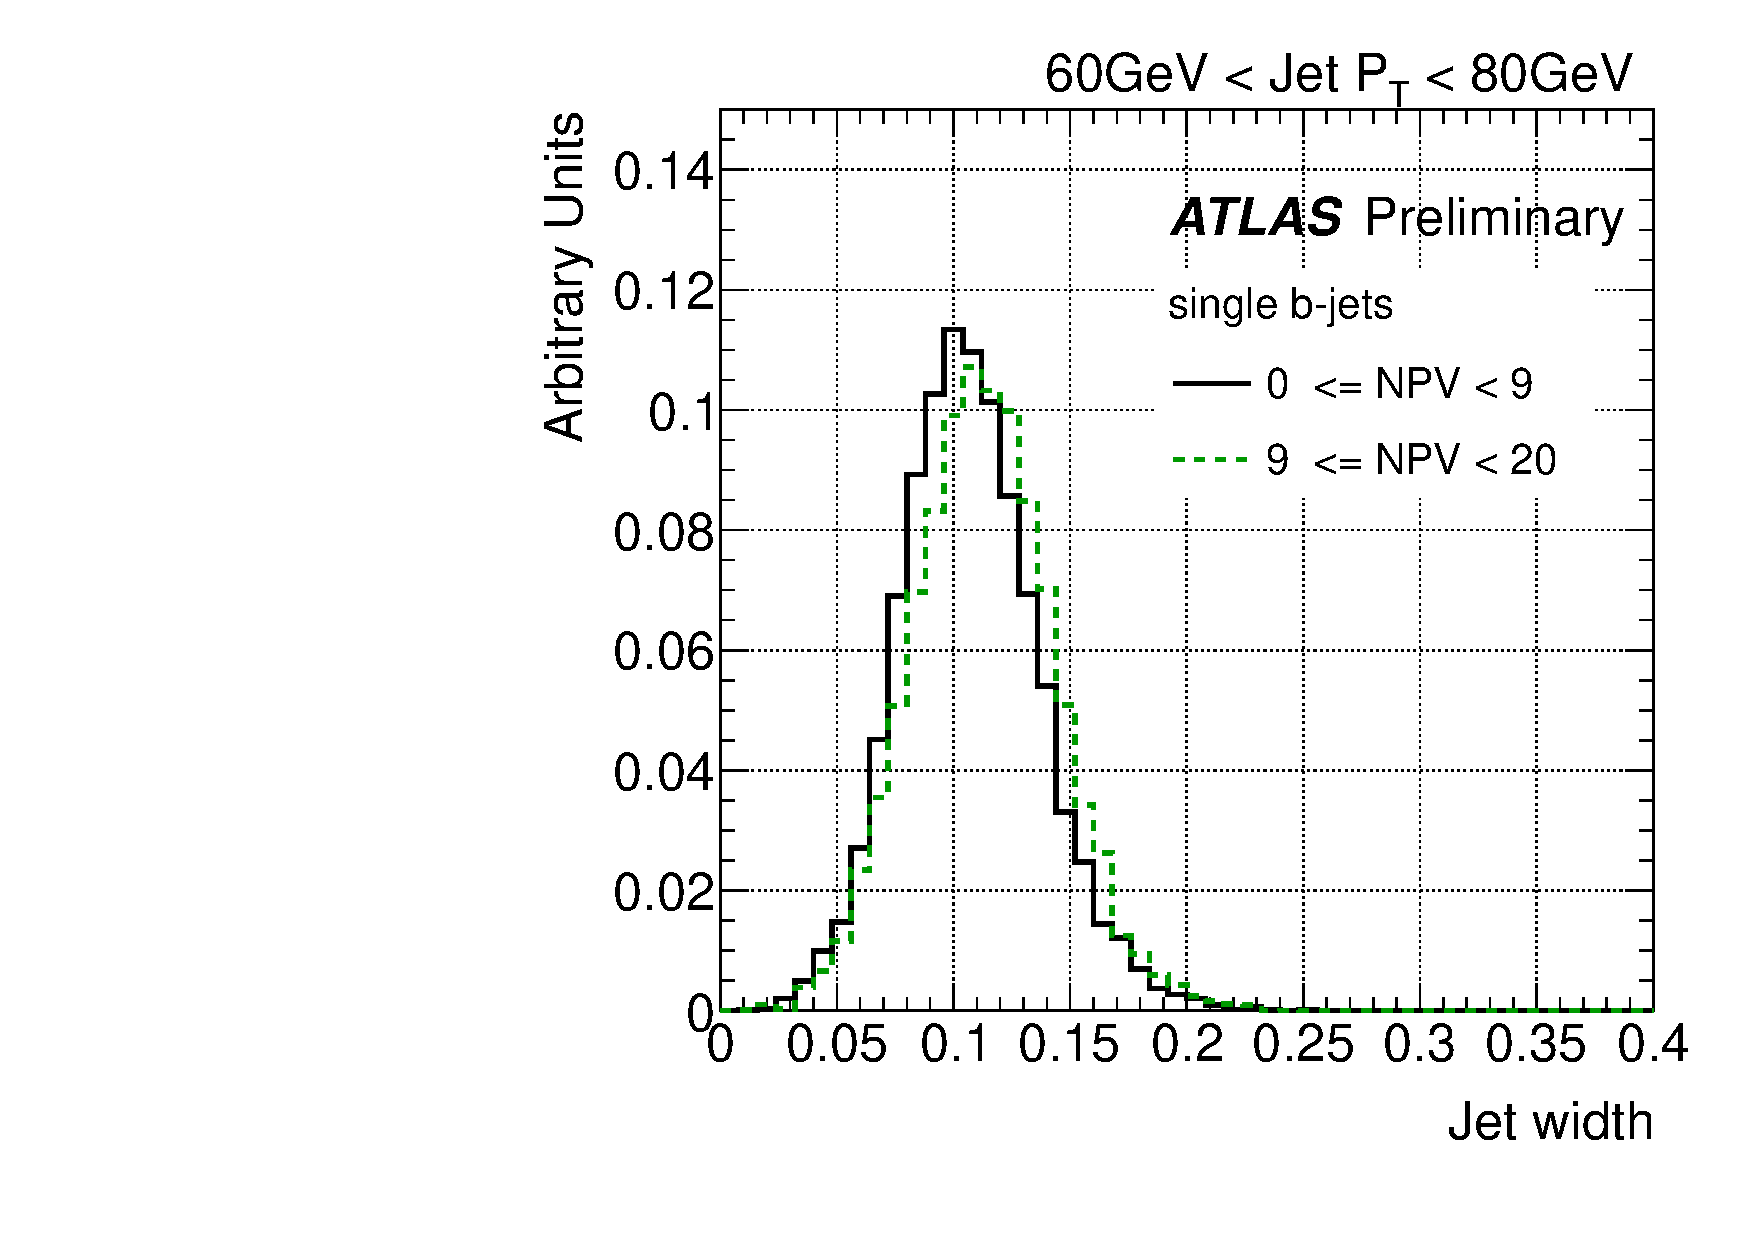
\includegraphics[width=0.49\textwidth]{FIGS/systematics/Widthsingle_060.pdf}
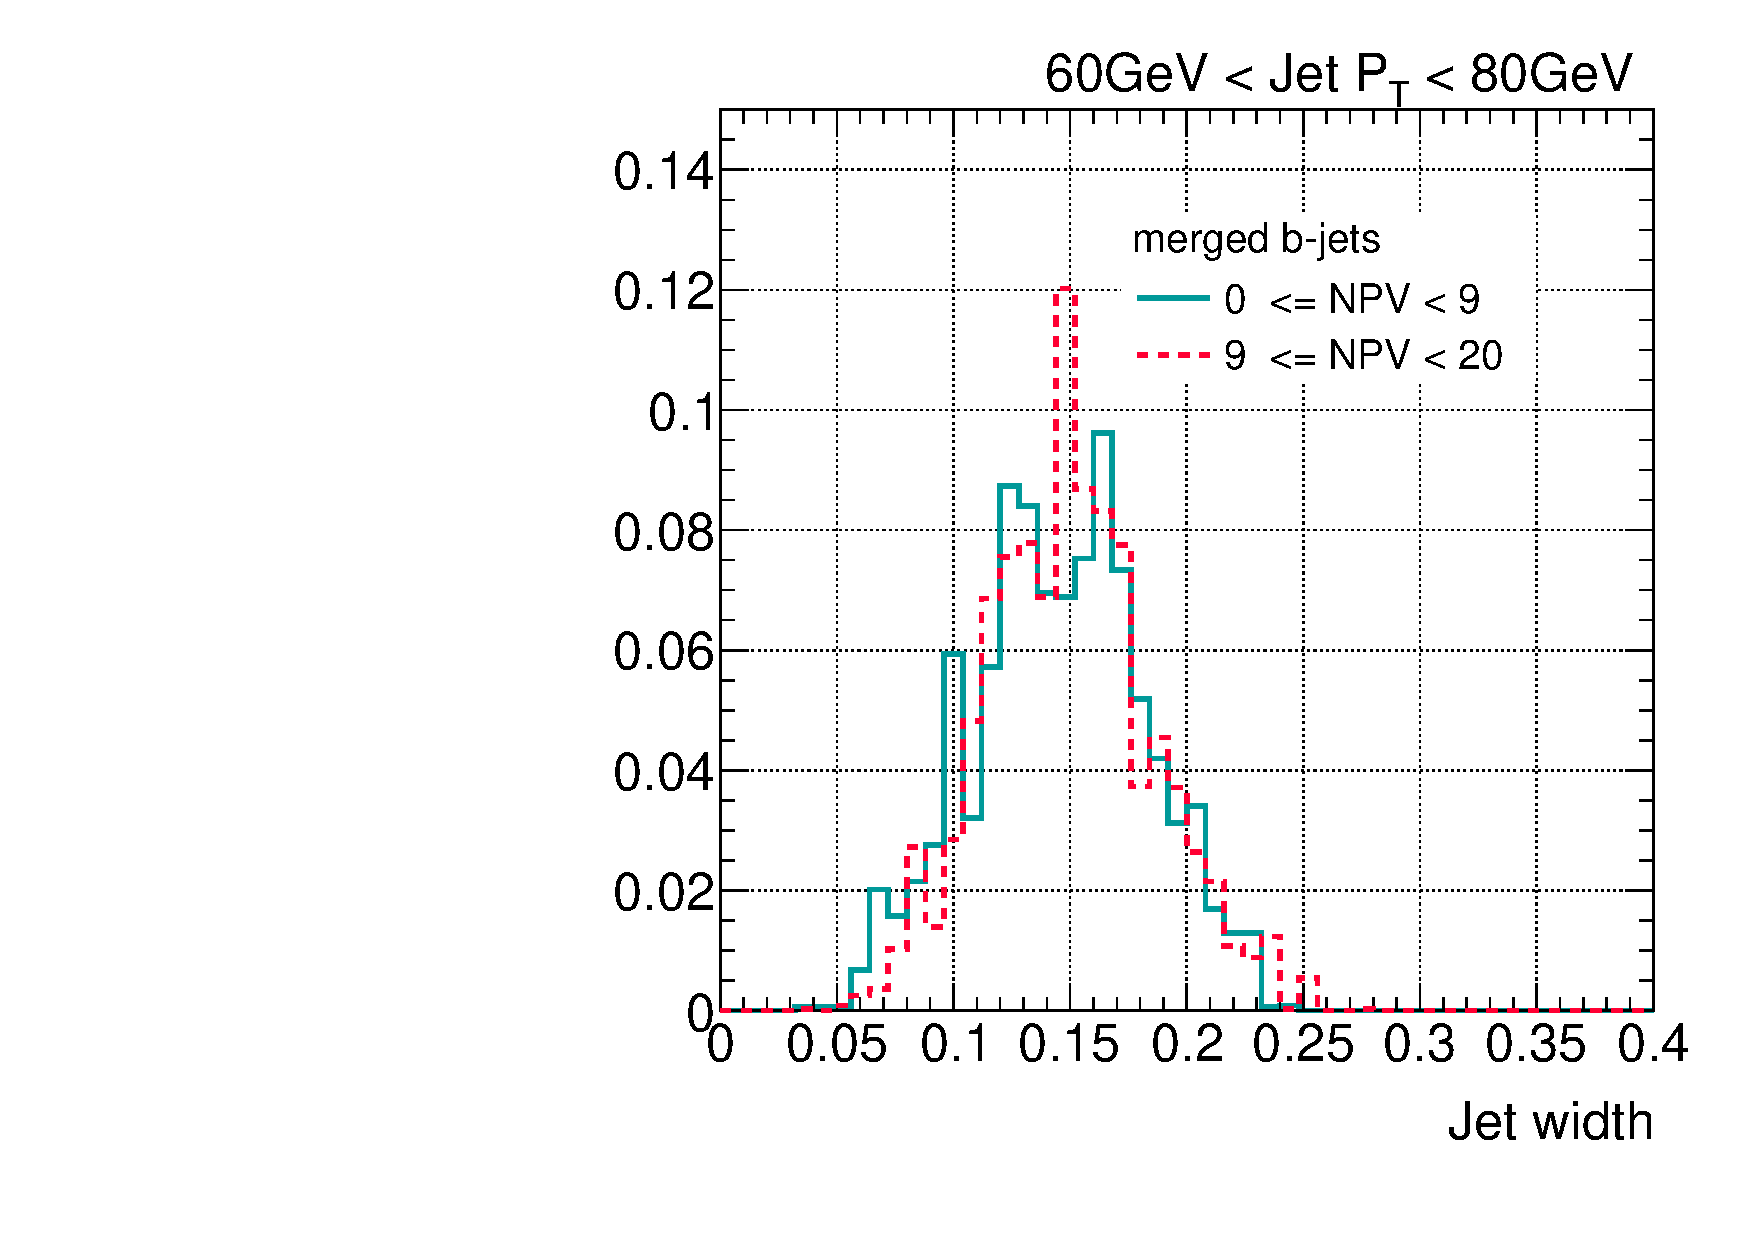
\includegraphics[width=0.49\textwidth]{FIGS/systematics/Widthmerged_060.pdf}
\caption{Distribution of calorimeter jet width for single (left) and merged (right) $b$-jets in bins of the Number of Primary Vertices for jets between 60~GeV to 80~GeV.}
\label{fig:calowidthpileup}
\end{figure}
systematics.ods

\begin{figure}[tp]
\centering
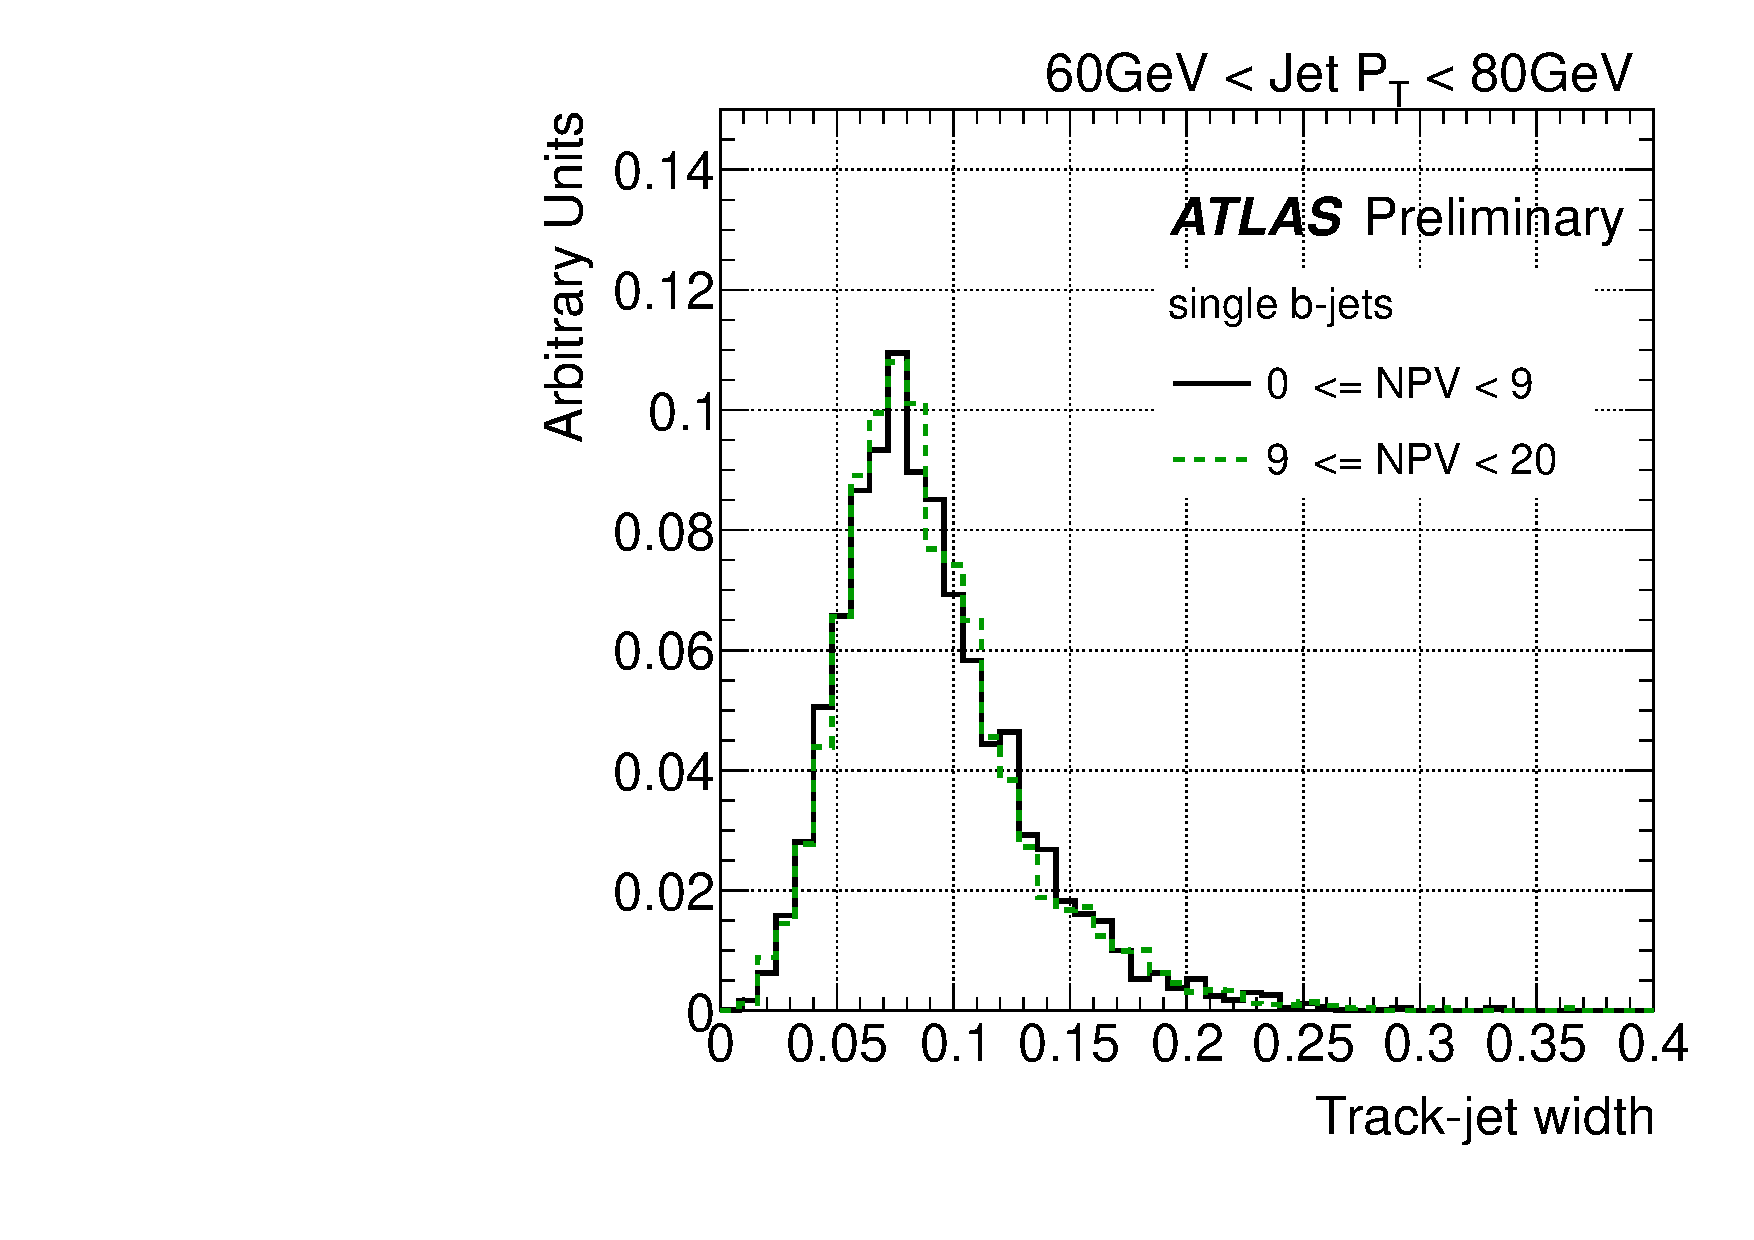
\includegraphics[width=0.49\textwidth]{FIGS/systematics/trkWidthsingle_060.pdf}
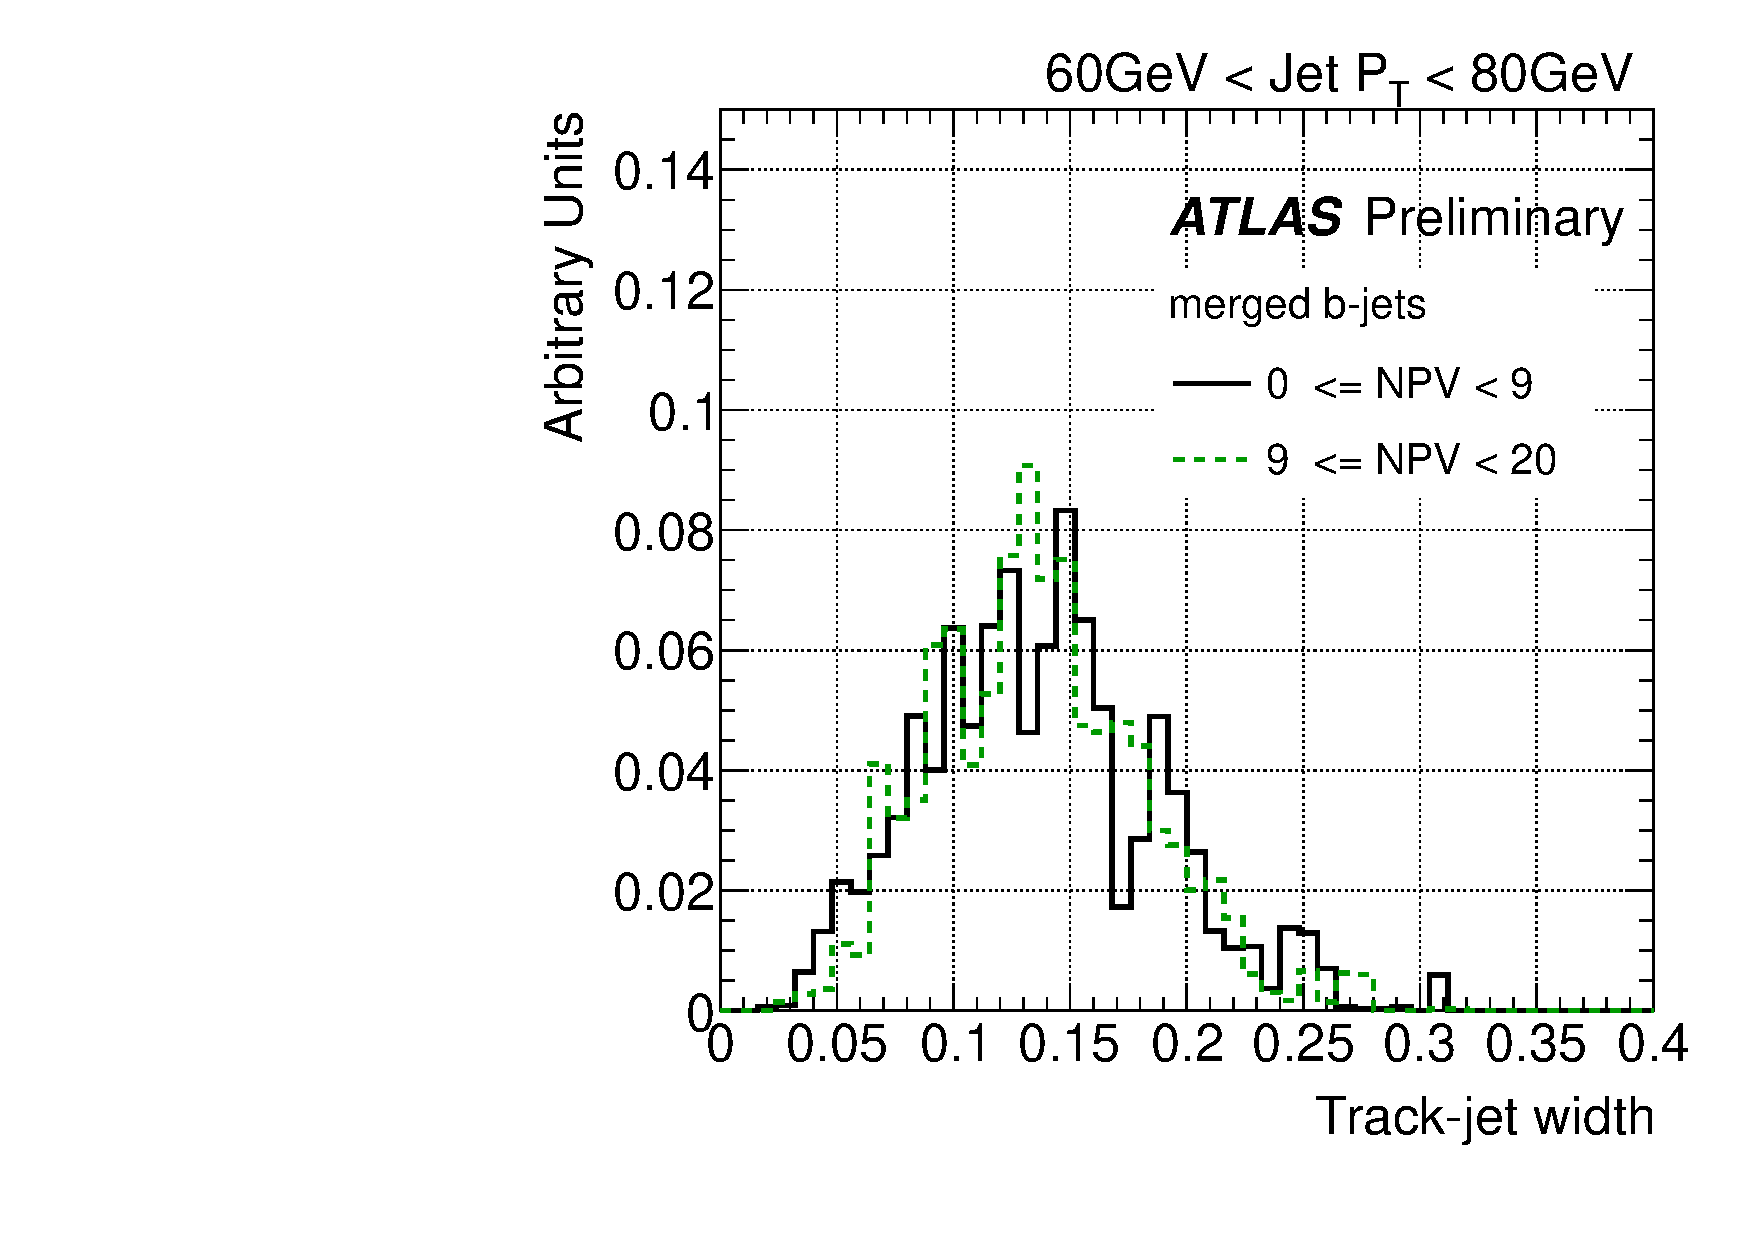
\includegraphics[width=0.49\textwidth]{FIGS/systematics/trkWidthmerged_060.pdf}
\caption{Distribution of track-jet width for single (left) and merged (right) $b$-jets in bins of the Number of Primary Vertices for jets between 60~GeV to 80~GeV.}
\label{fig:trkwidthpileup}
\end{figure}


Figure~\ref{fig:drmaxsinglemerged} shows the distribution of the maximum $\Delta R$ between track pairs in the jets ($\Delta R_{\rm max}$). Merged $b$-jets show significantly higher values for this variable over a broad range of jet $\pt$. The distinct characteristic of this variable is that the separation between single $b$-jets and merged does not depend on jet $\pt$. In spite of its good discrimination power, we have looked for alternatives to $\Delta R_{\rm max}$ as it is not an infrared safe magnitude and is sensitive to soft tracks originating from pile-up. 

The distribution of the $\Delta R$ between the axis of the two $k_t$-subjets in the jet is shown in Fig.~\ref{fig:drktsinglemerged} for single and merged $b$-jets. For this variable, tracks inside the jets are clustered into exactly two subjets using the $k_t$ jet algorithm implemented in fastjet~\cite{fastjet}. We observe that it also provides good separation, with the advantage of infrared safeness and insensitivity to pile-up. % revealing the two-prong substructure of merged $b$-jets.

$N$-subjettiness variables, as described in Ref.~\cite{nsubjettiness}, were originally designed to identify boosted objects, like electroweak bosons and top quarks, decaying into collimated shower of hadrons which a standard jet algorithm would reconstruct as single jets. It is defined as:
\begin{equation*} 
\tau_N = \frac{1}{\sum_k {\pt}_k\,R_0} \sum_k {\pt}_k \min \{ \Delta R_{S_1,k},\,\Delta R_{S_2,k},...,\,\Delta R_{S_N,k} \}
\end{equation*} 
where $R_0$ is the jet radius used in the jet clustering algorithm and the sum runs over the components of the jet. To avoid dependence on pile-up we consider the track-based subjettiness, where the sum 
 is over the tracks in the $b$-tagged jet. $\Delta R_{S_j,k} $ is the distance in the rapidity-azimuth plane between the axis of subjet $j$ and constituent track $k$. This jet shape variable quantifies to what degree a jet can be regarded as composed of $N$ subjets. For instance, a jet with a two pronged structure, with all tracks clustered along two directions, is expected to have a smaller $\tau_2$ value than a jet with tracks uniformly distributed in $\eta-\phi$ space.

Plots of $ \tau_2$ are shown in Fig.~\ref{fig:tau2singlemerged}. In spite of its expected 2-prong substructure, merged $b$-jets have higher values of $ \tau_2$ than single $b$-jets. The explanation of this behavior can be found in Fig.~\ref{fig:tau2trkwidthsinglemerged}, where its correlation with  track-width ($\tau_1$) is shown for single and merged $b$-jets. The two variables are highly correlated and for this reason wider jets  have a larger $ \tau_2$. This suggests to switch from an absolute to a width-normalized
$\tau_2$. Fig.~\ref{fig:tauratiosinglemerged} thus shows the distributions of $\tau_2/\tau_1$. Although as expected somewhat larger values are obtained for single than for merged $b$-jets, especially at high \pt, we decided not to use this variable as it offers only marginal discrimination. 

Variables such as the $\Delta R$ between the two leading tracks in jets and the jet eccentricity did not show good discrimination either and were not considered for the multivariate study.

\begin{figure}[tp]
\centering
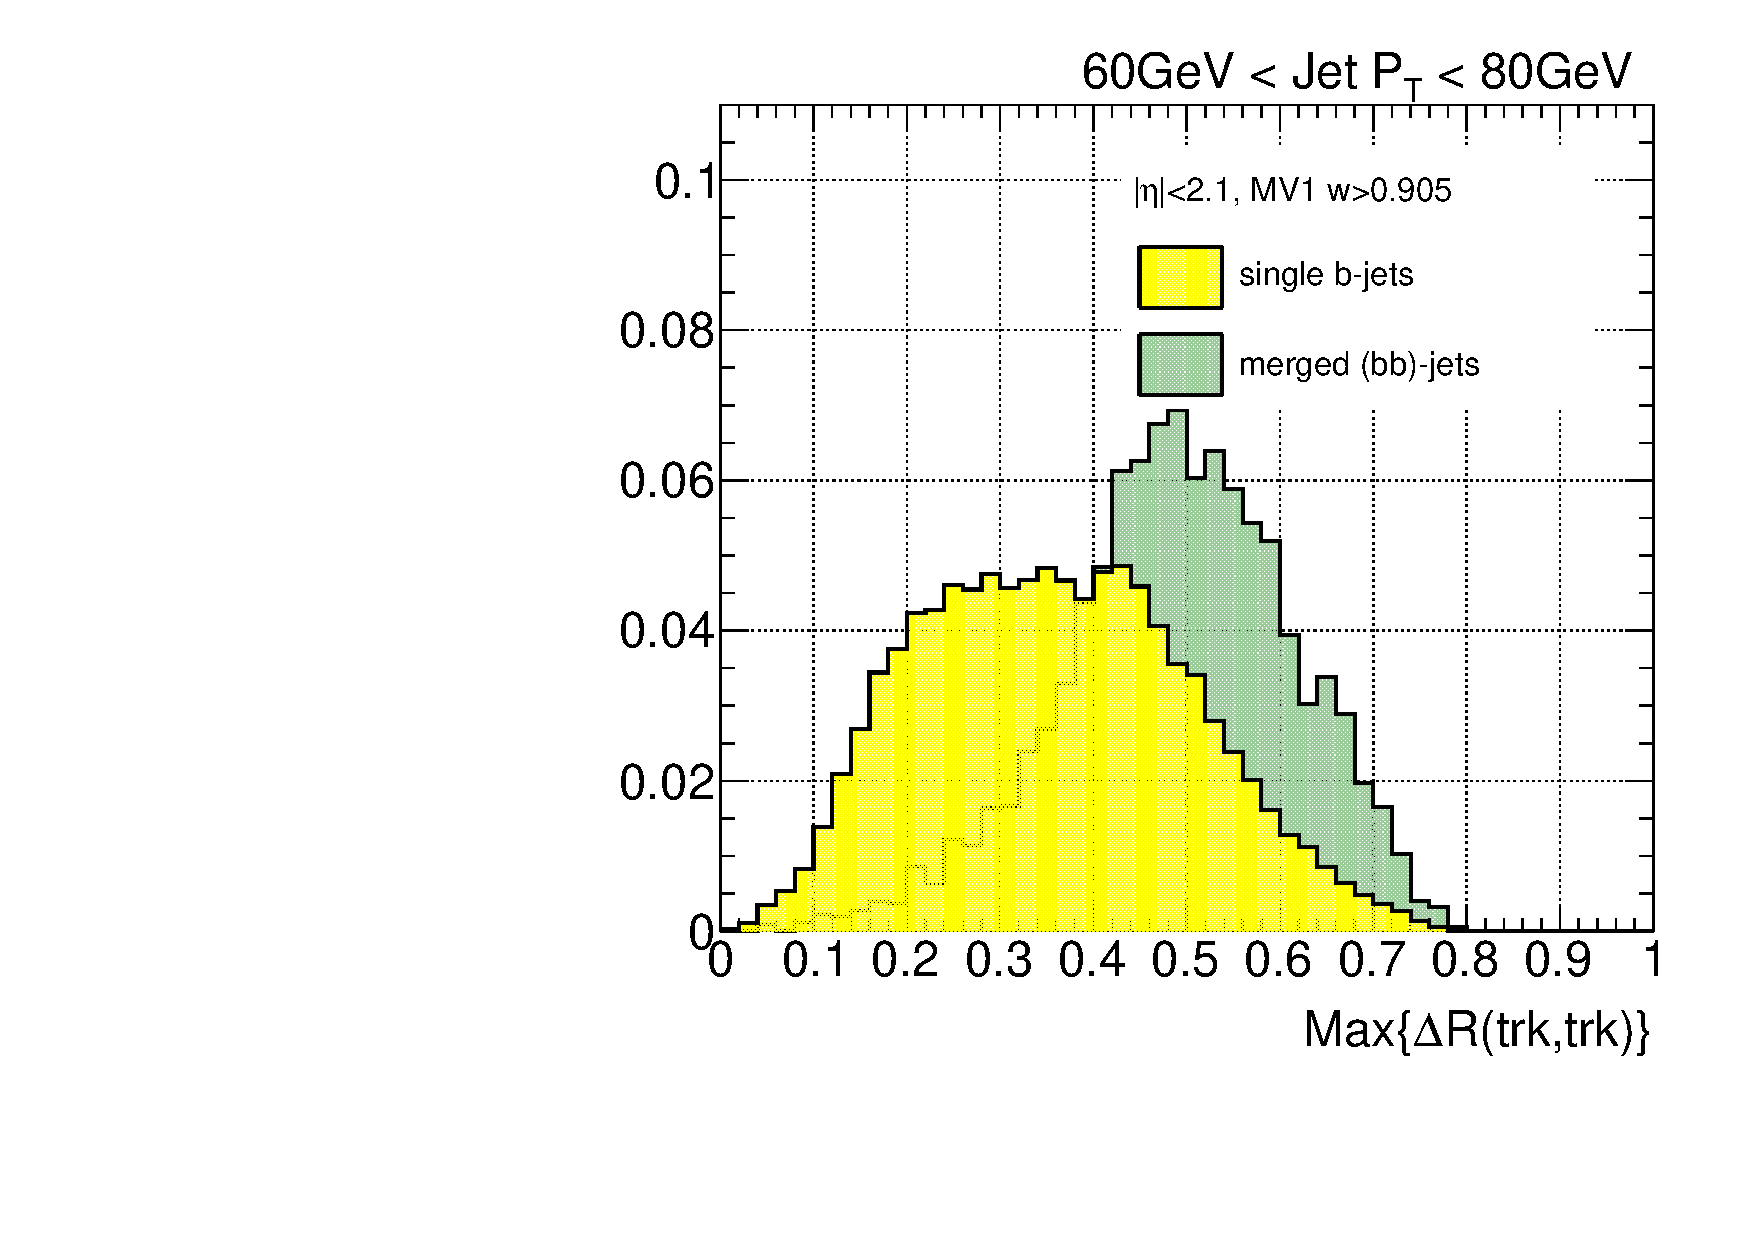
\includegraphics[width=0.49\textwidth]{FIGS/VarsSingleMerged/drmax060.pdf}
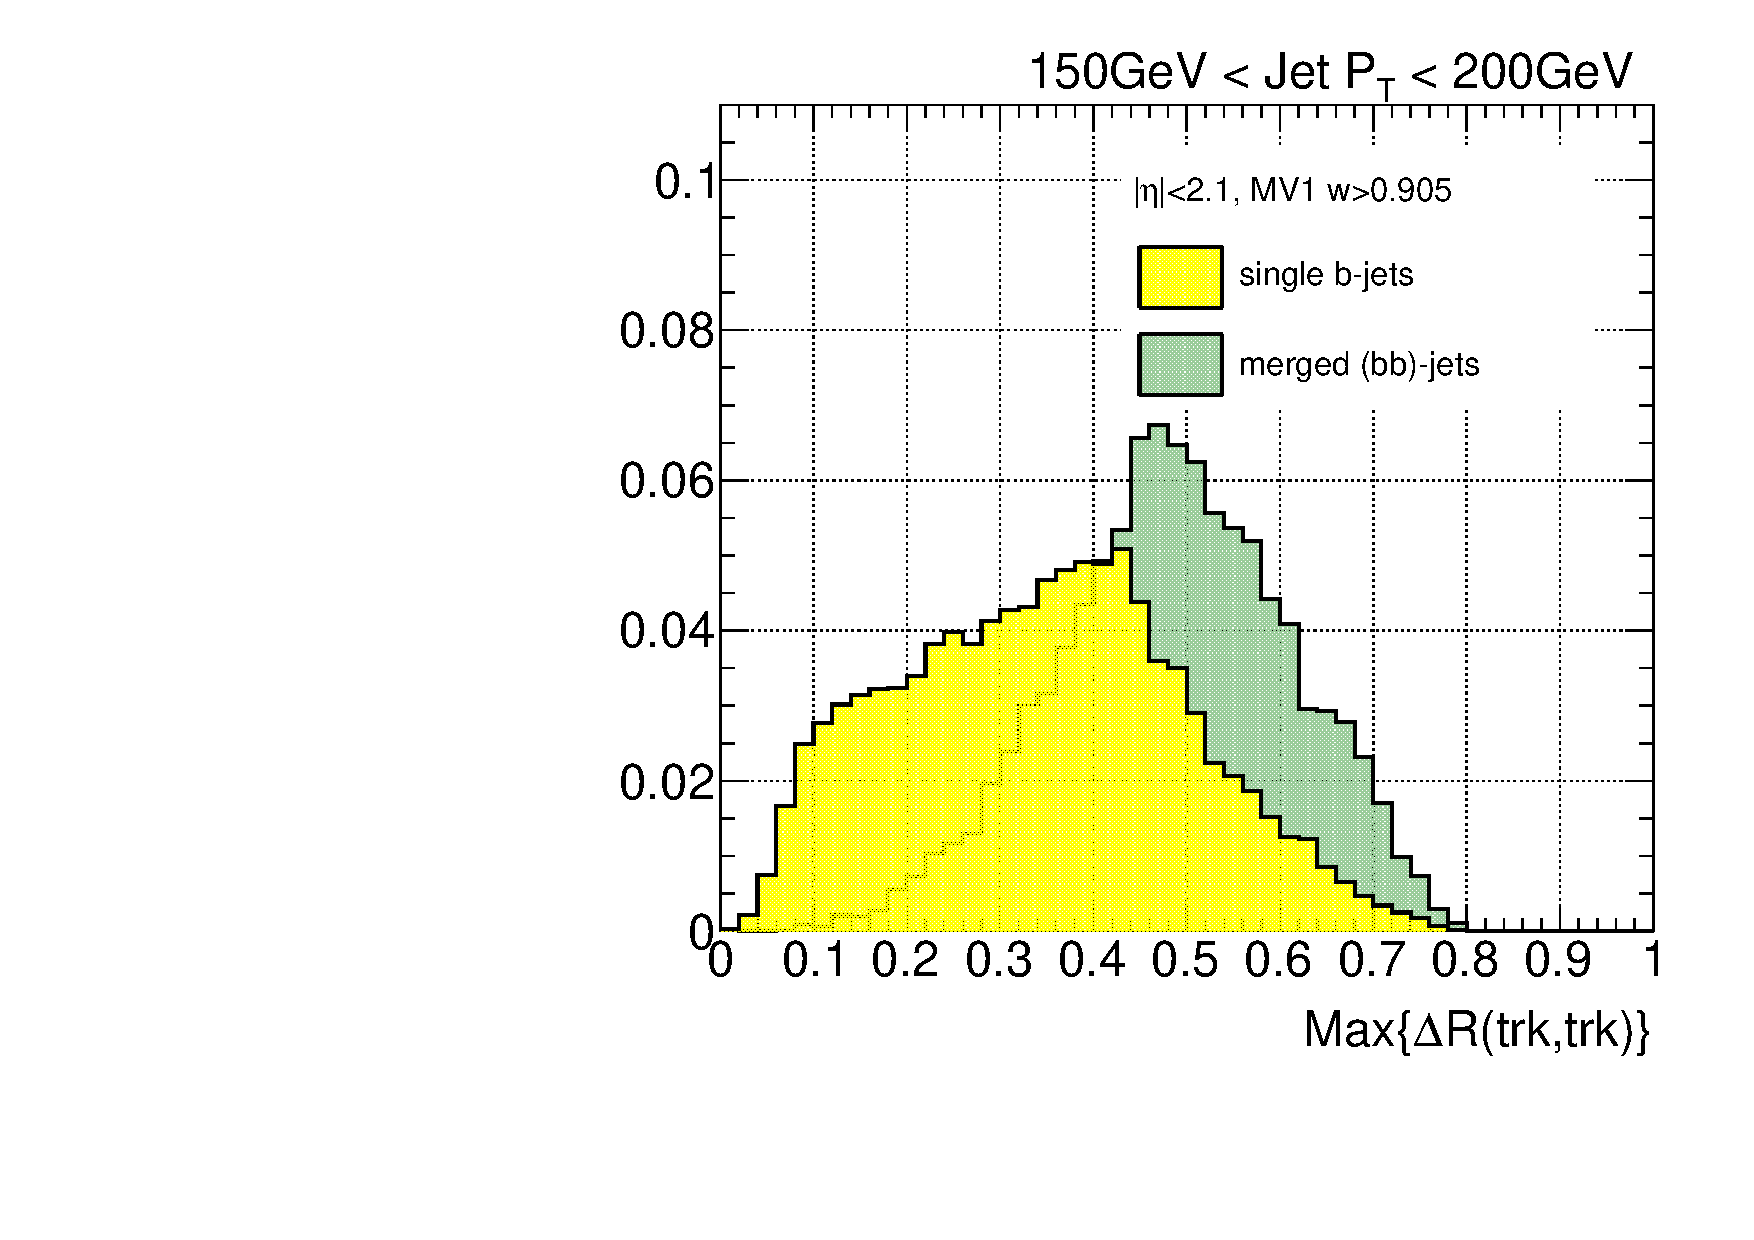
\includegraphics[width=0.49\textwidth]{FIGS/VarsSingleMerged/drmax150.pdf}
\caption{Distribution of the maximum $\Delta R$ between pairs in jets ($\Delta R_{\rm max}$) for single and merged $b$-jets between 60~GeV to 80~GeV (left) and 150~GeV to 200~GeV (right).}
\label{fig:drmaxsinglemerged}
\end{figure}

\begin{figure}[tp]
\centering
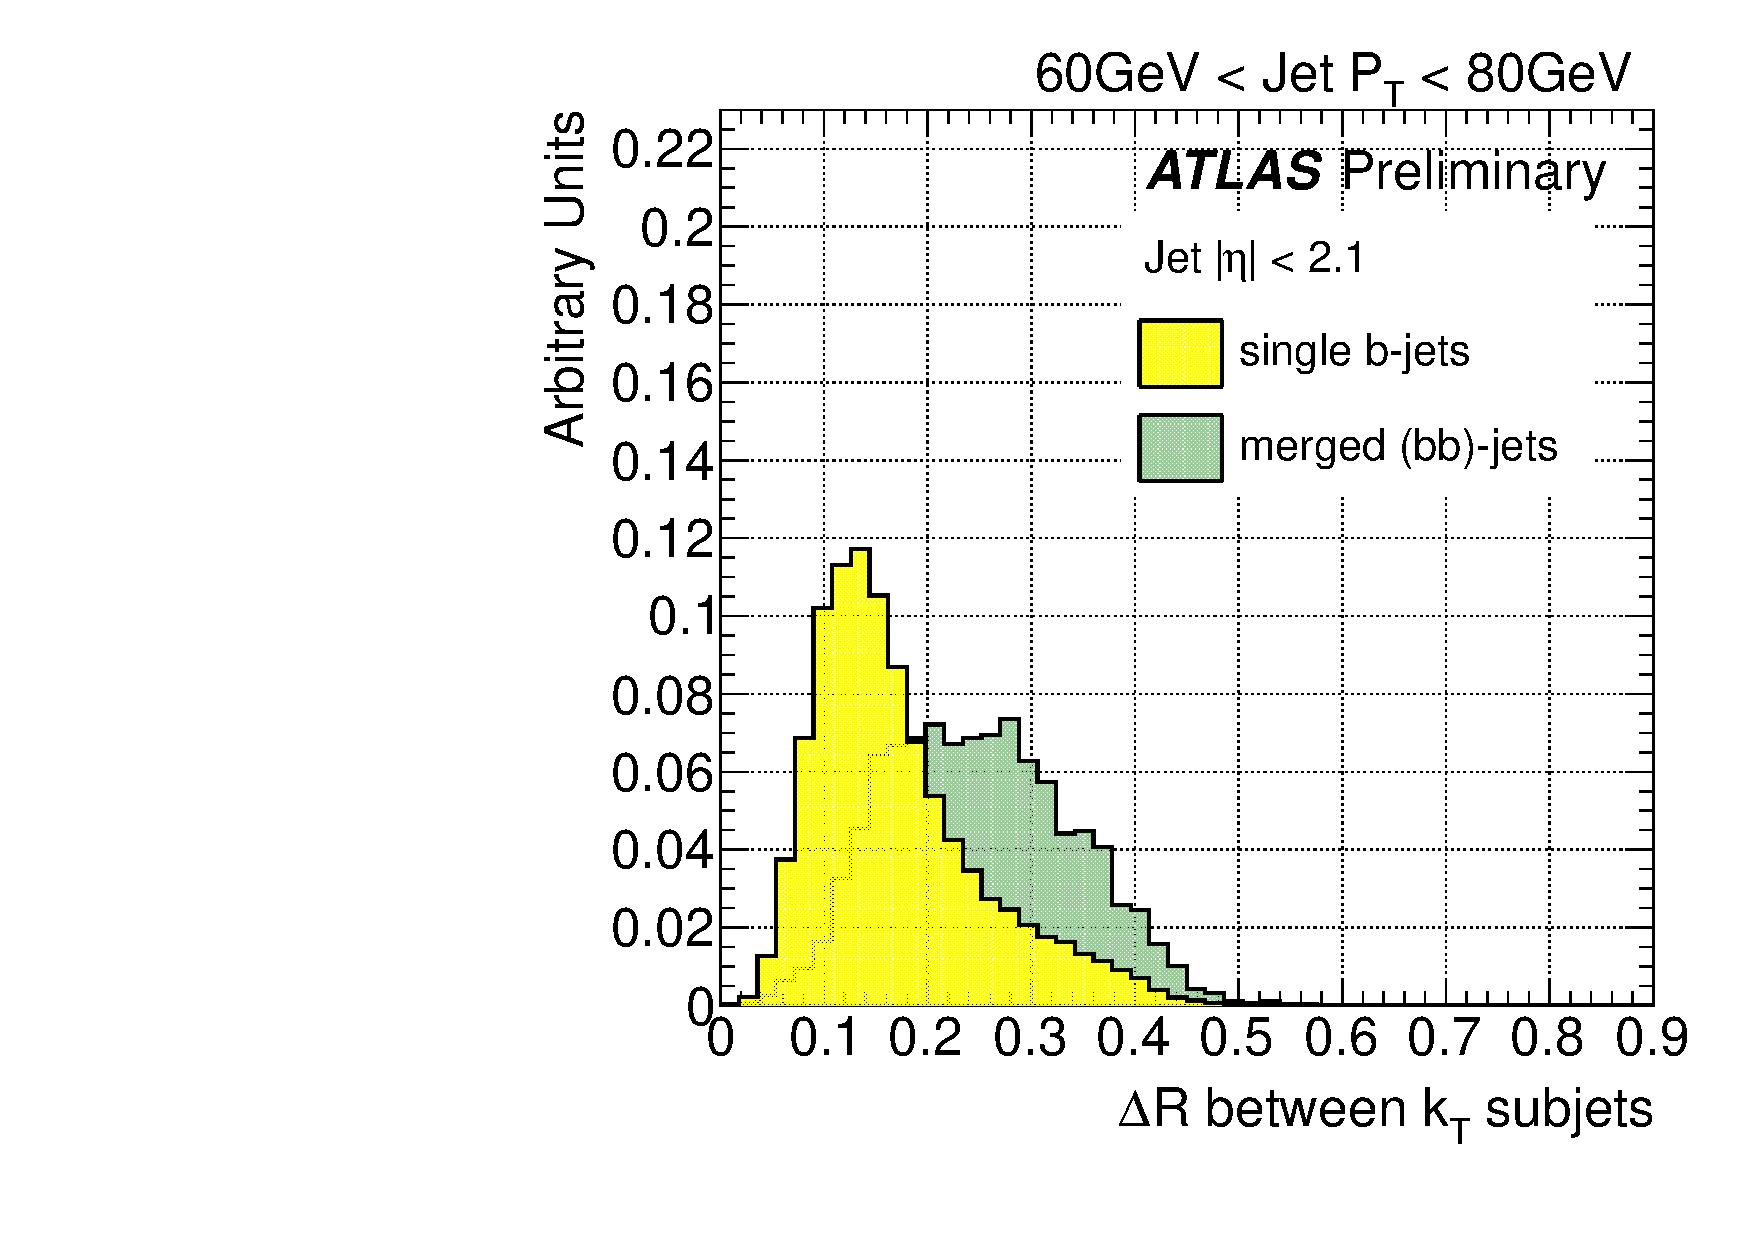
\includegraphics[width=0.49\textwidth]{FIGS/VarsSingleMerged/DRkt2axes060.pdf}
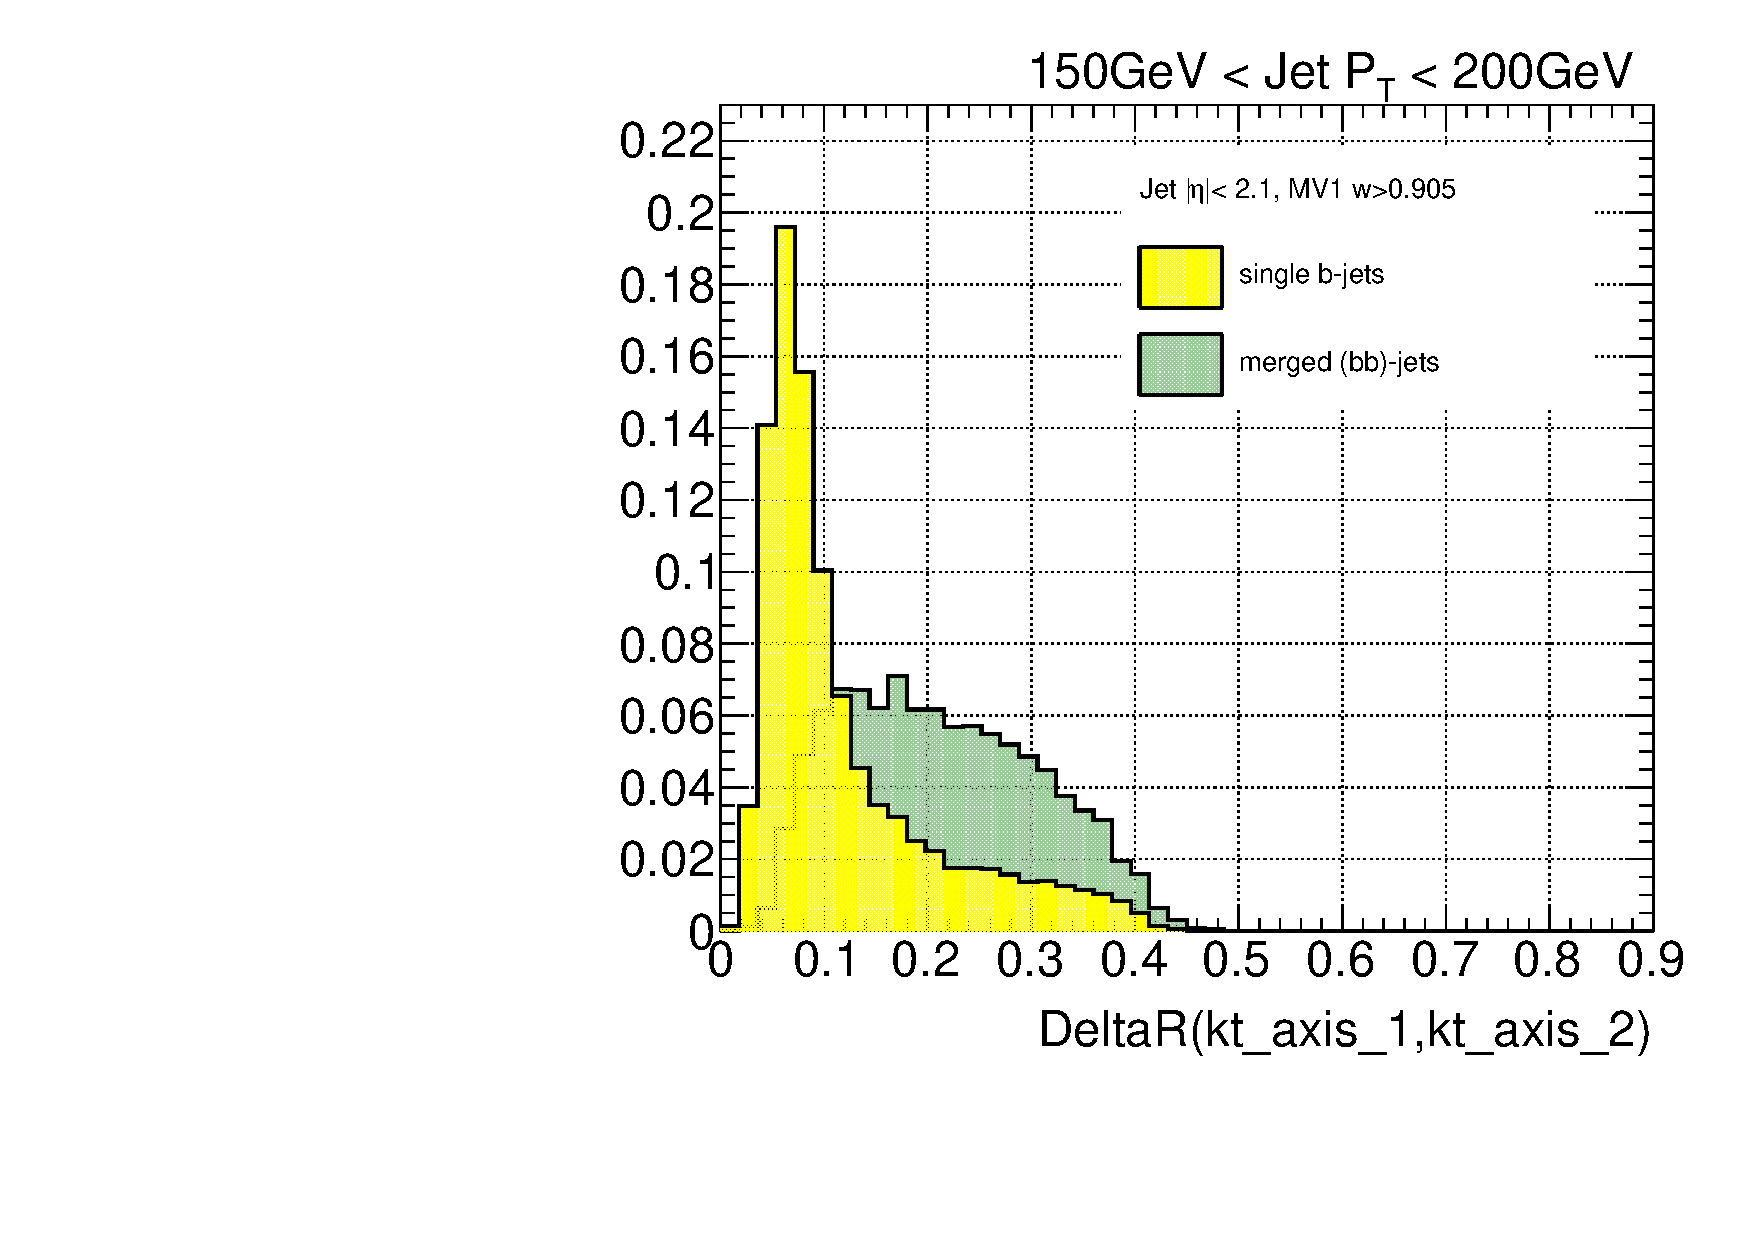
\includegraphics[width=0.49\textwidth]{FIGS/VarsSingleMerged/DRkt2axes150.pdf}
\caption{Distribution of the maximum $\Delta R$ between two $k_t$ axis in jets ($\Delta R_{\rm max}$) for single and merged $b$-jets between 60~GeV to 80~GeV (left) and 150~GeV to 200~GeV (right).}
\label{fig:drktsinglemerged}
\end{figure}

\begin{figure}[tp]
\centering
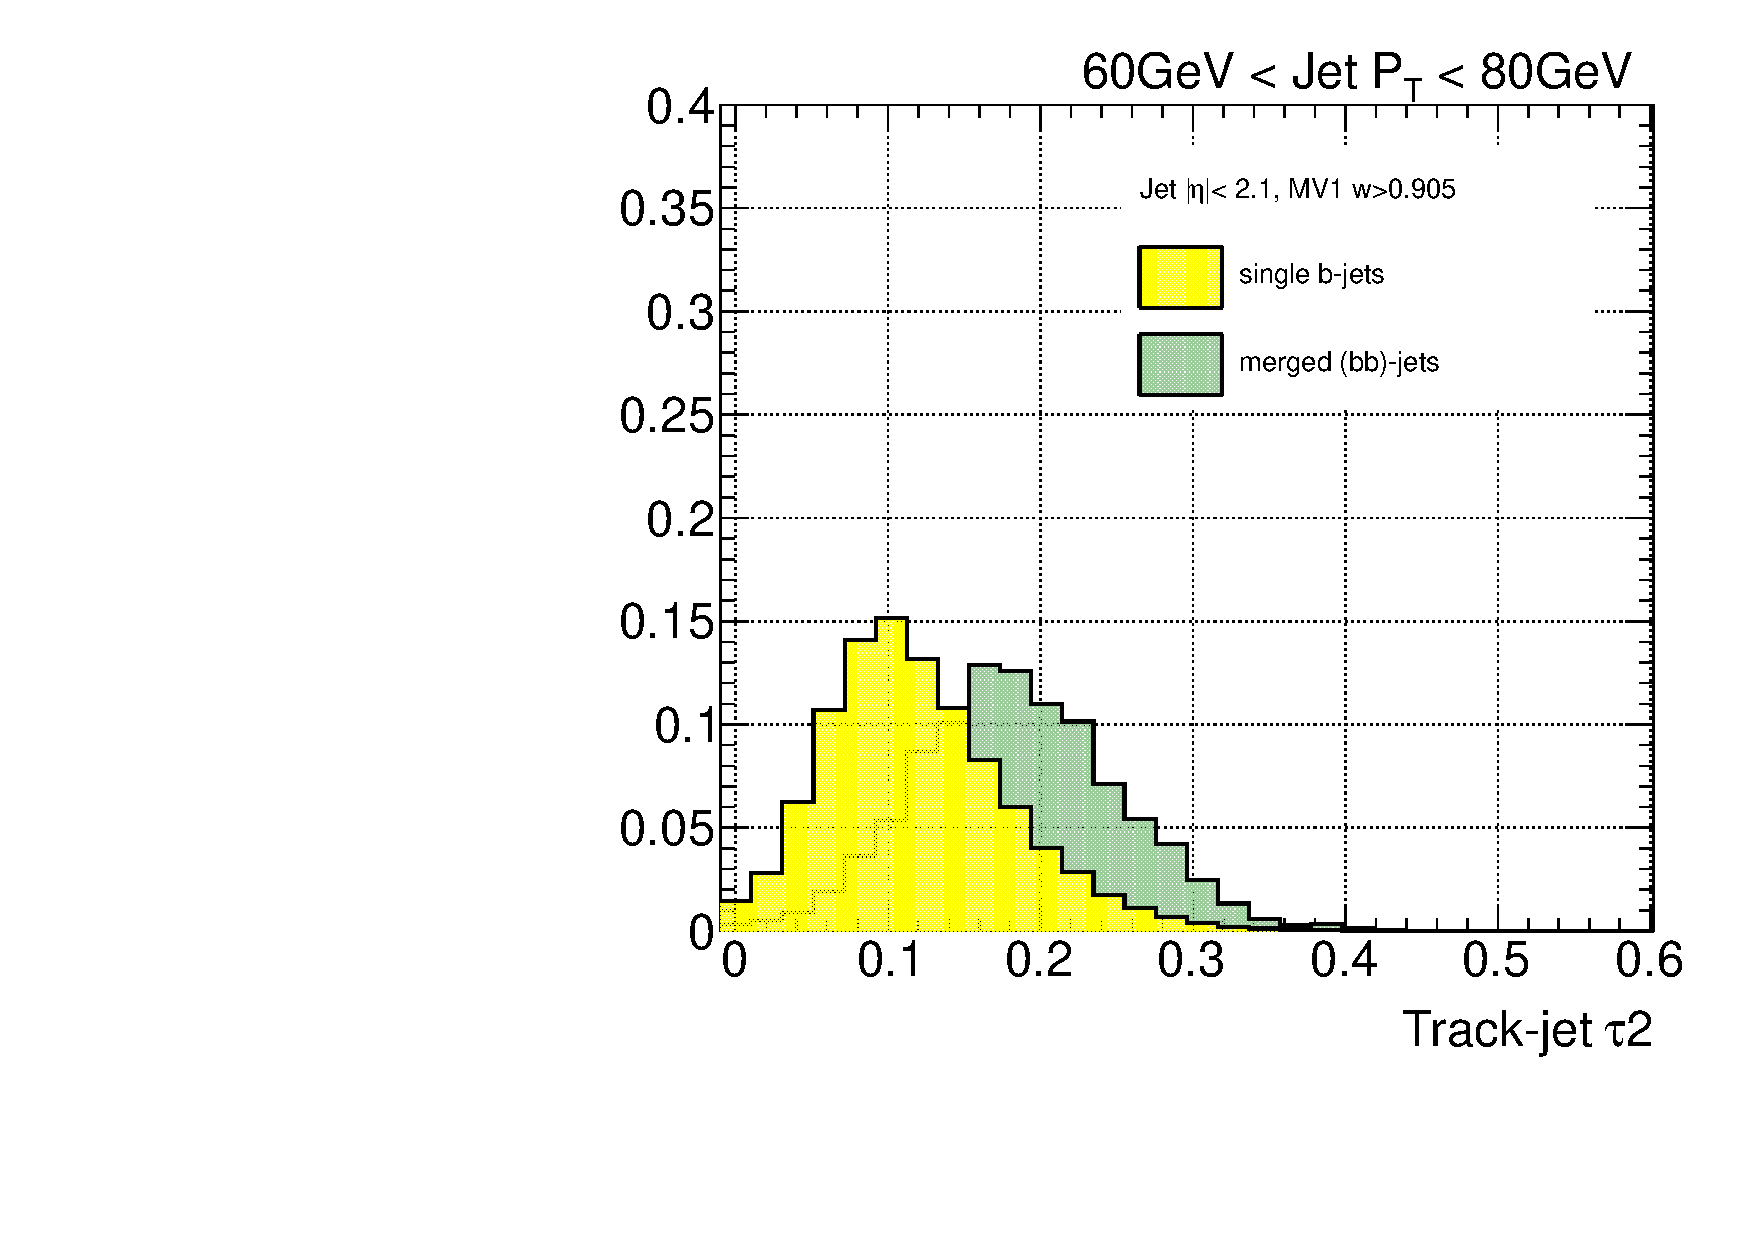
\includegraphics[width=0.49\textwidth]{FIGS/VarsSingleMerged/Tau2060.pdf}
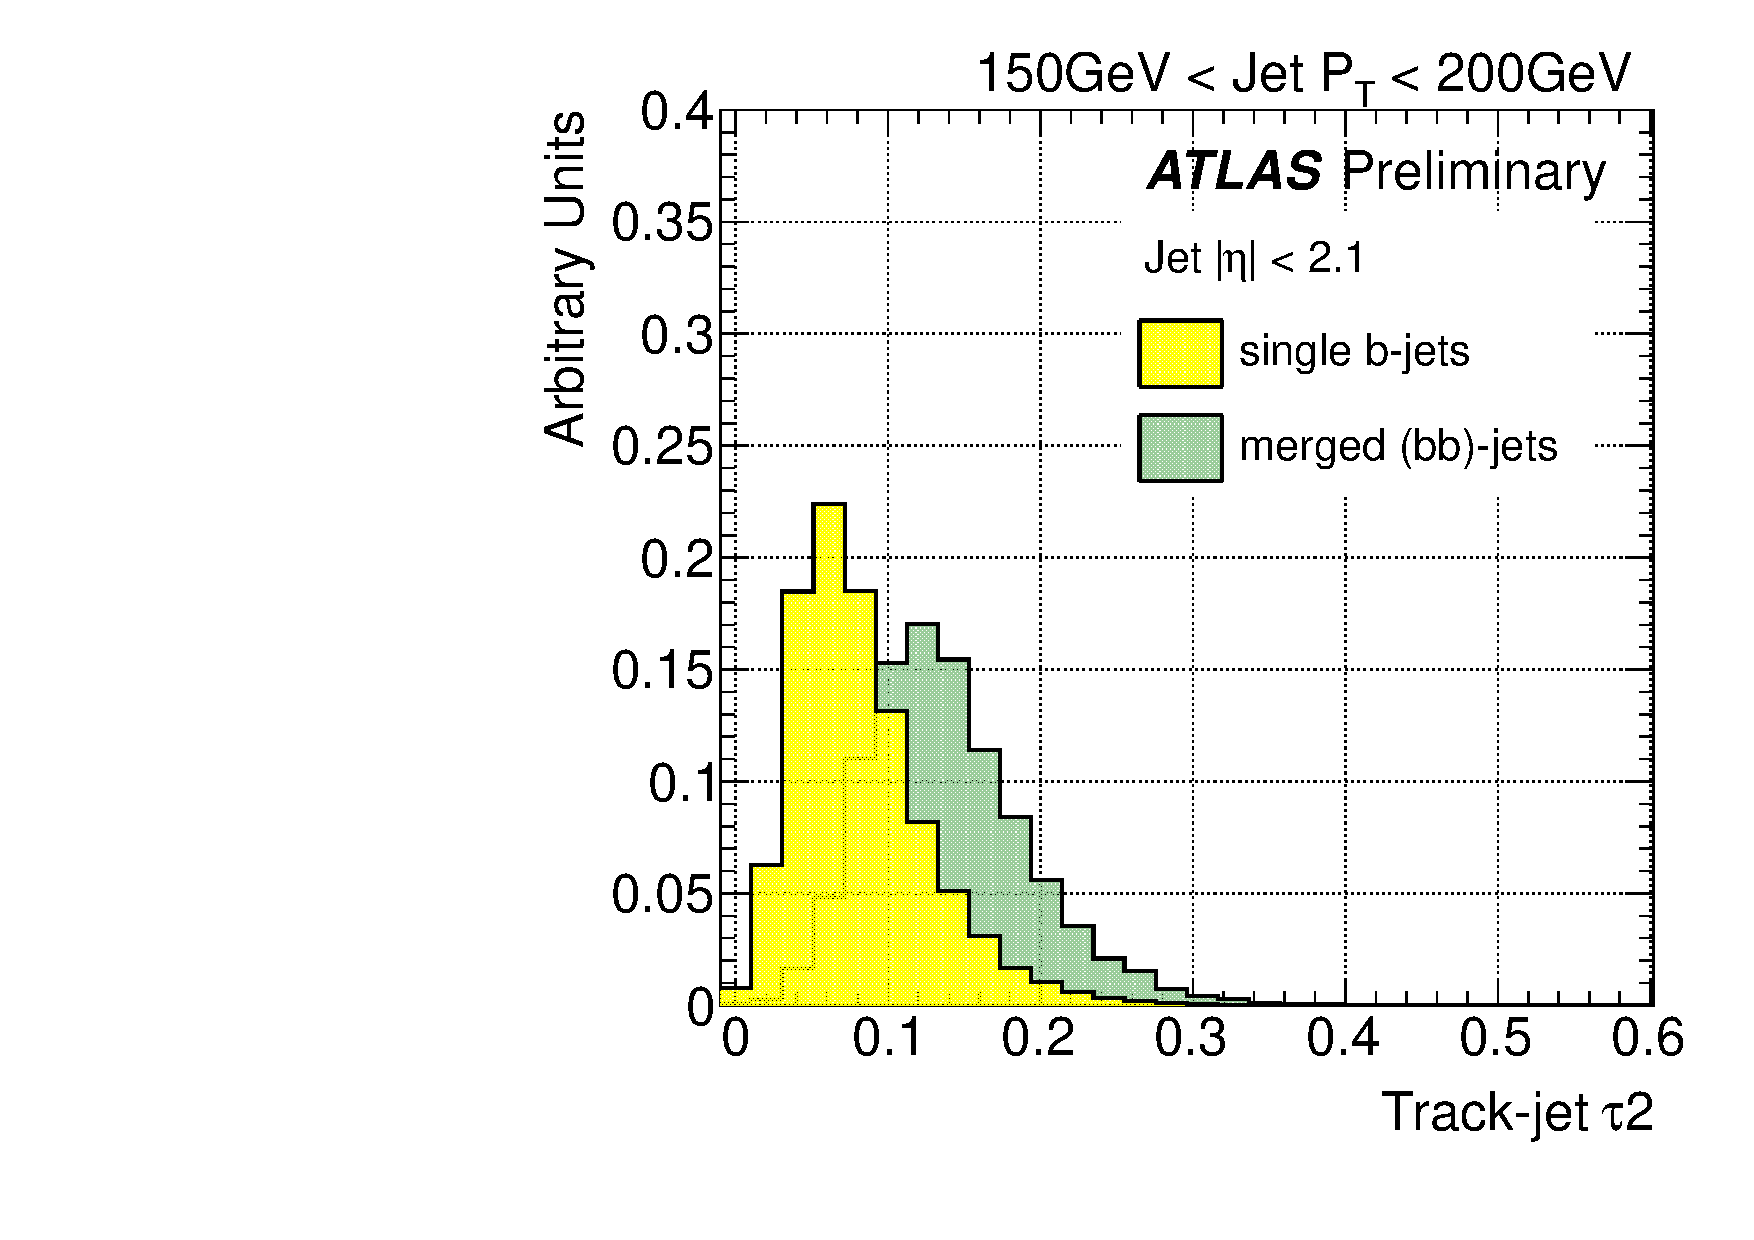
\includegraphics[width=0.49\textwidth]{FIGS/VarsSingleMerged/Tau2150.pdf}
\caption{Distribution of $\tau_2$ in jets for single and merged $b$-jets between 60~GeV to 80~GeV (left) and 150~GeV to 200~GeV (right).}
\label{fig:tau2singlemerged}
\end{figure}


\begin{figure}[tp]
\centering
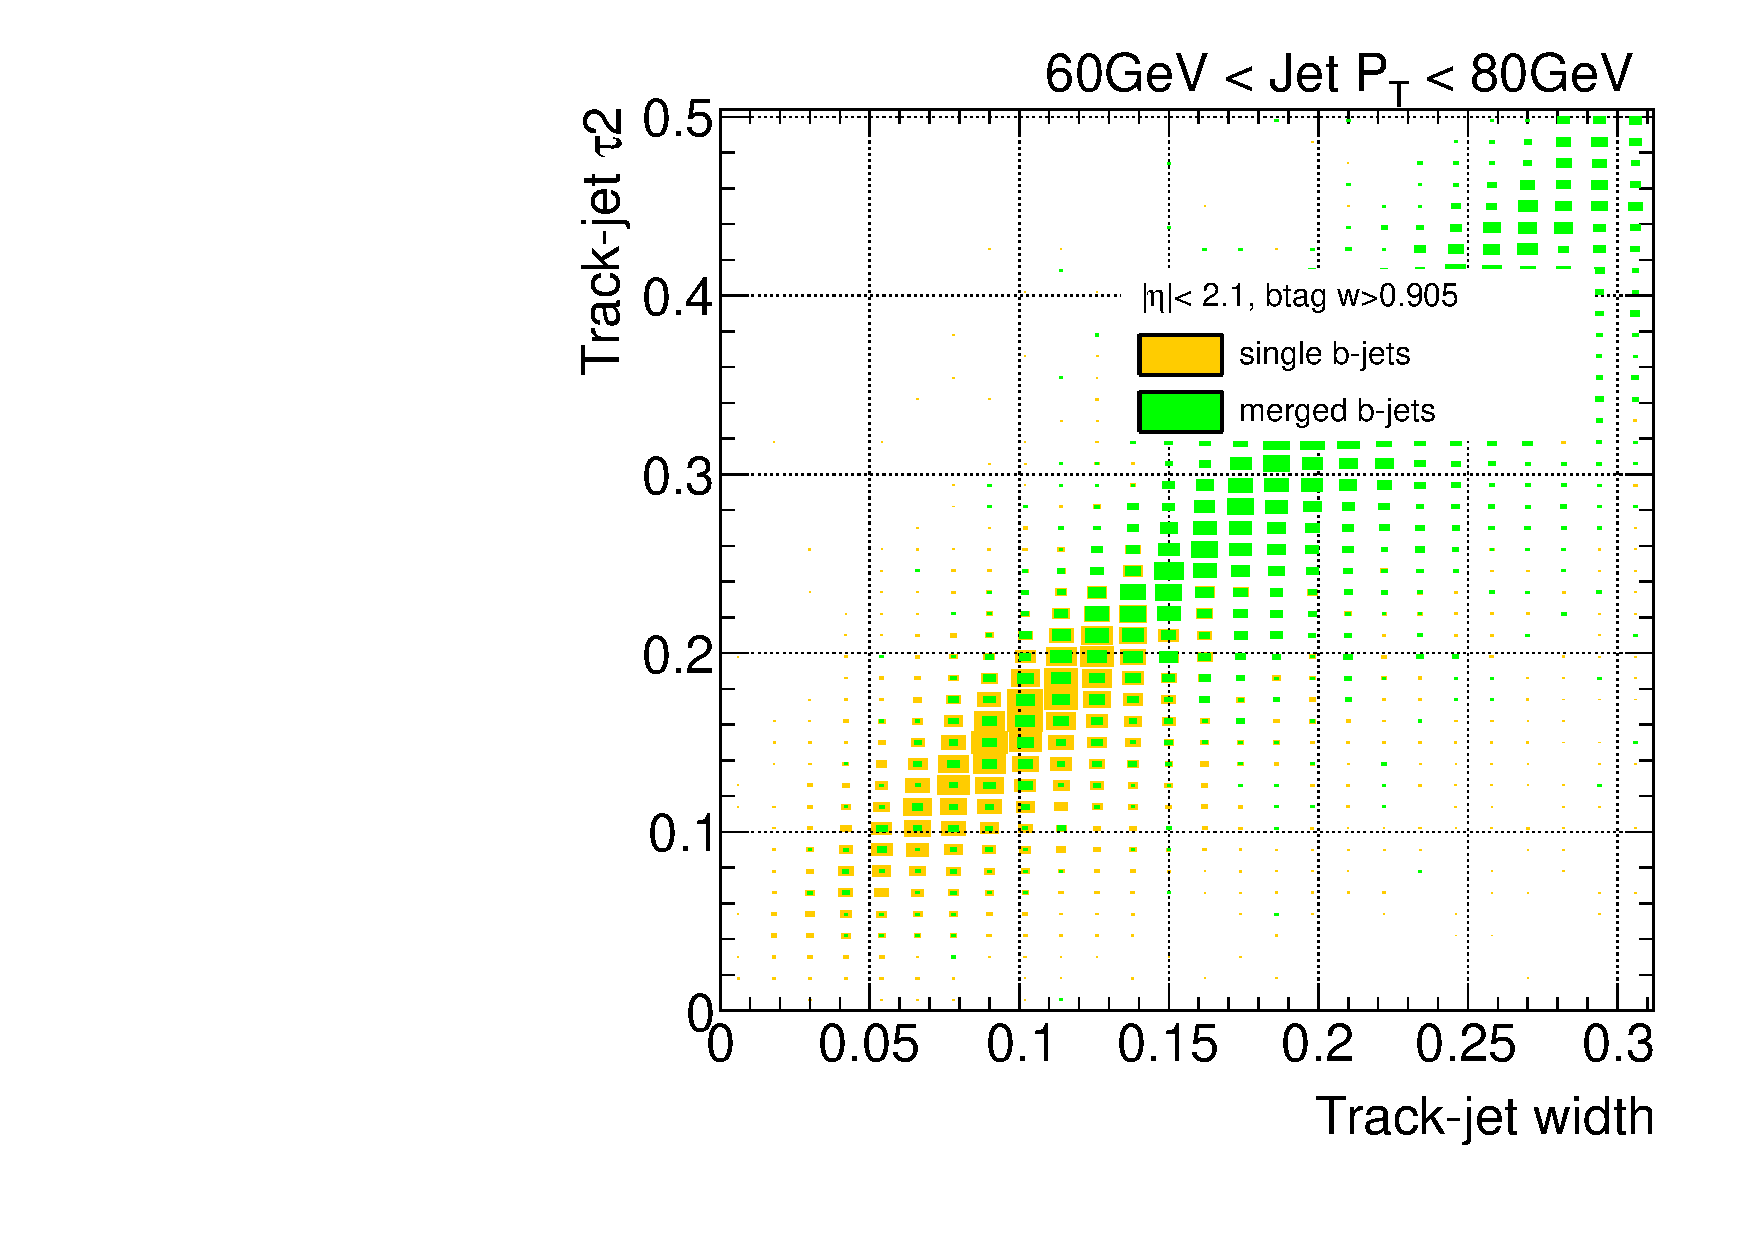
\includegraphics[width=0.49\textwidth]{FIGS/VarsSingleMerged/Tau2trkWidth060.pdf}
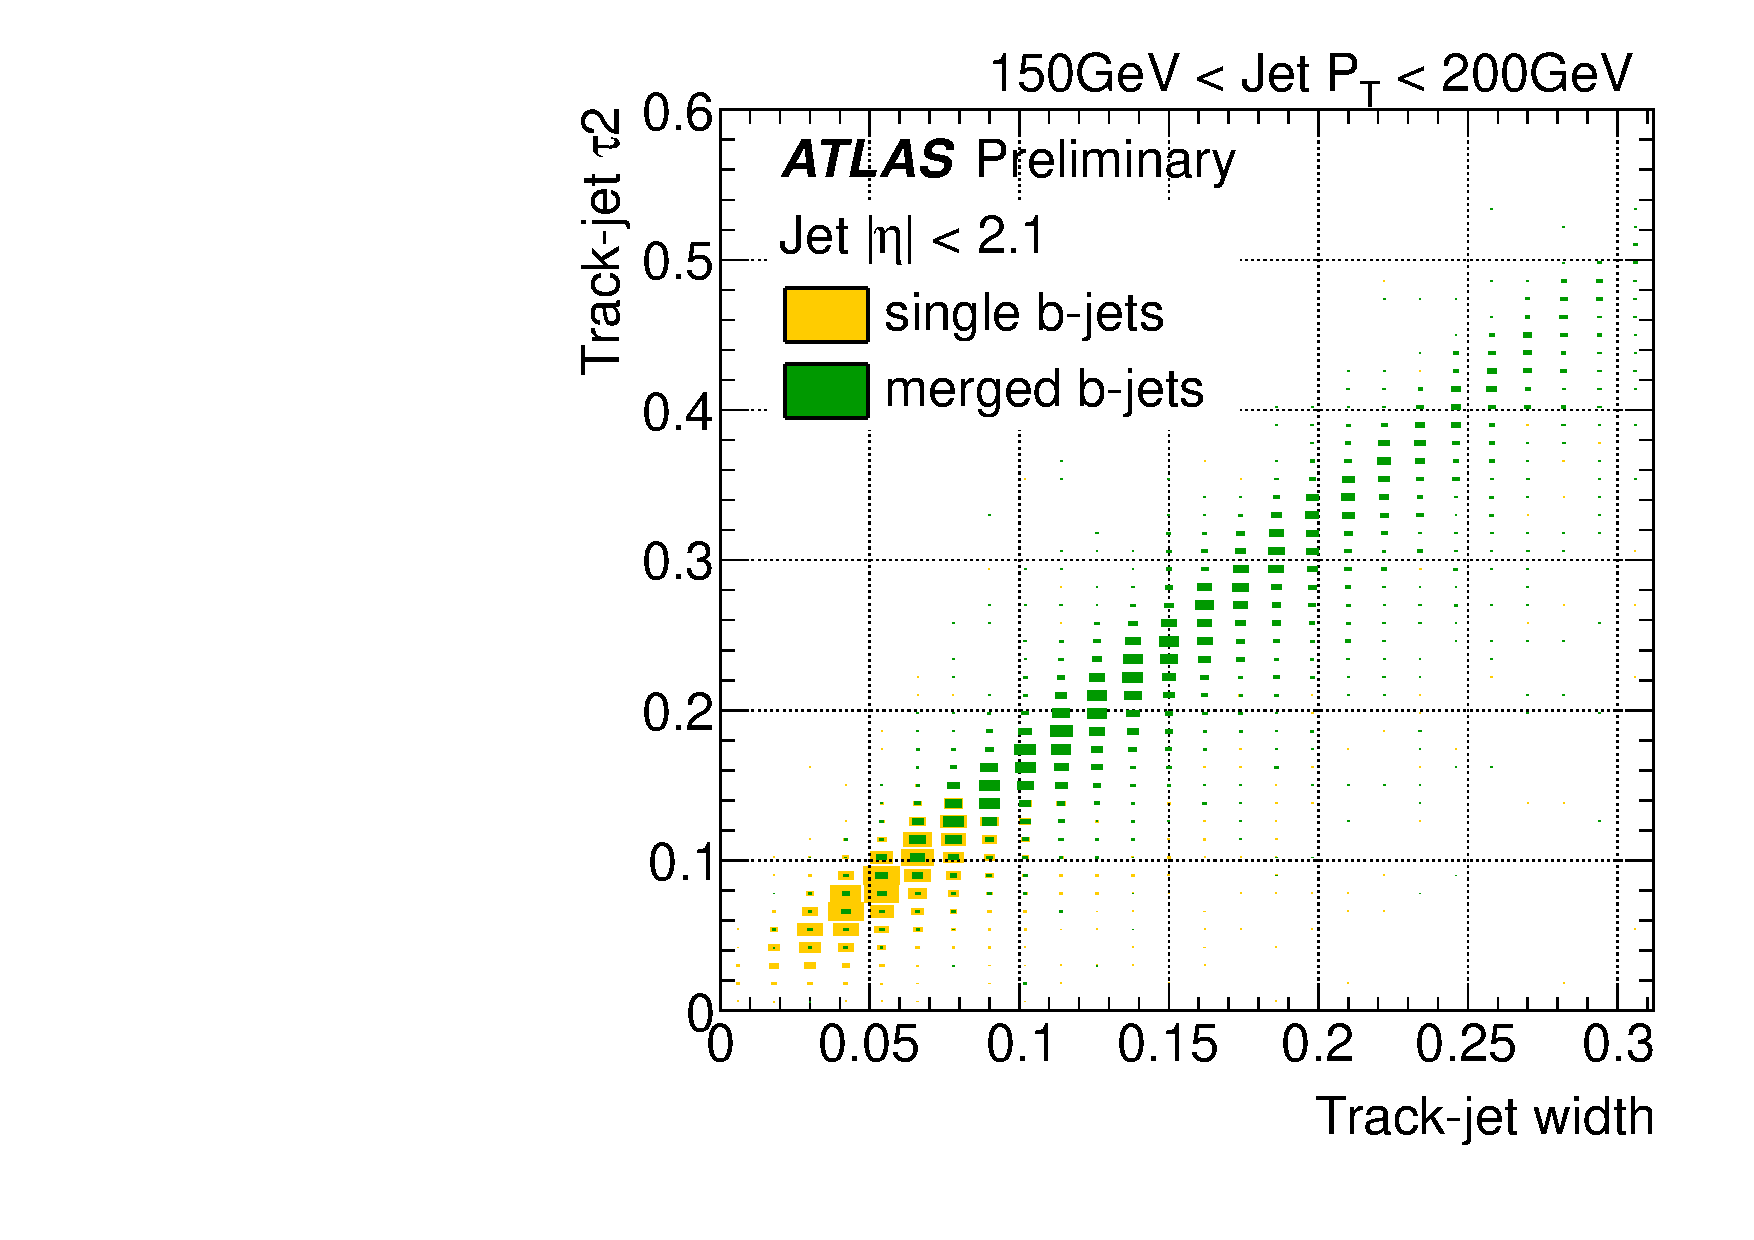
\includegraphics[width=0.49\textwidth]{FIGS/VarsSingleMerged/Tau2trkWidth150.pdf}
\caption{Correlation between $\tau _2$ and track-jet width for single and merged $b$-jets between 60~GeV to 80~GeV (left) and 150~GeV to 200~GeV (right).}
\label{fig:tau2trkwidthsinglemerged}
\end{figure}

\begin{figure}[tp]
\centering
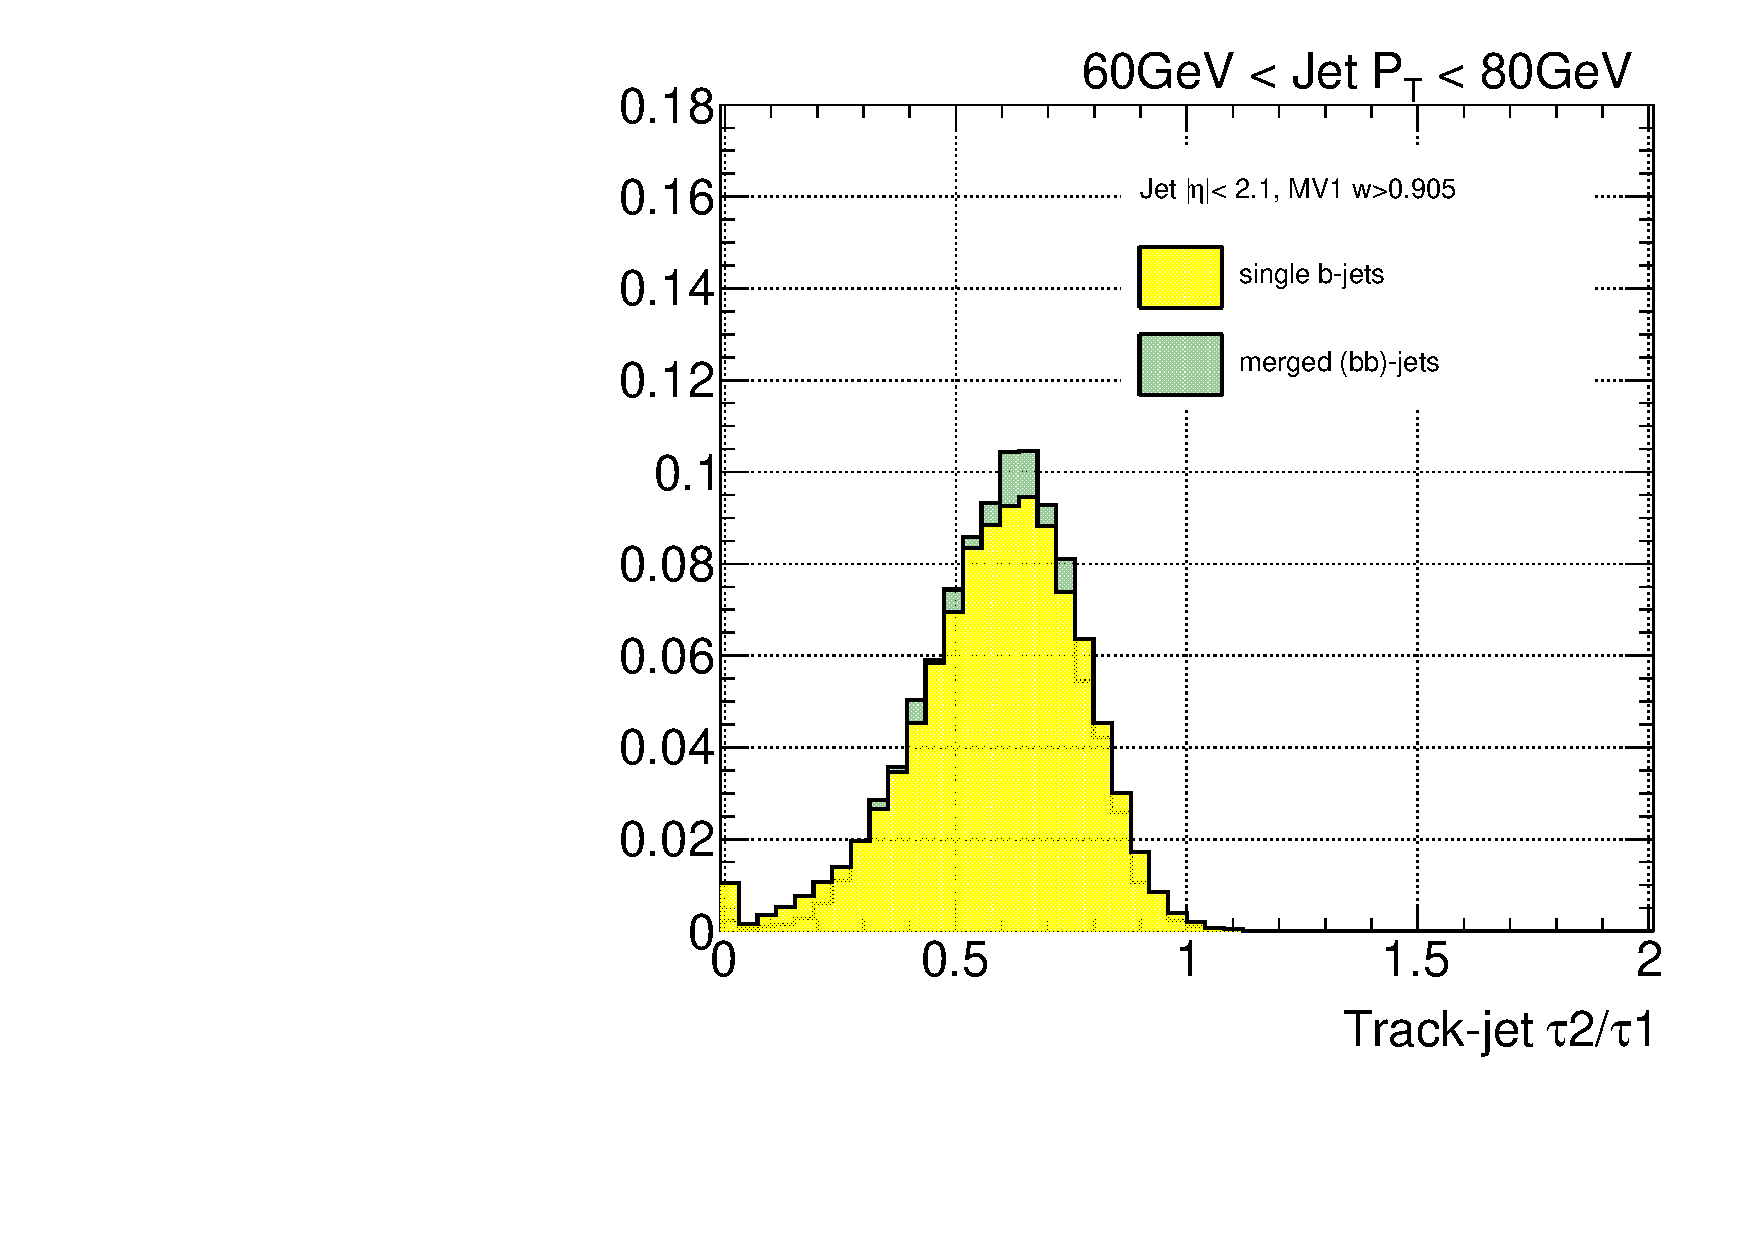
\includegraphics[width=0.49\textwidth]{FIGS/VarsSingleMerged/TauRatio060.pdf}
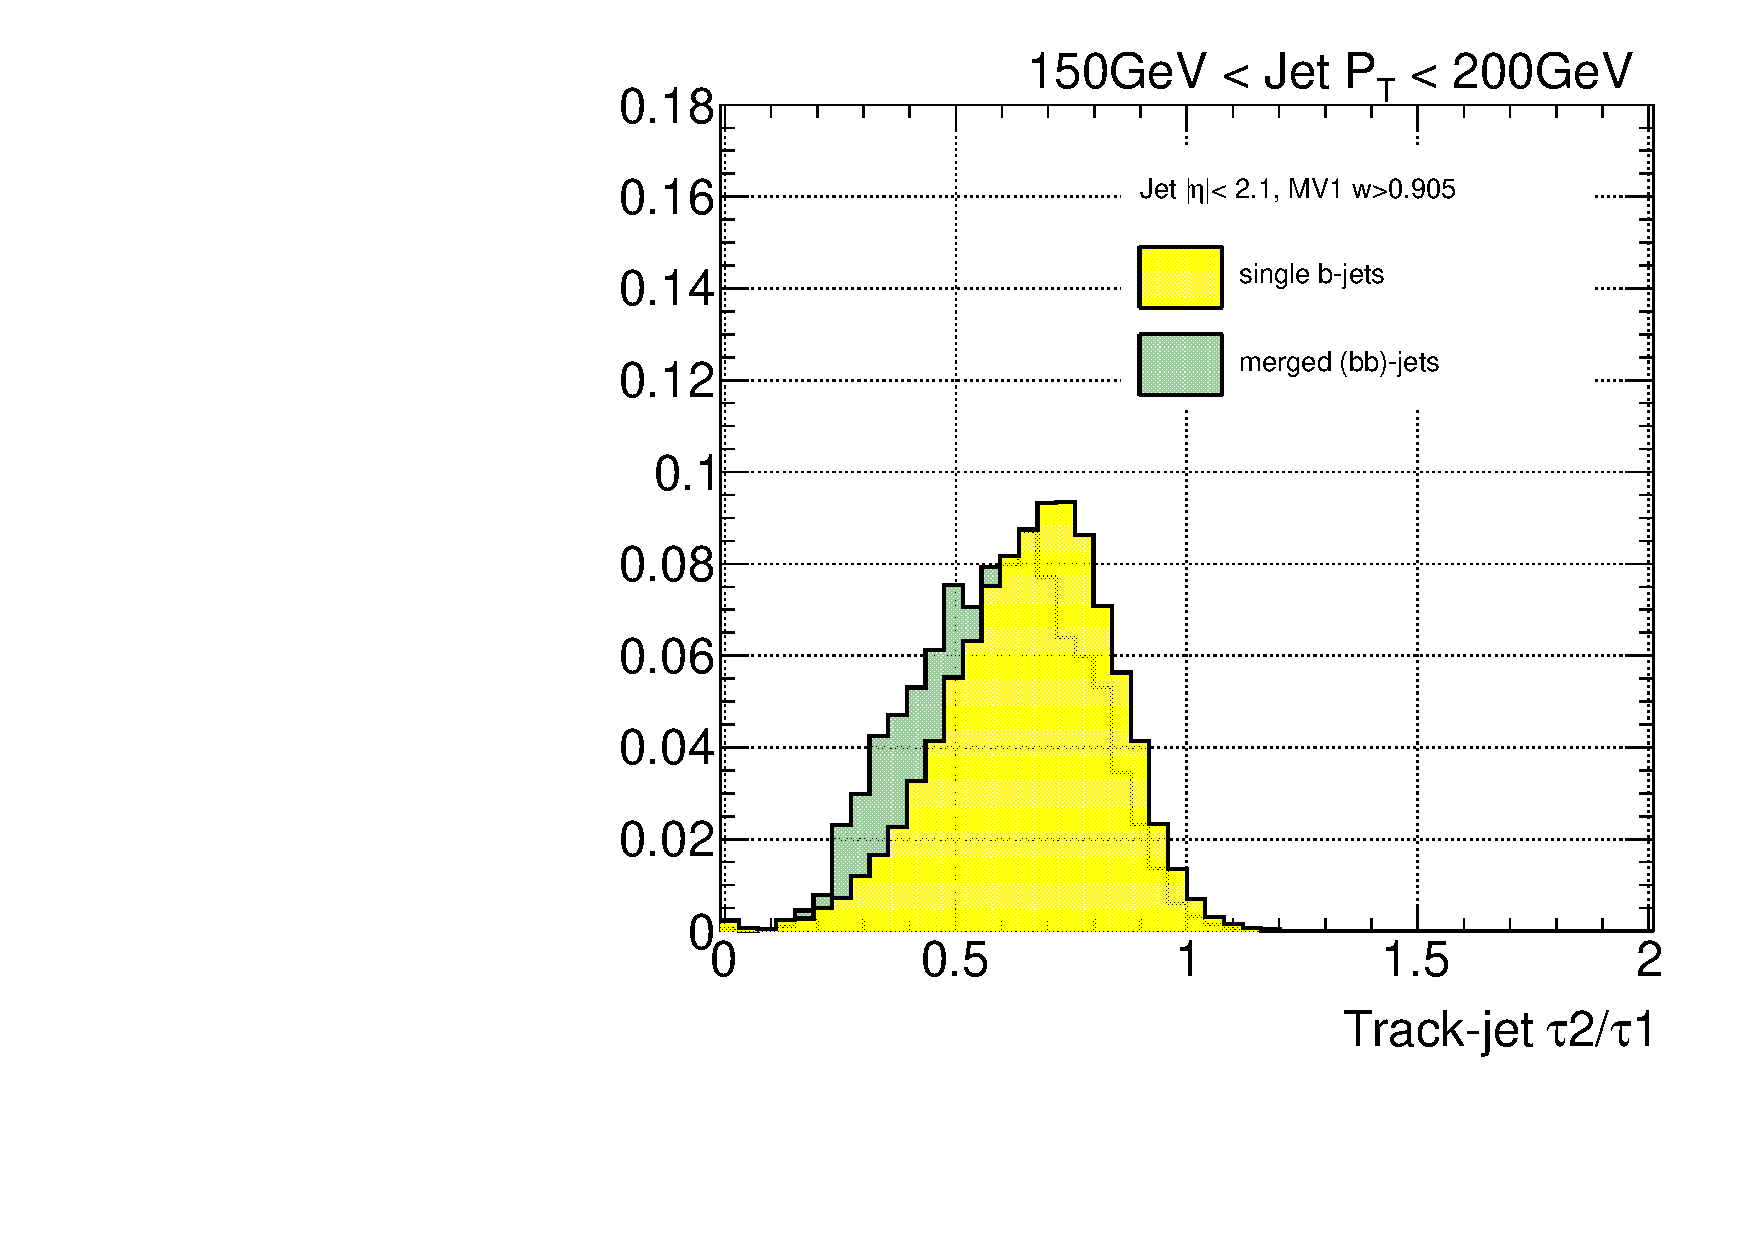
\includegraphics[width=0.49\textwidth]{FIGS/VarsSingleMerged/TauRatio150.pdf}
\caption{Distribution of $\tau_2/\tau_1$ in jets for single and merged $b$-jets between 60~GeV to 80~GeV (left) and 150~GeV to 200~GeV (right).}
\label{fig:tauratiosinglemerged}
\end{figure}


%We also explored the potential improvement of constructing kinematic variables with only displaced tracks, as these are the ones expected to arise from the decay of B-hadrons. Cuts of 2, 2.5 and 3 on the track transverse impact parameter significance were investigated leading however to no gain in discrimation power.  


%------------------------------------------------------------------------
\section{Validation of the jet variables in data}\label{sec:gbbValidation}
%------------------------------------------------------------------------
In order to study the extent to which the simulation reproduces the distributions observed in data for the different variables explored a set comparison plots is presented. Fig.~\ref{fig:datamcinputvars} shows the distributions of $N_{\it trk}$, track-jet width ($\pt$ weighted) and $\Delta {\rm R}_{k_{\rm T}}$ in two different jet $\pt$ bins in dijet Monte Carlo and data events from periods B to H overlaid. The distributions are normalized to unit area to allow for shape comparisons. There is a good agreement between data and simulation. 

 For the sake of evaluating the effect of the increasing amount of pile-up in the last periods of data-taking, %affected the agreement between experimental data and Monte Carlo
the same distributions were built using data events from periods I to M. As expected, no variation was observed. In Fig.~\ref{fig:datamcinputvarsItoM} the track-multiplicity is shown for these periods, in the same two $\pt$ bins for comparison.  

\begin{figure}[tp]
\centering
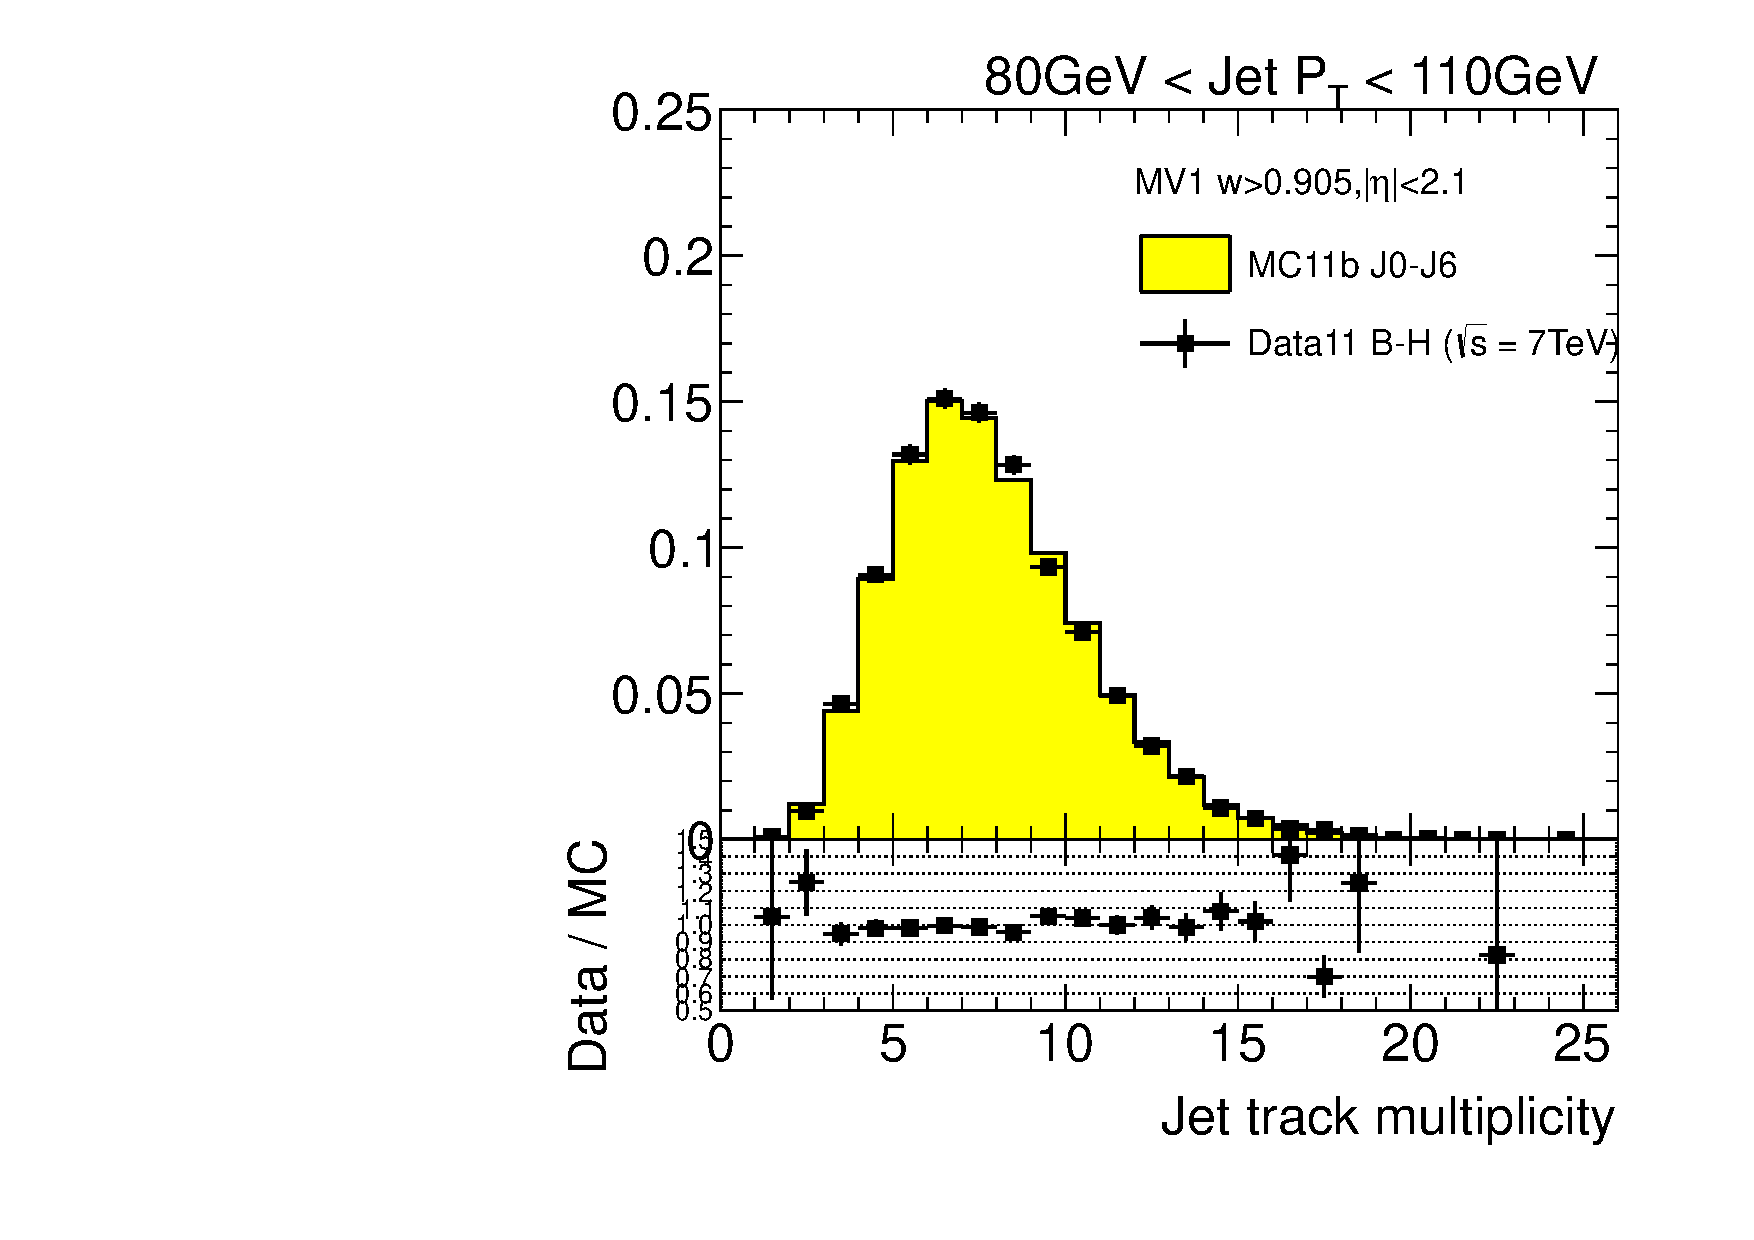
\includegraphics[width=0.49\textwidth]{FIGS/dataMC/VarNtrkPT080.pdf}
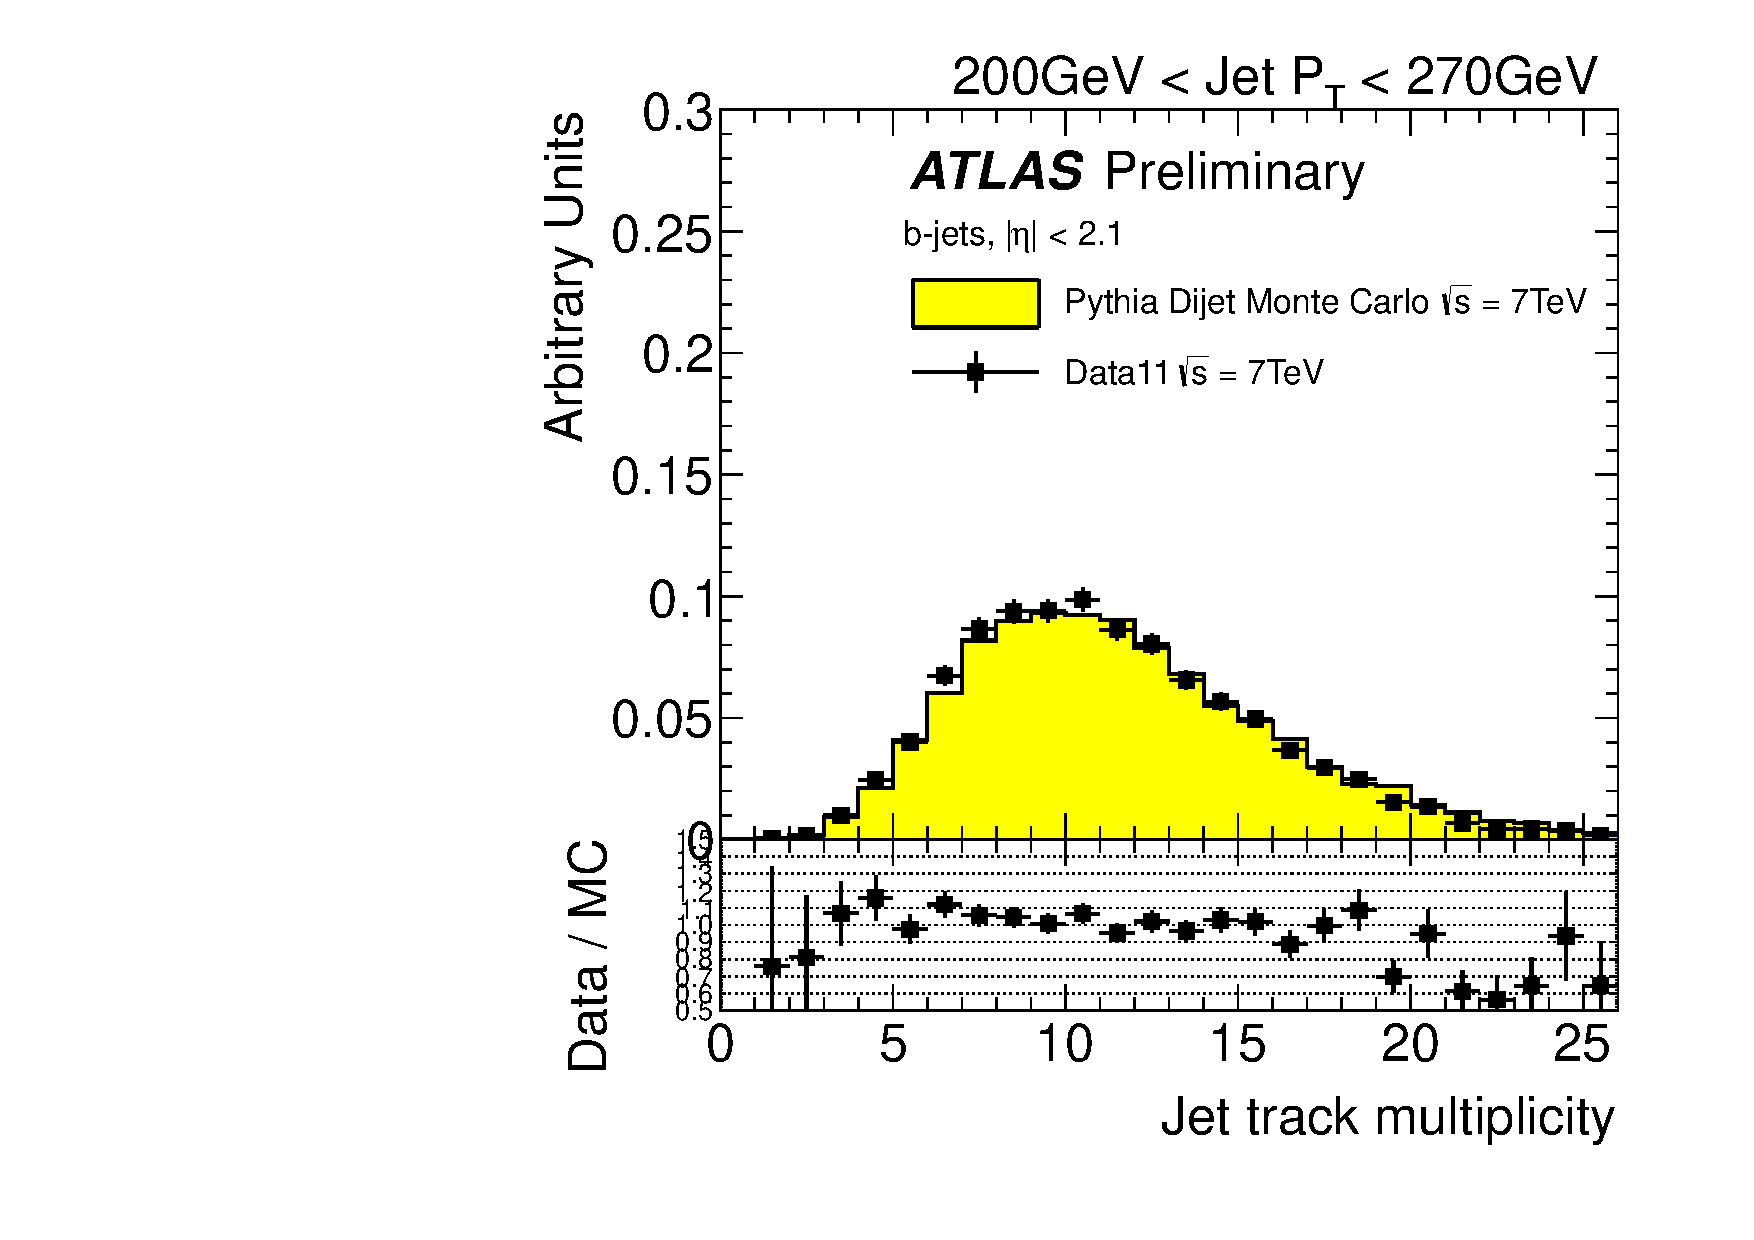
\includegraphics[width=0.49\textwidth]{FIGS/dataMC/VarNtrkPT200.pdf}
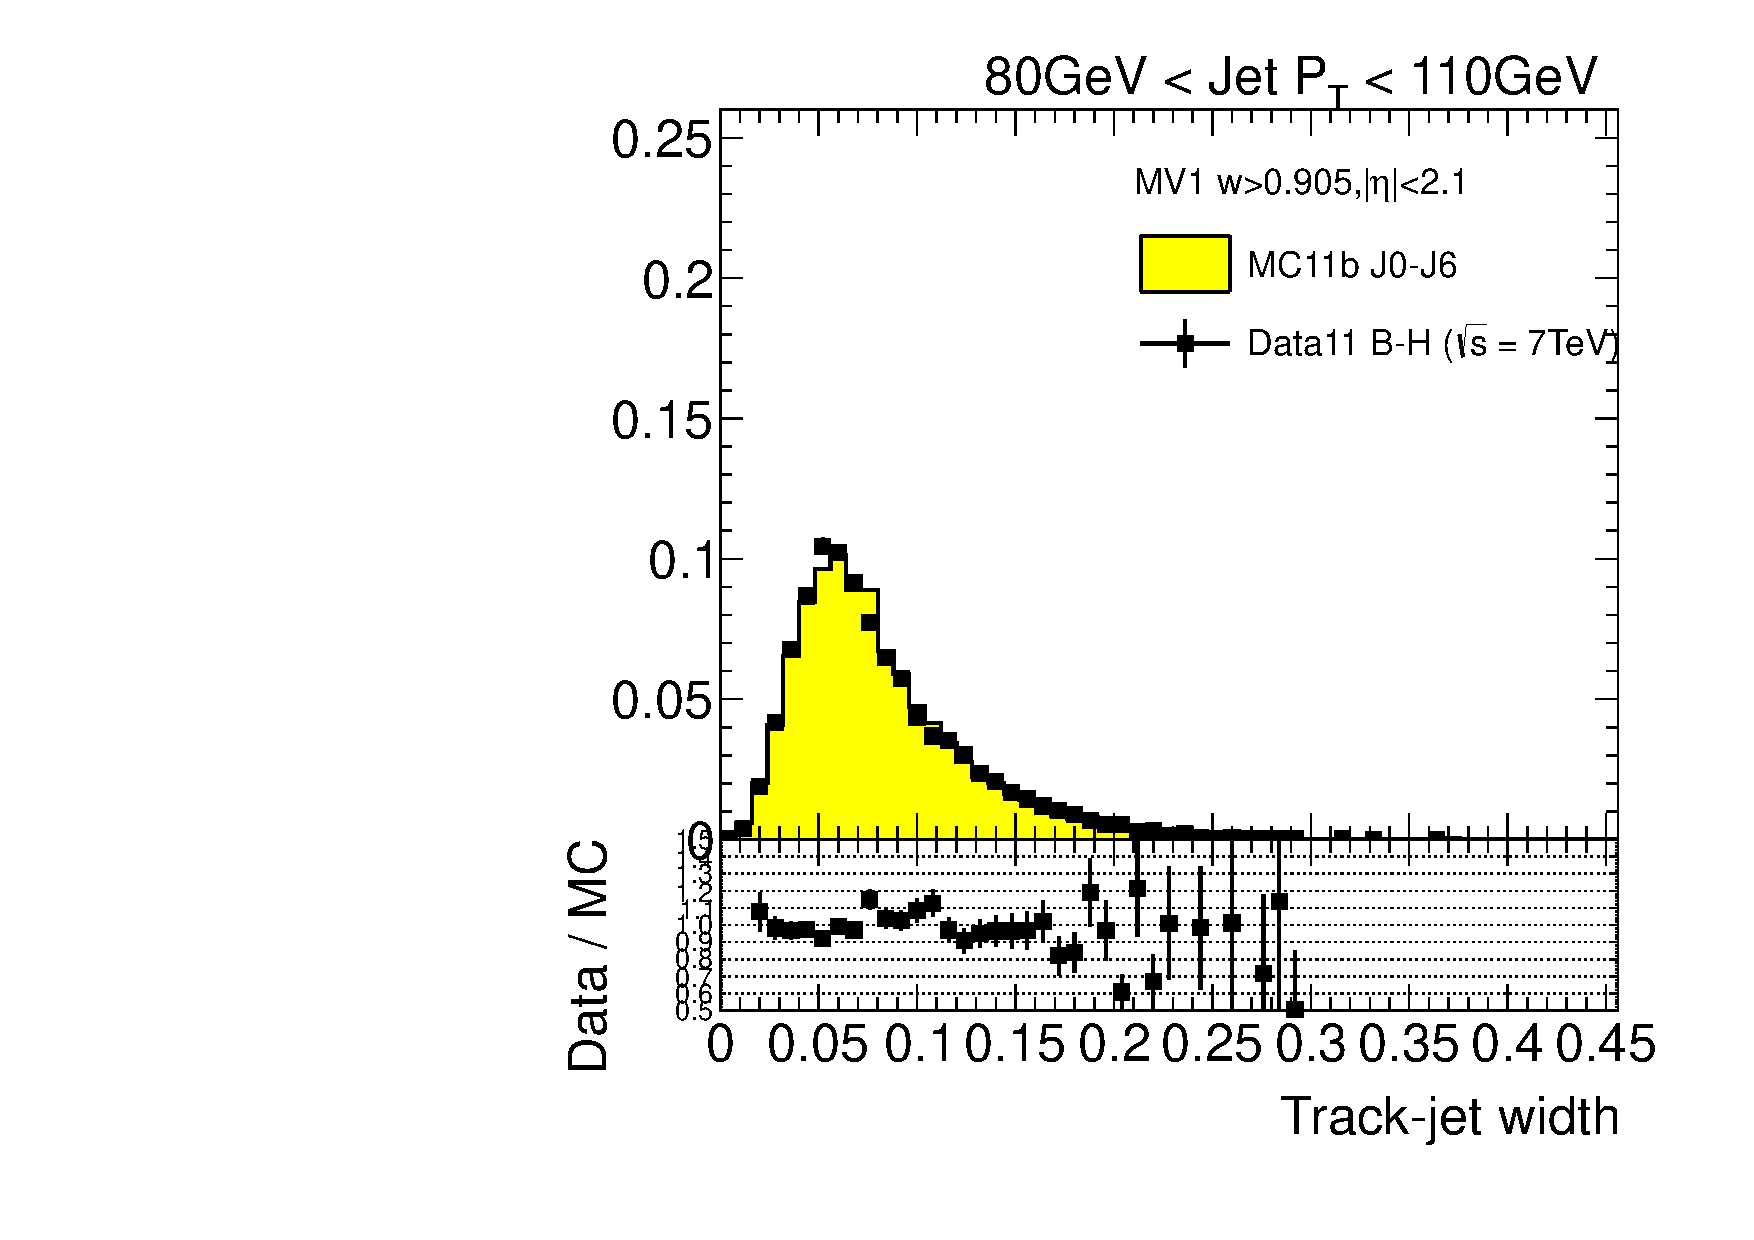
\includegraphics[width=0.49\textwidth]{FIGS/dataMC/VarTrkWidthPT080.pdf}
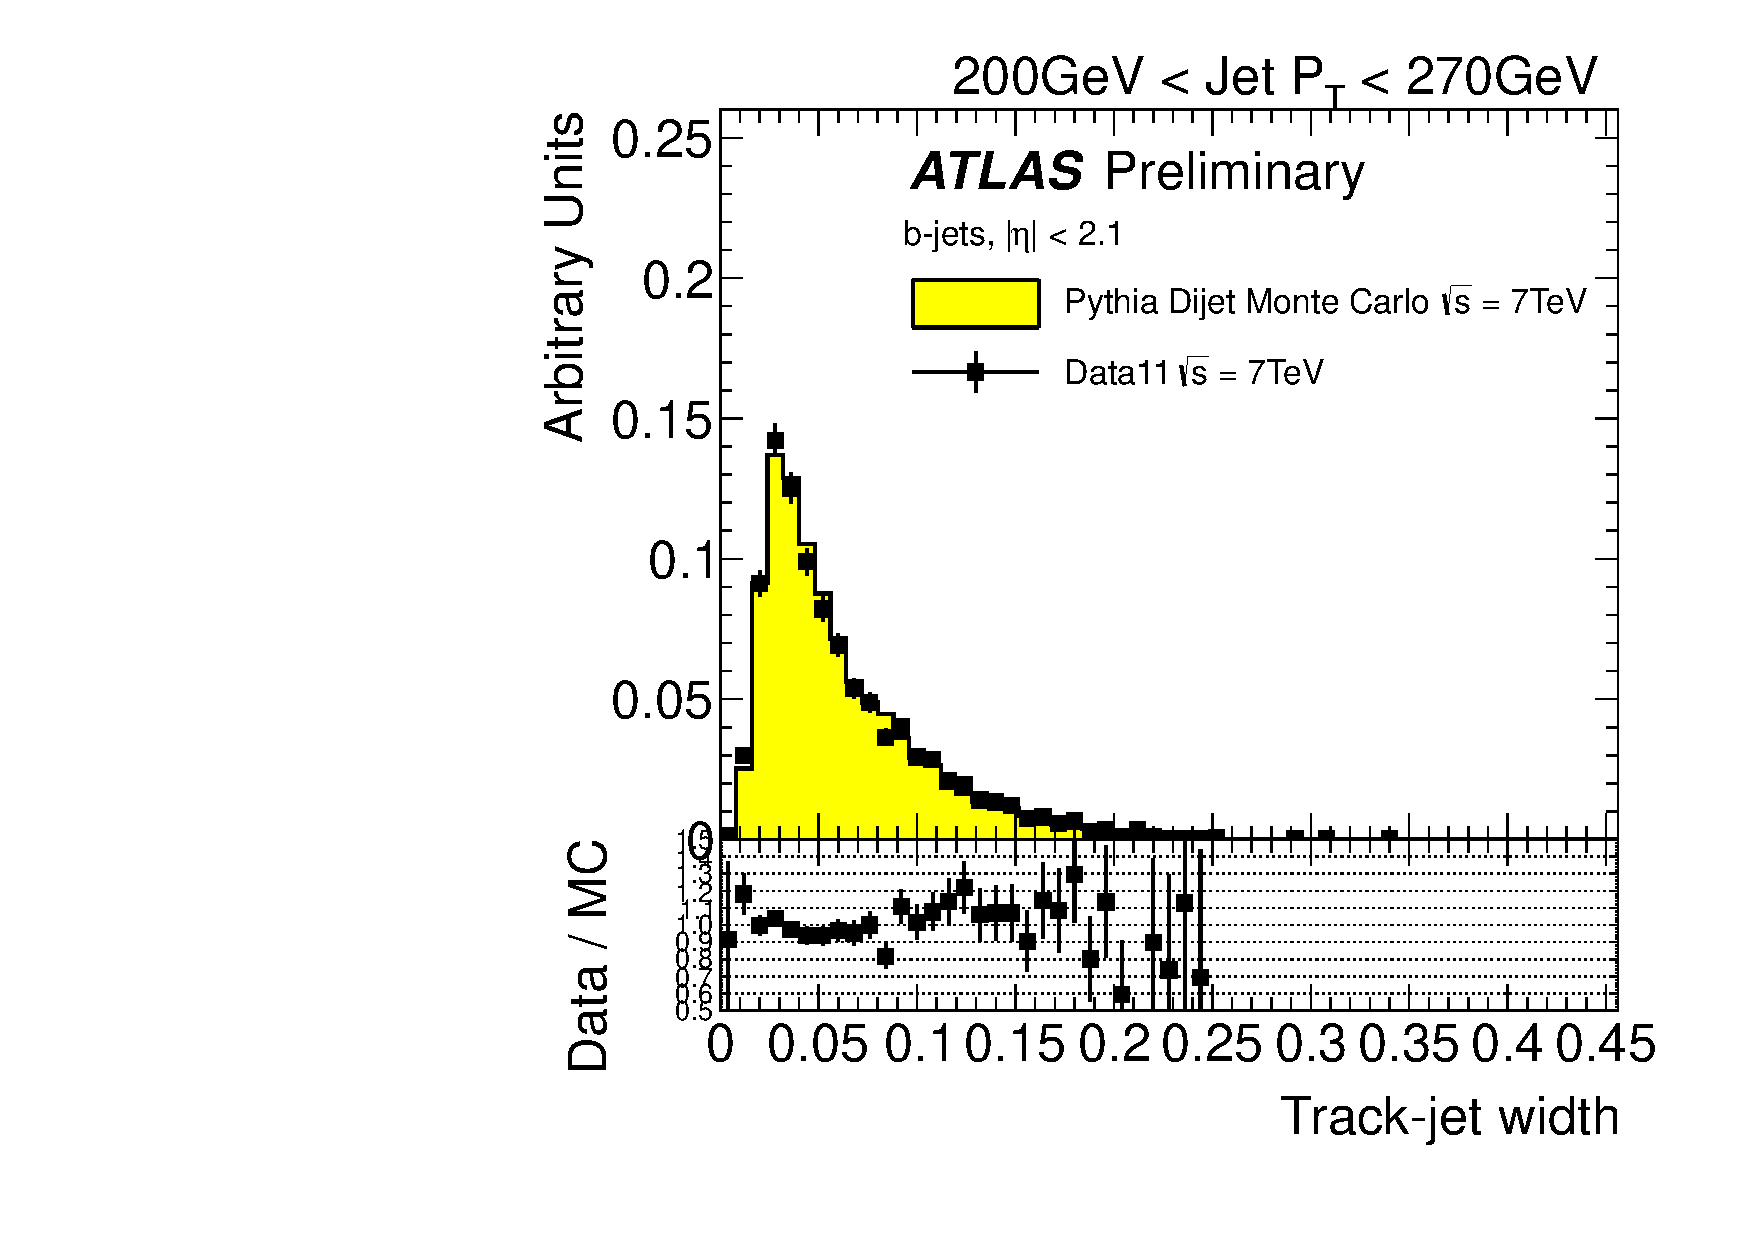
\includegraphics[width=0.49\textwidth]{FIGS/dataMC/VarTrkWidthPT200.pdf}  
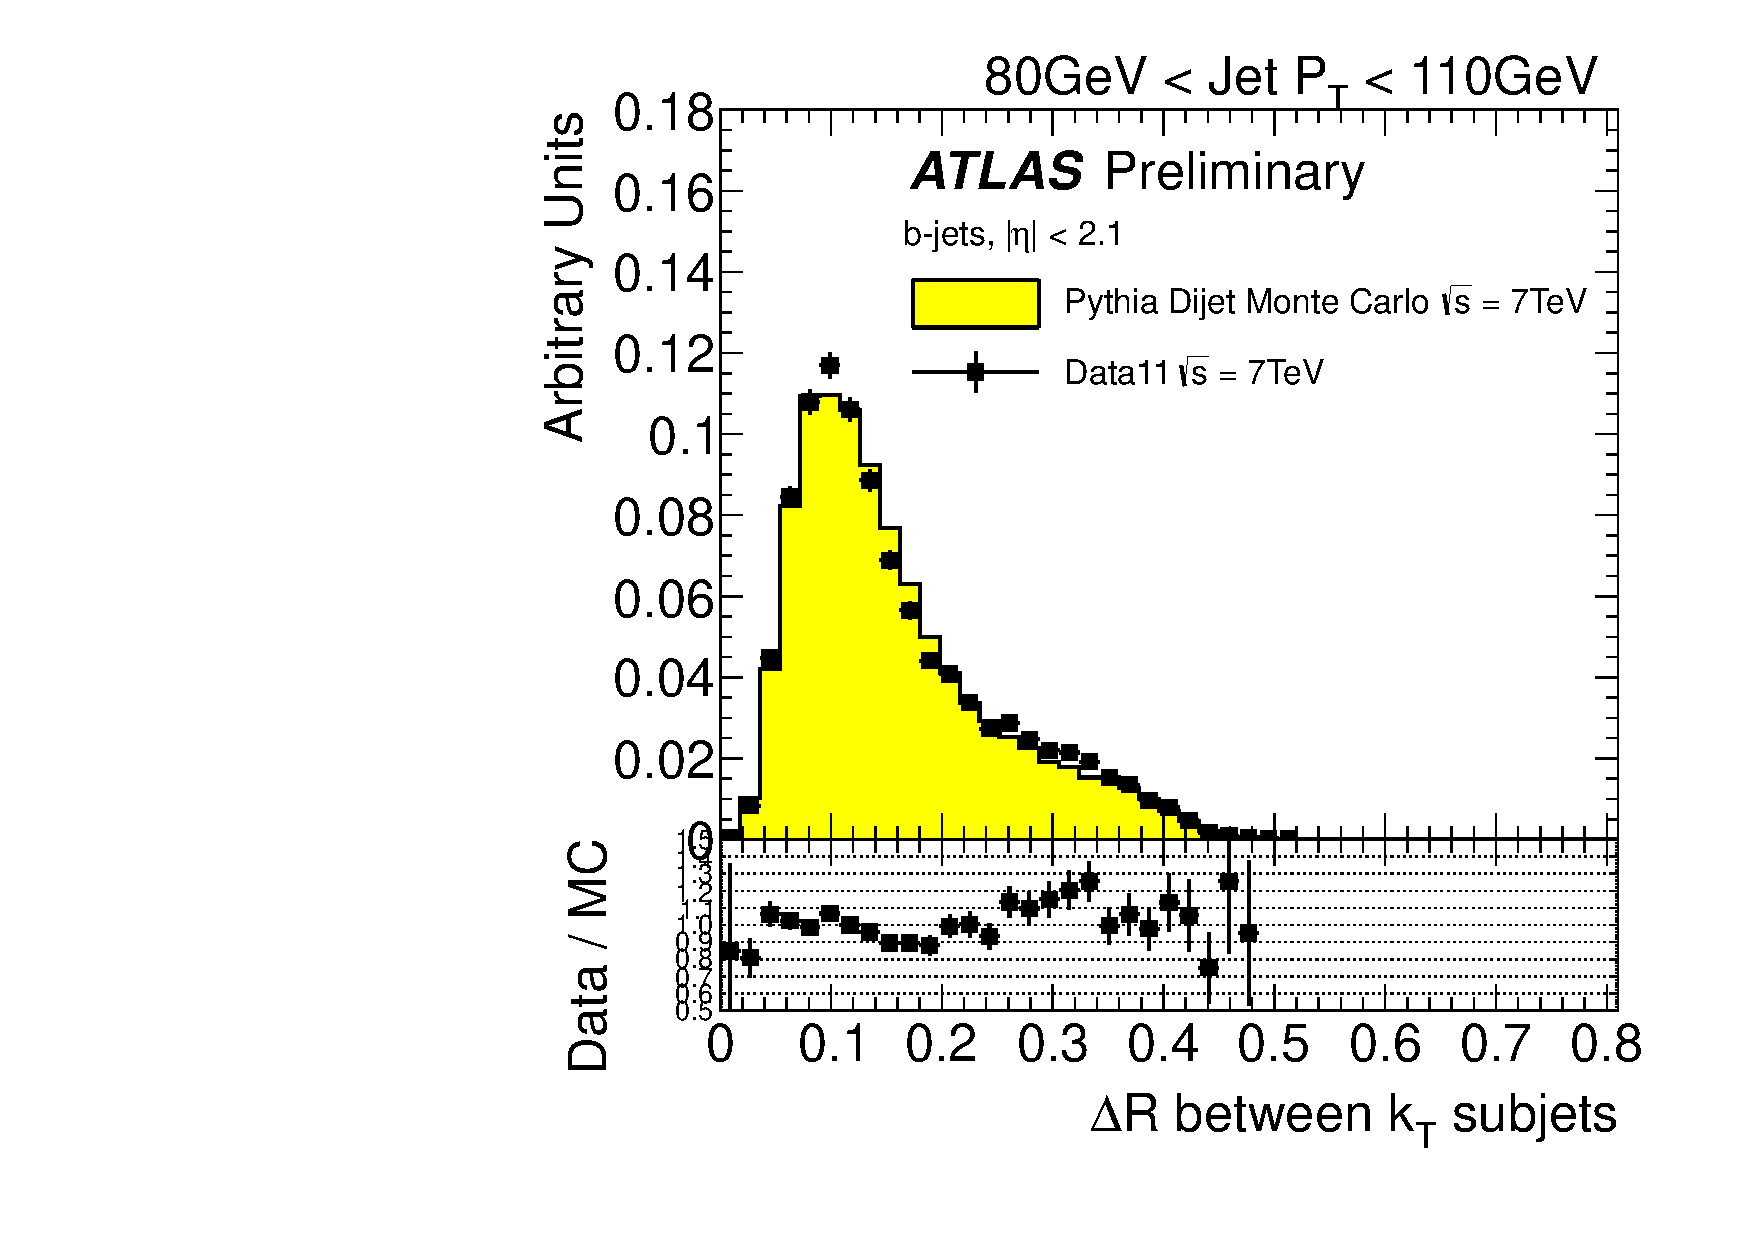
\includegraphics[width=0.49\textwidth]{FIGS/dataMC/VarDRktaxisPT080.pdf}
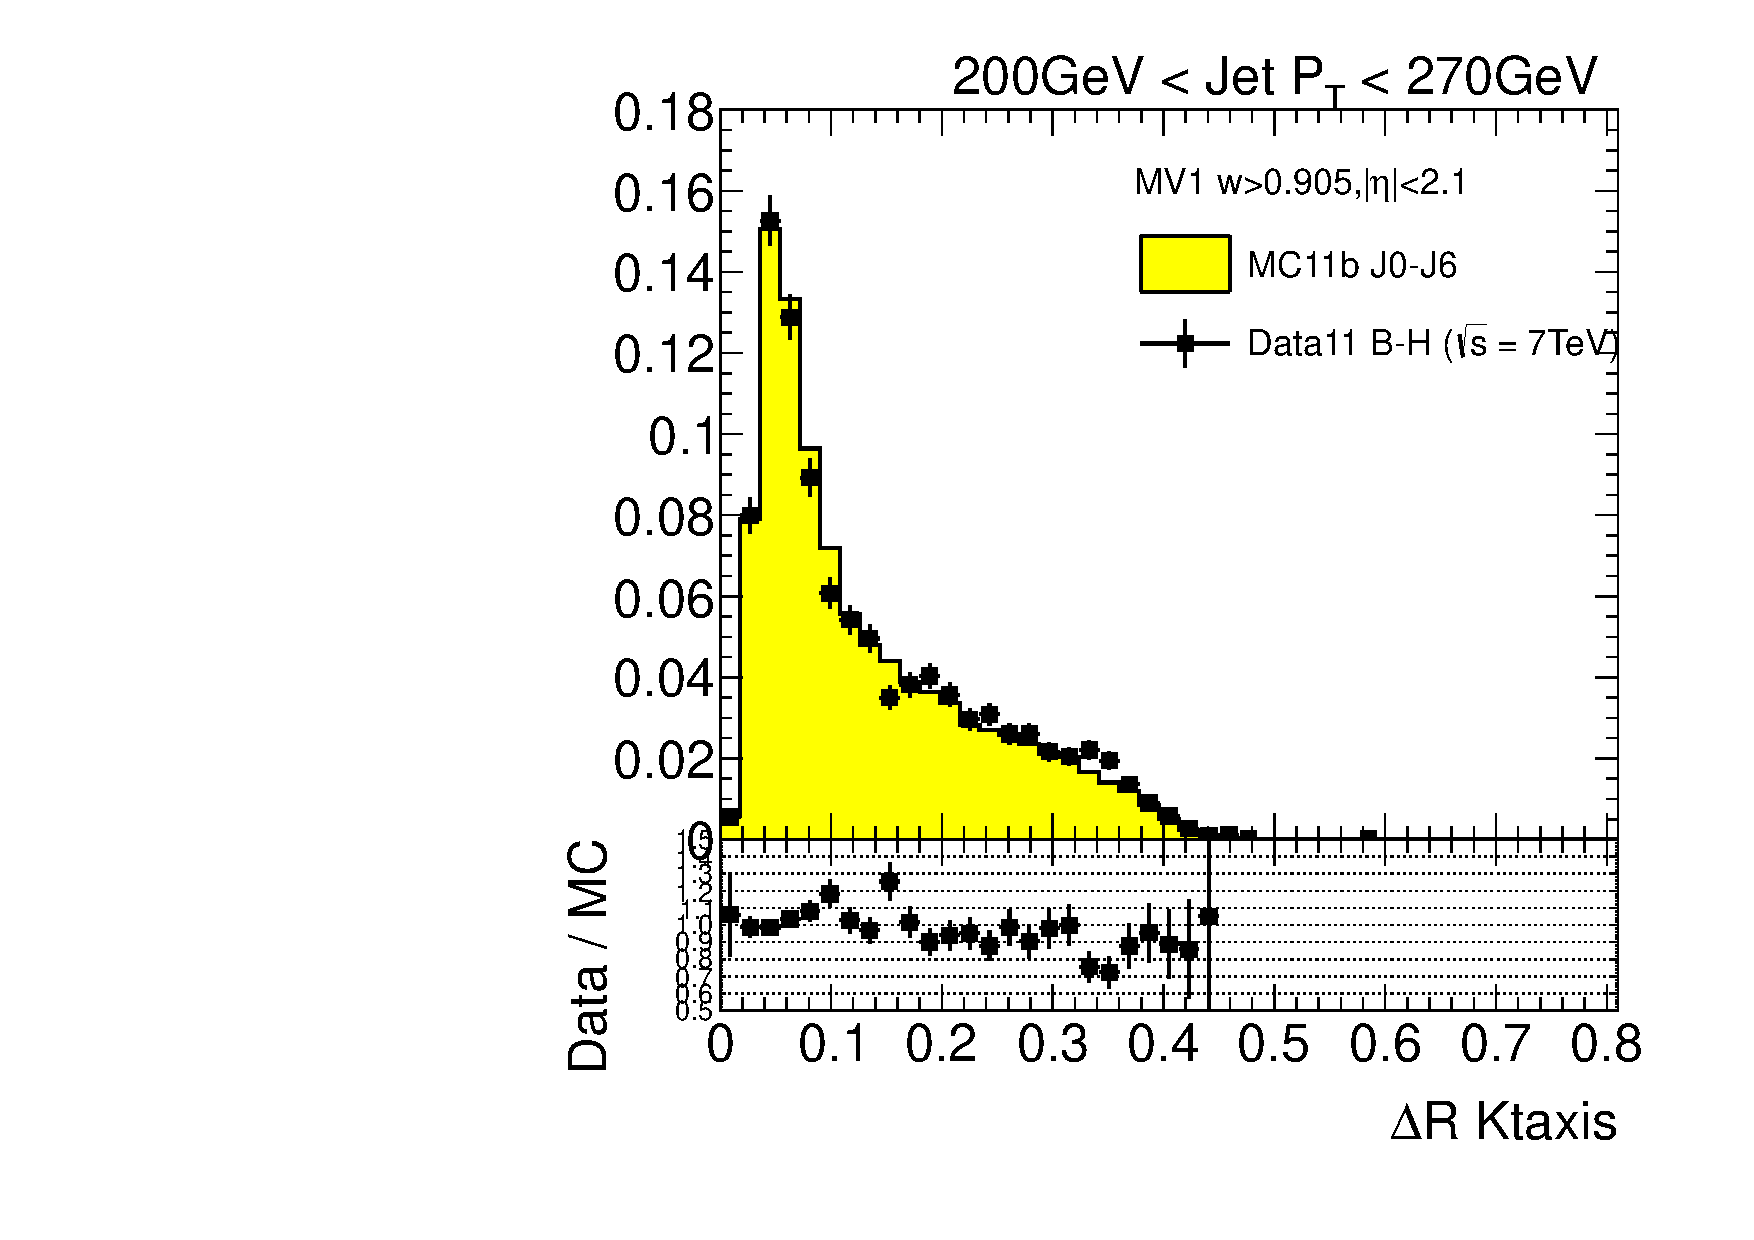
\includegraphics[width=0.49\textwidth]{FIGS/dataMC/VarDRktaxisPT200.pdf}  
\caption{ Distribution of three tracking variables in 2 different jet $\pt$ bins, for experimental data from data-taking periods B to H (solid black points) and simulated data (filled histograms). The ratio datab\/simulation is shown at the bottom of the plot.}
\label{fig:datamcinputvars}
\end{figure}


\begin{figure}[tp]
\centering
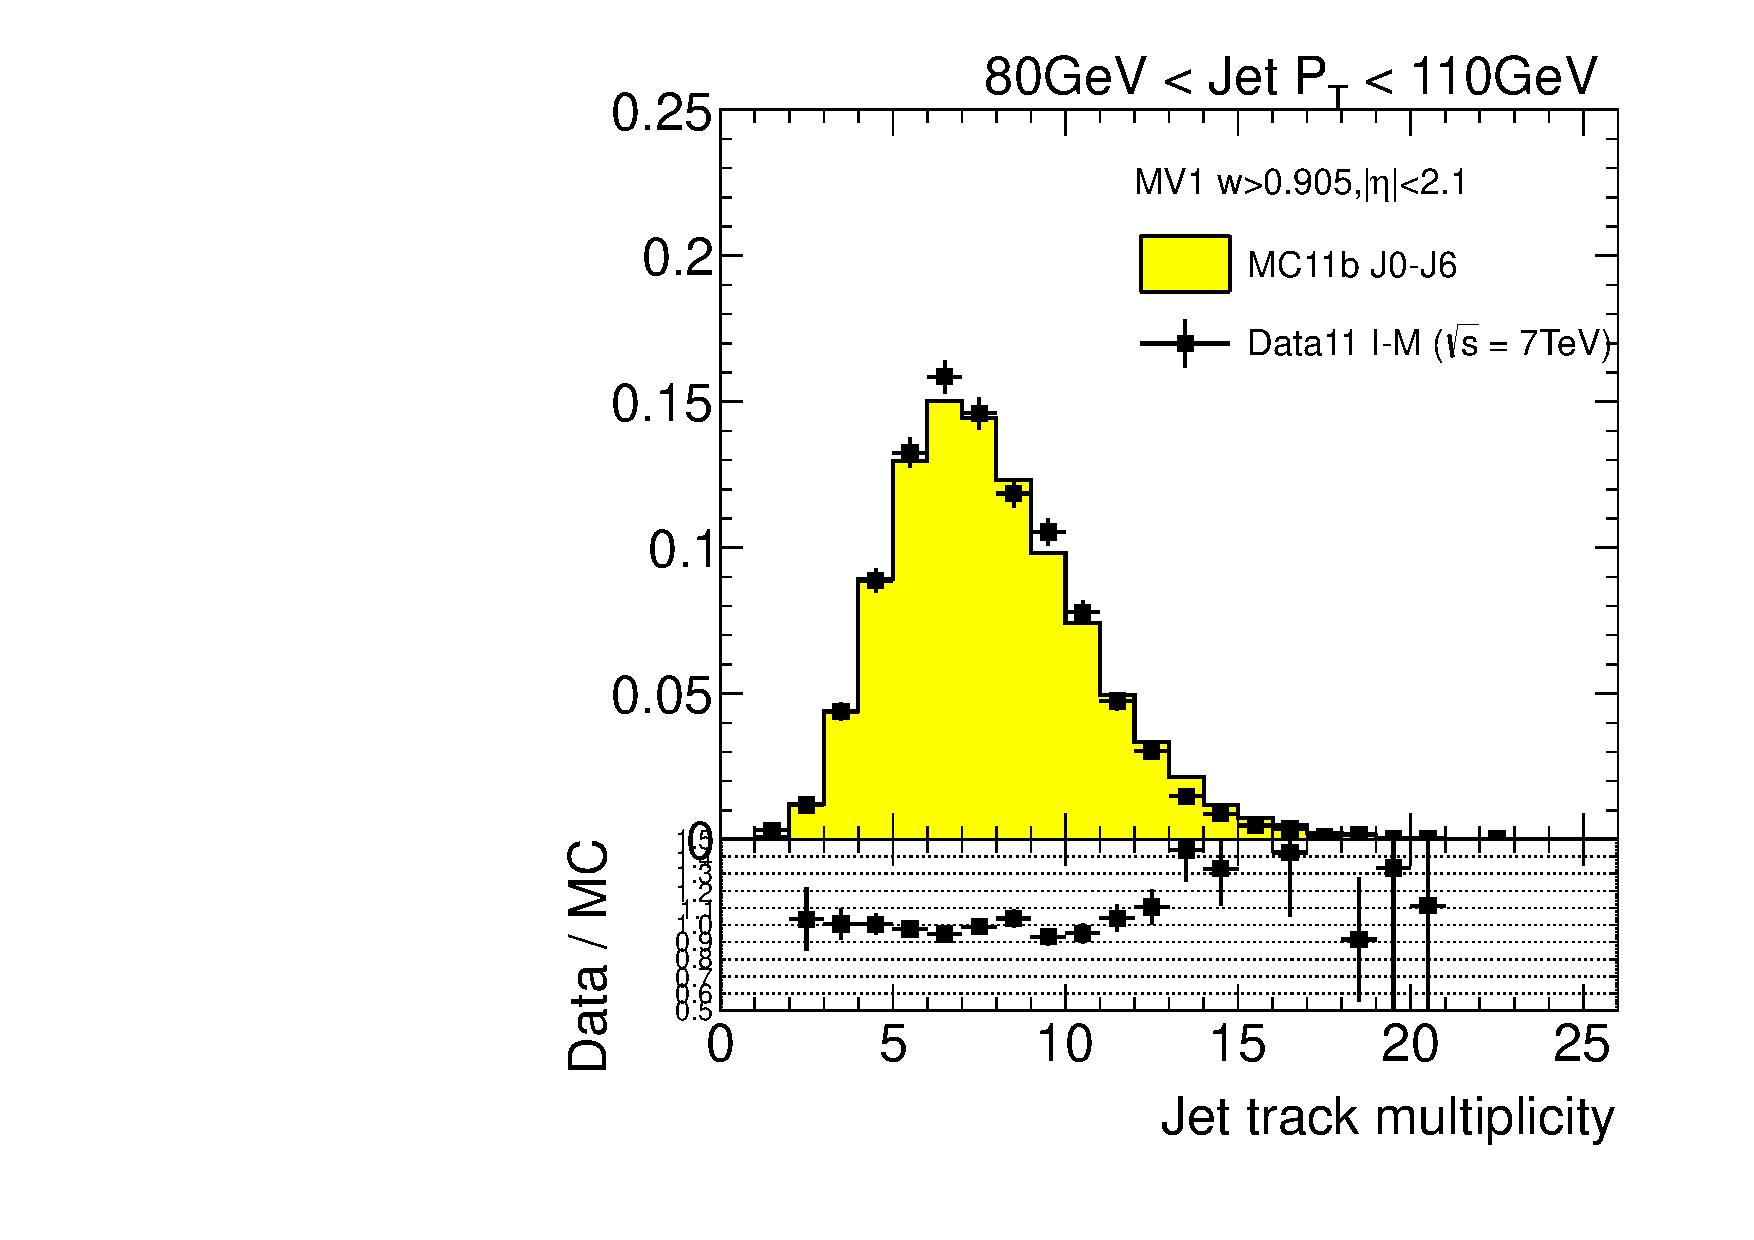
\includegraphics[width=0.49\textwidth]{FIGS/dataMCItoM/VarNtrkPT080.pdf}
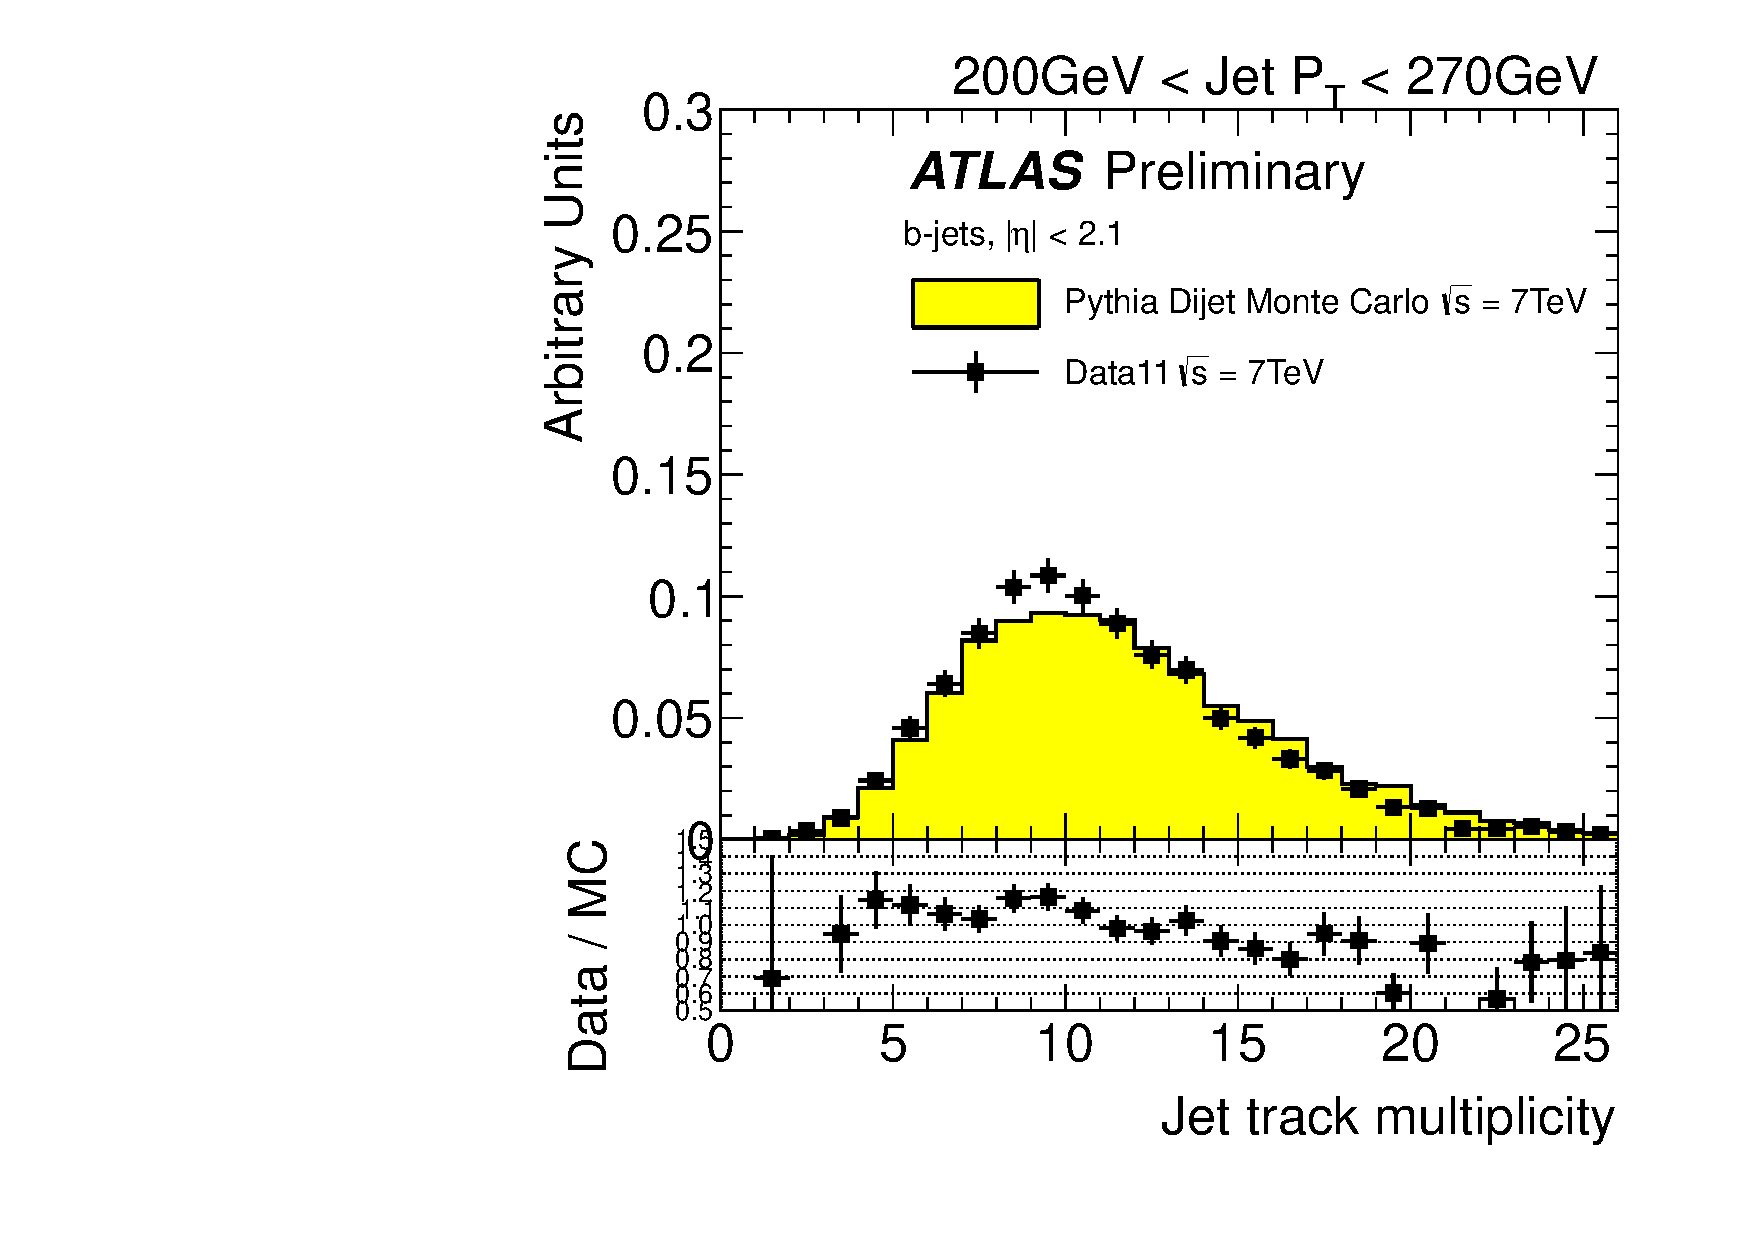
\includegraphics[width=0.49\textwidth]{FIGS/dataMCItoM/VarNtrkPT200.pdf}
\caption{ Distribution of the jet track-multiplicity in 2 different jet $\pt$ bins, for experimental data from data-taking periods I to M (solid black points) and simulated data (filled histograms). The ratio data\/simulation is shown at the bottom of the plot.}
\label{fig:datamcinputvarsItoM}
\end{figure}


%------------------------------------------------------------------------
\section{Multivariate Analysis}\label{sec:gbbTMVA}
%------------------------------------------------------------------------
A discriminant between single $b$-jets and merged $b$-jets was built by training a simple likelihood estimator in the context of the Toolkit for Multivariate Data Analysism, TMVA~\cite{Hocker:2007ht}.

A sub-set of the di-jet Monte Carlo sample was used for training. After the event and jet selections were performed, the jets with $|\eta| < 2.1$ and $w > 0.905$ were classified as signal (single $b$-jets) or background (merged $b$). % depending on whether one or two $B$-hadrons were found within a 0.4 cone around the jet axis. %For the evaluation of the method the same procedure was followed.
The likelihood training was done in bins of calorimeter jet $\pt$. % and only isolated jets were considered. 
Signal and background jets were not weighted by the dijet samples cross-sections to allow the contribution of subleading lower \pt\ jets from high \pt\ events, and thus increase the statistics of merged jets in the low \pt\ bins. For the evaluation of the method the same procedure was followed.

Several combinations of the tracking and jet shape variables studied in the previous section were tested as input variables. We found that $N_{\it trk}$, track-jet width and $\Delta {\rm R}_{k_{\rm T}}$ offer the best performance.

The distribution of the likelihood output for single and merged $b$-jets is shown in  Fig.~\ref{fig:outputinbins} for three different bins of calorimeter jet $\pt$.

\begin{figure}[tp]
\centering
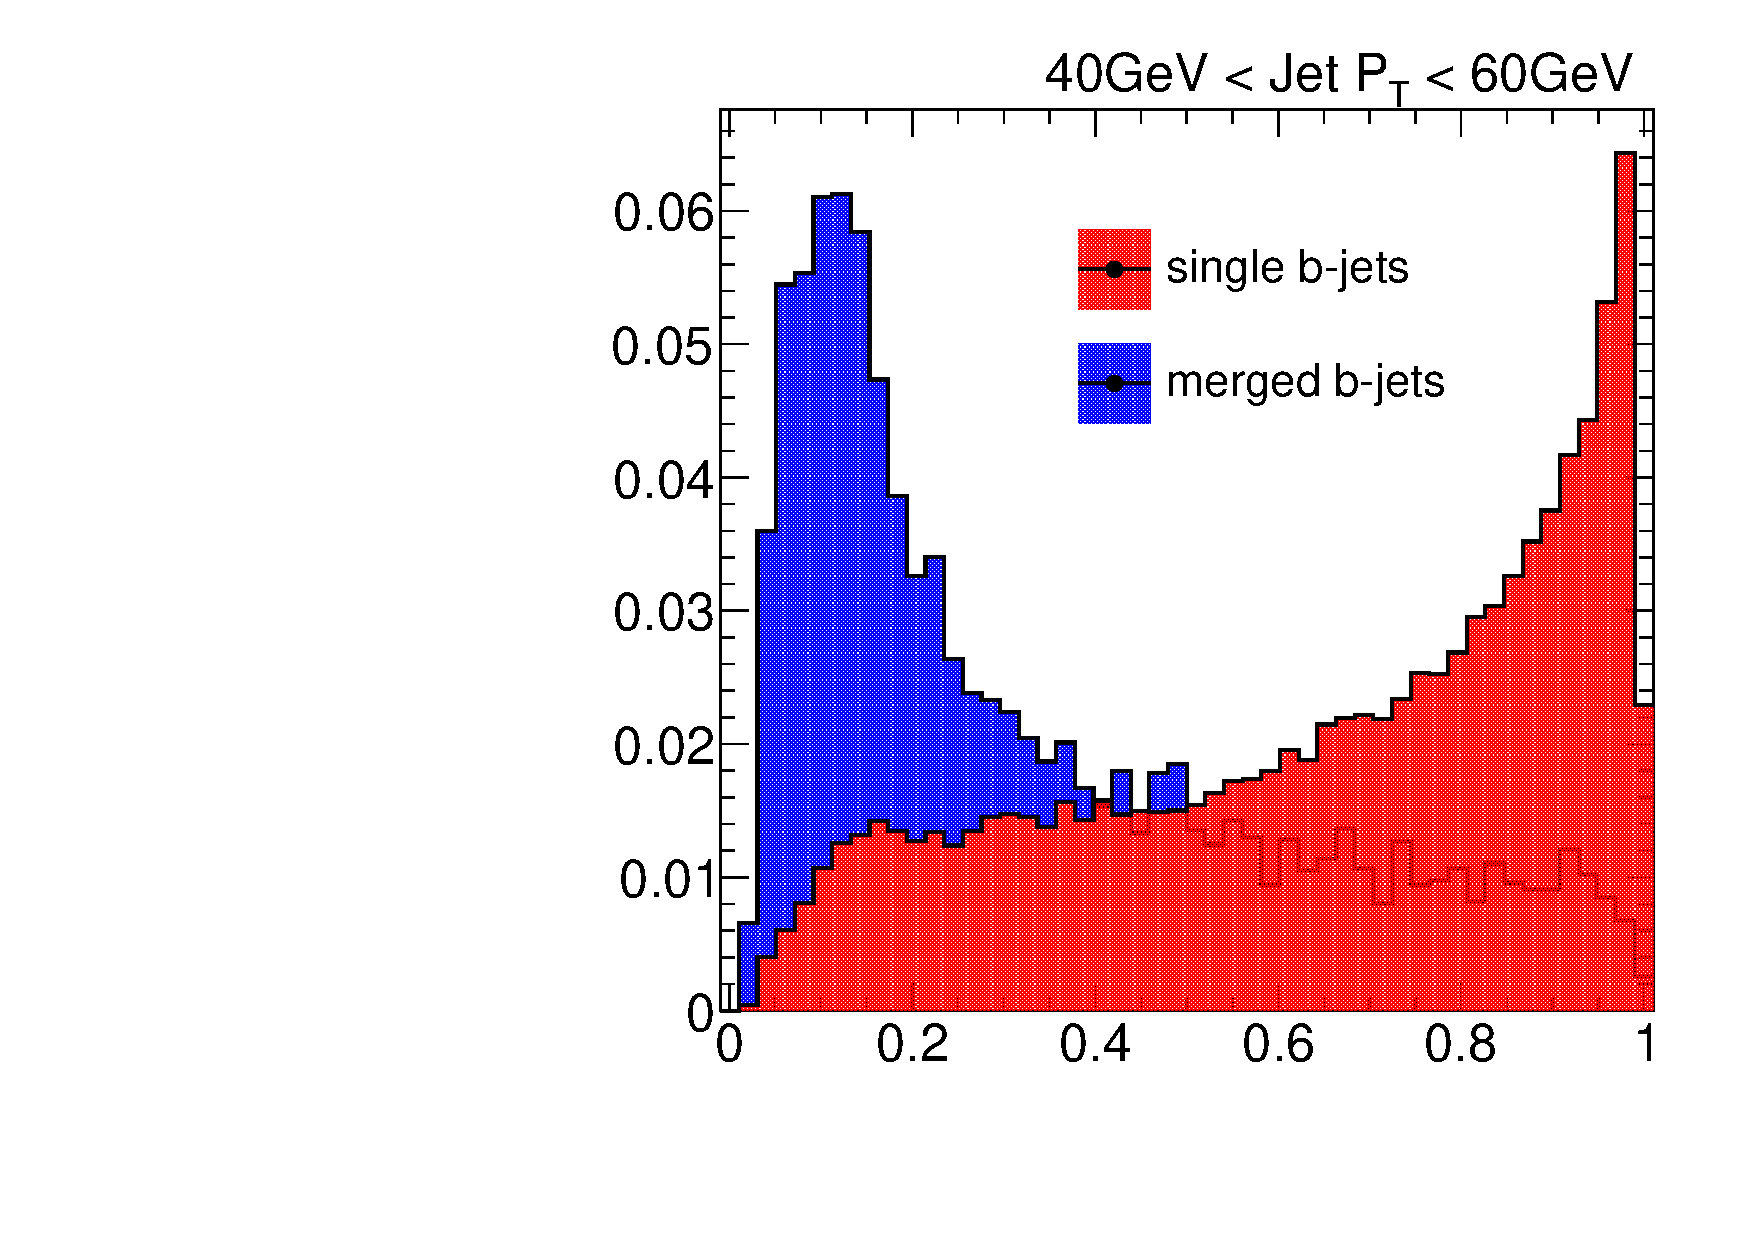
\includegraphics[width=0.32\textwidth,viewport=35 45 540 550,clip]{FIGS/Likelihood/NNoutput040_LihoodKDE.pdf}
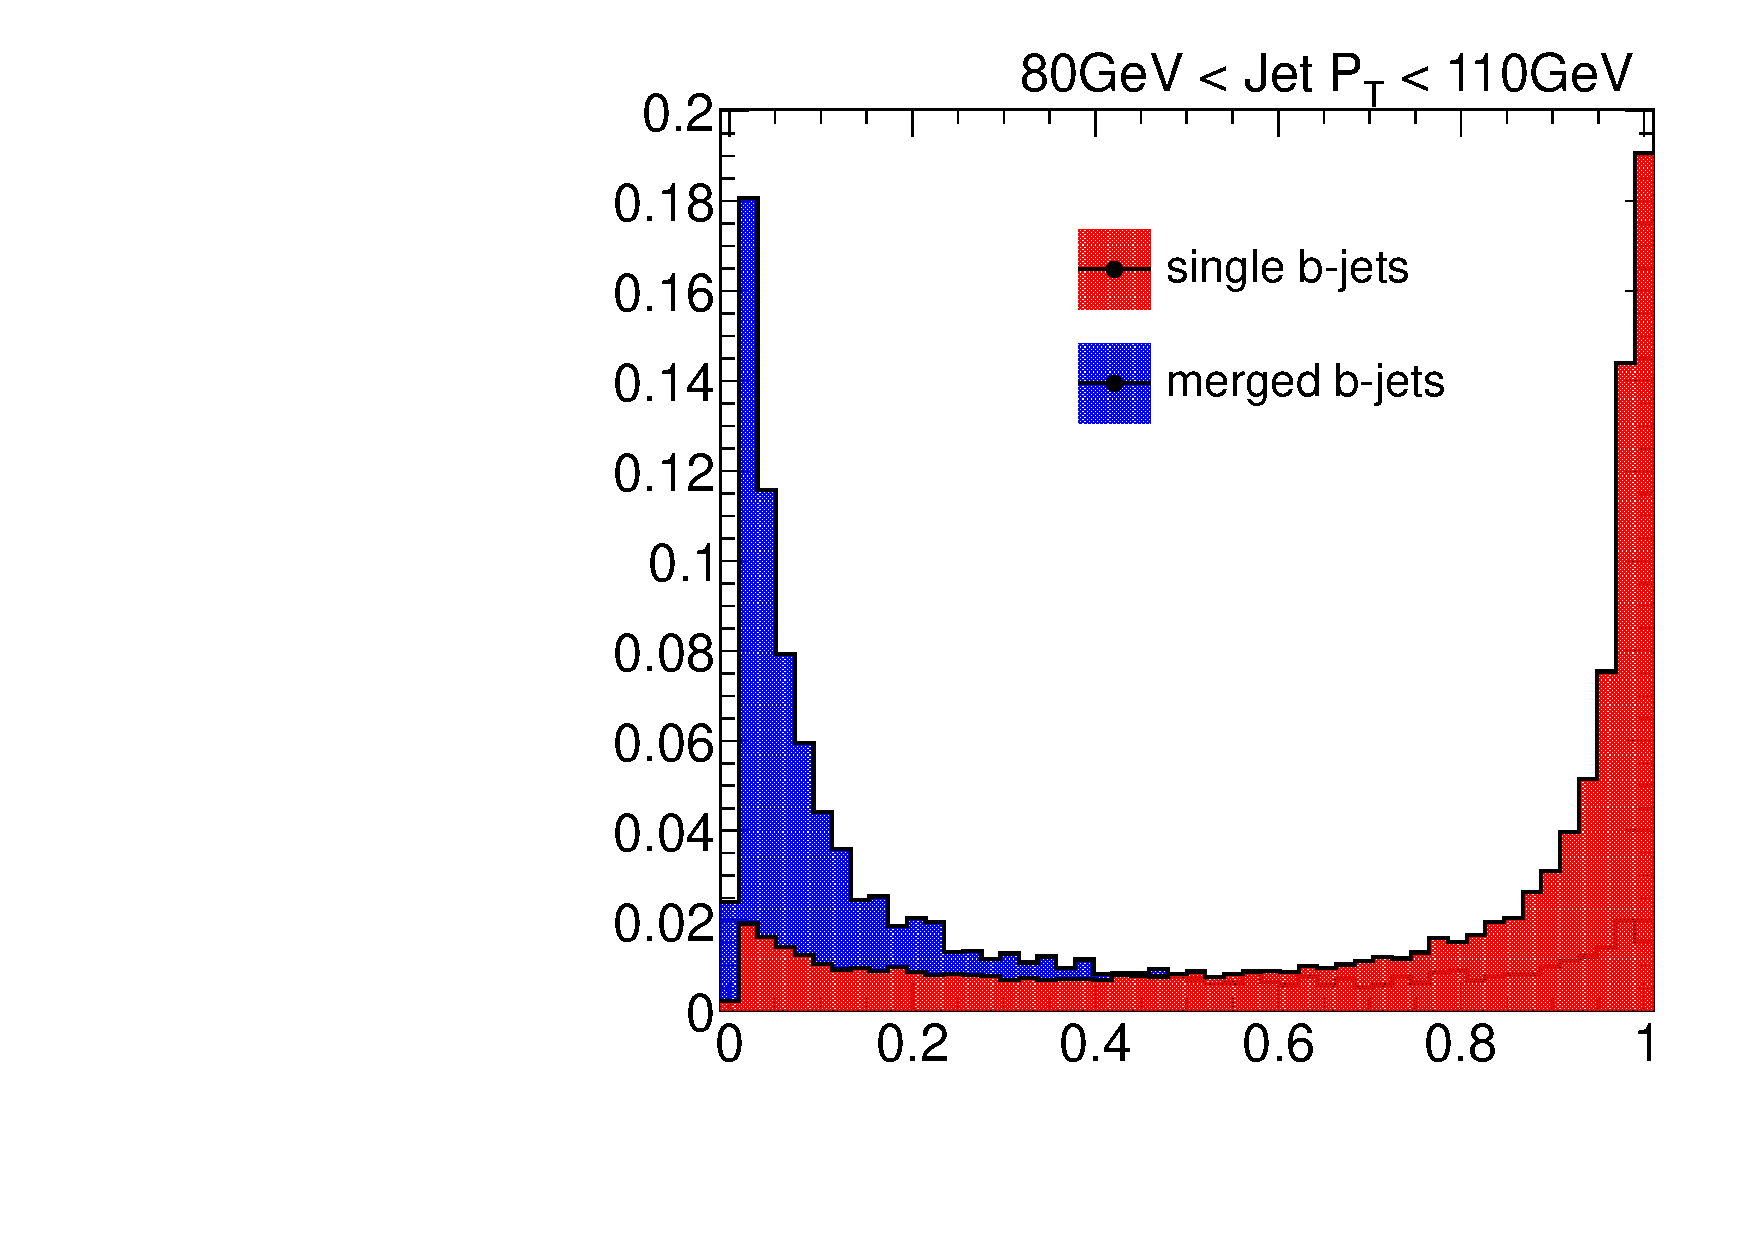
\includegraphics[width=0.32\textwidth,viewport=35 45 540 550,clip]{FIGS/Likelihood/NNoutput080_LihoodKDE.pdf}
%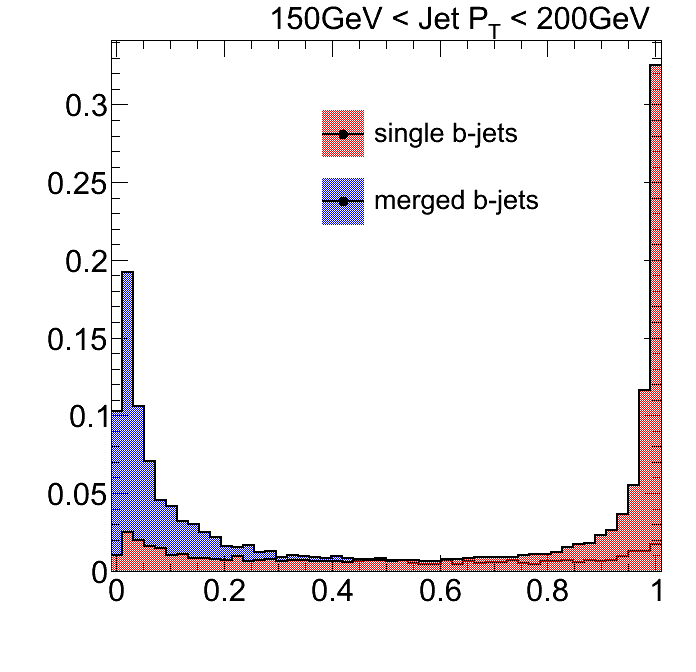
\includegraphics[width=0.49\textwidth,viewport=45 45 696 672,clip]{FIGS/Likelihood/NNoutput150_LihoodKDE.png}
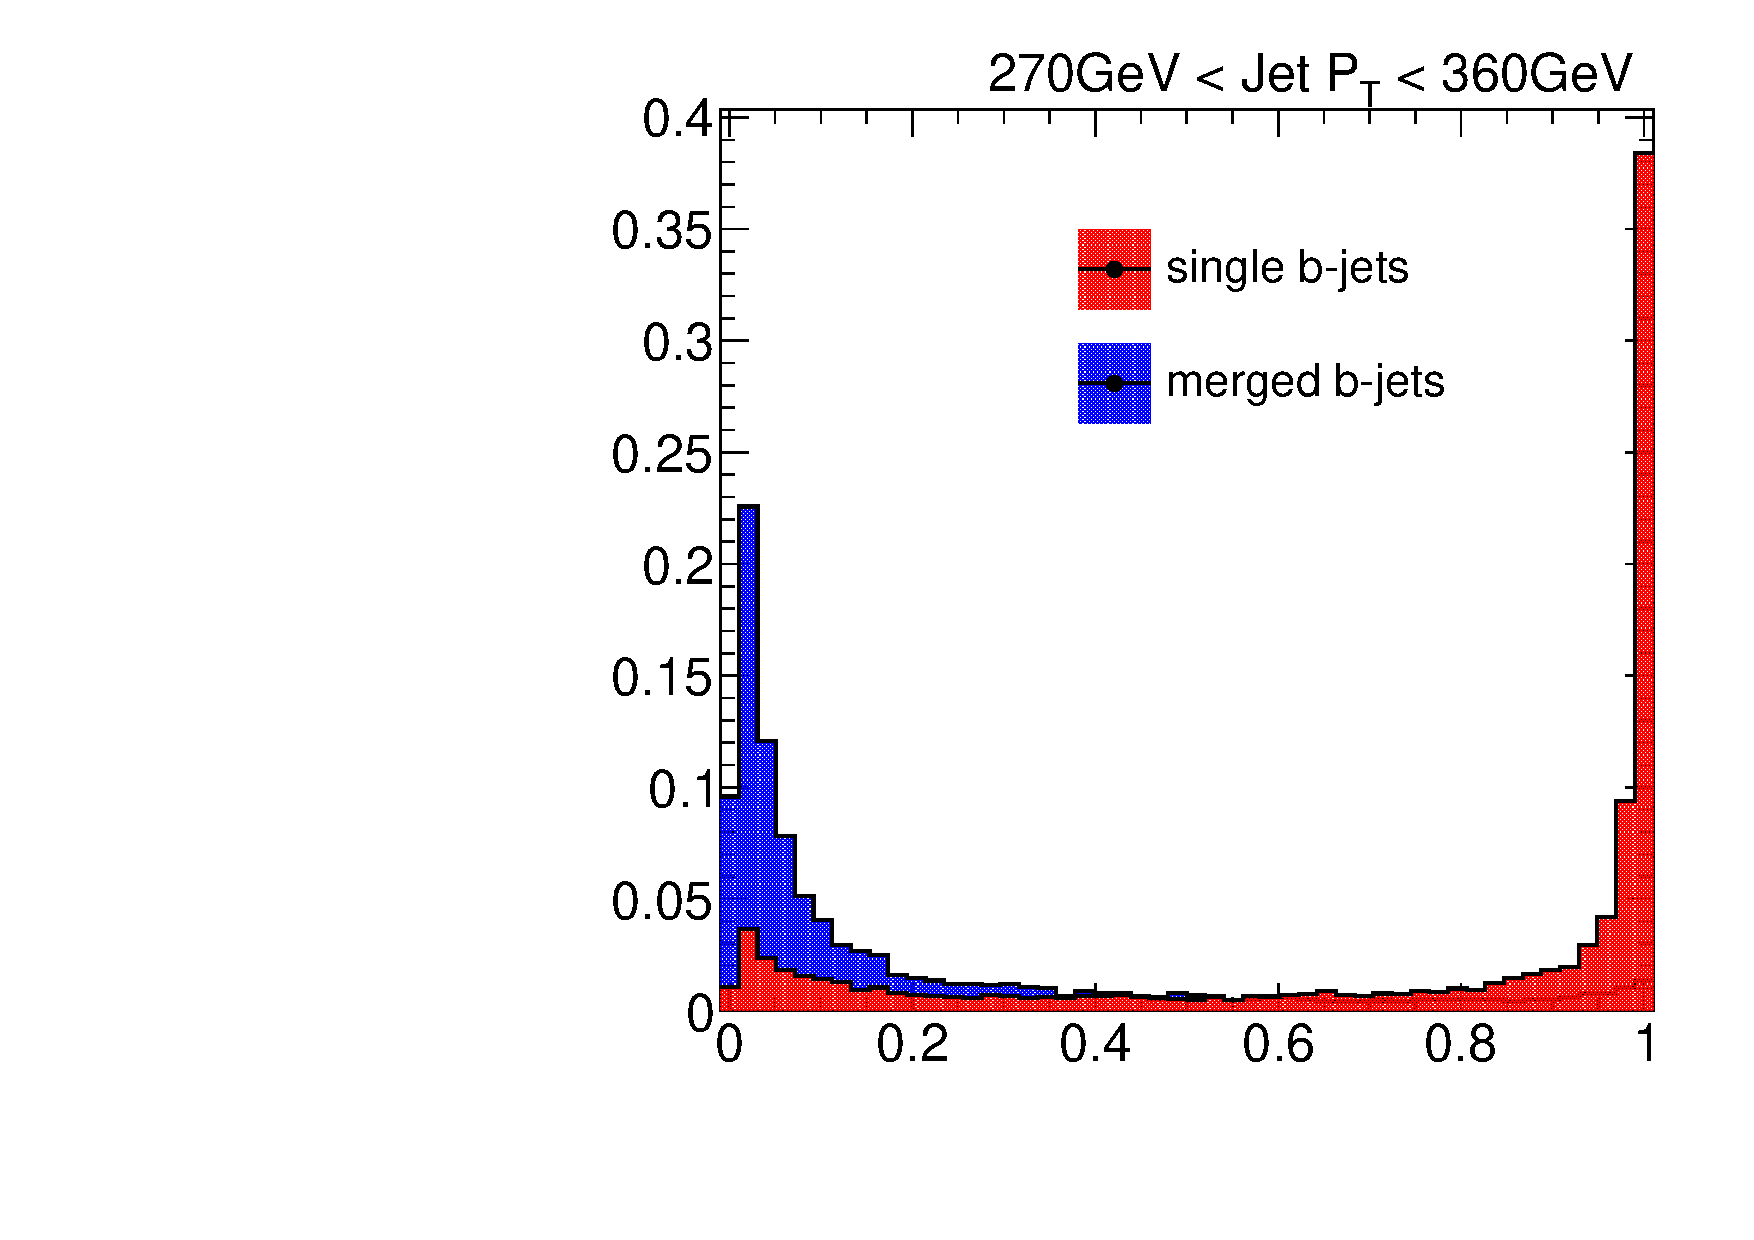
\includegraphics[width=0.32\textwidth,viewport=35 45 540 550,clip]{FIGS/Likelihood/NNoutput270_LihoodKDE.pdf}  
\caption{Distribution of the $g\rightarrow b \bar{b}$ likelihood output for single and merged $b$-jets for different jet $\pt$ bins.}
\label{fig:outputinbins}
\end{figure}

The performance of the $g\rightarrow b \bar{b}$ tagger in the simulation can be seen in Fig.~\ref{fig:performanceinbins}. In this plot the rejection ($1/\epsilon_{bkg}$) of merged $b$-jets from gluon splitting is shown as a function of single $b$-jet efficiency for the eight bins of jet $\pt$ mentioned in section~\ref{sec:EventSelection}. The performance improves with $\pt$:


\begin{itemize}\addtolength{\itemsep}{-0.4\baselineskip}
\item
$\pt>40$ GeV: %\\[1mm]
 over 85\% rejection at 50\% eff.
\item
$\pt>60$ GeV: %\\[1mm]
 90\% rejection at 50\% eff.
\item
$\pt>150$ GeV: %\\[1mm]
 over 95\% rejection at 50\% eff.
\end{itemize}


\begin{figure}[tp]
\centering
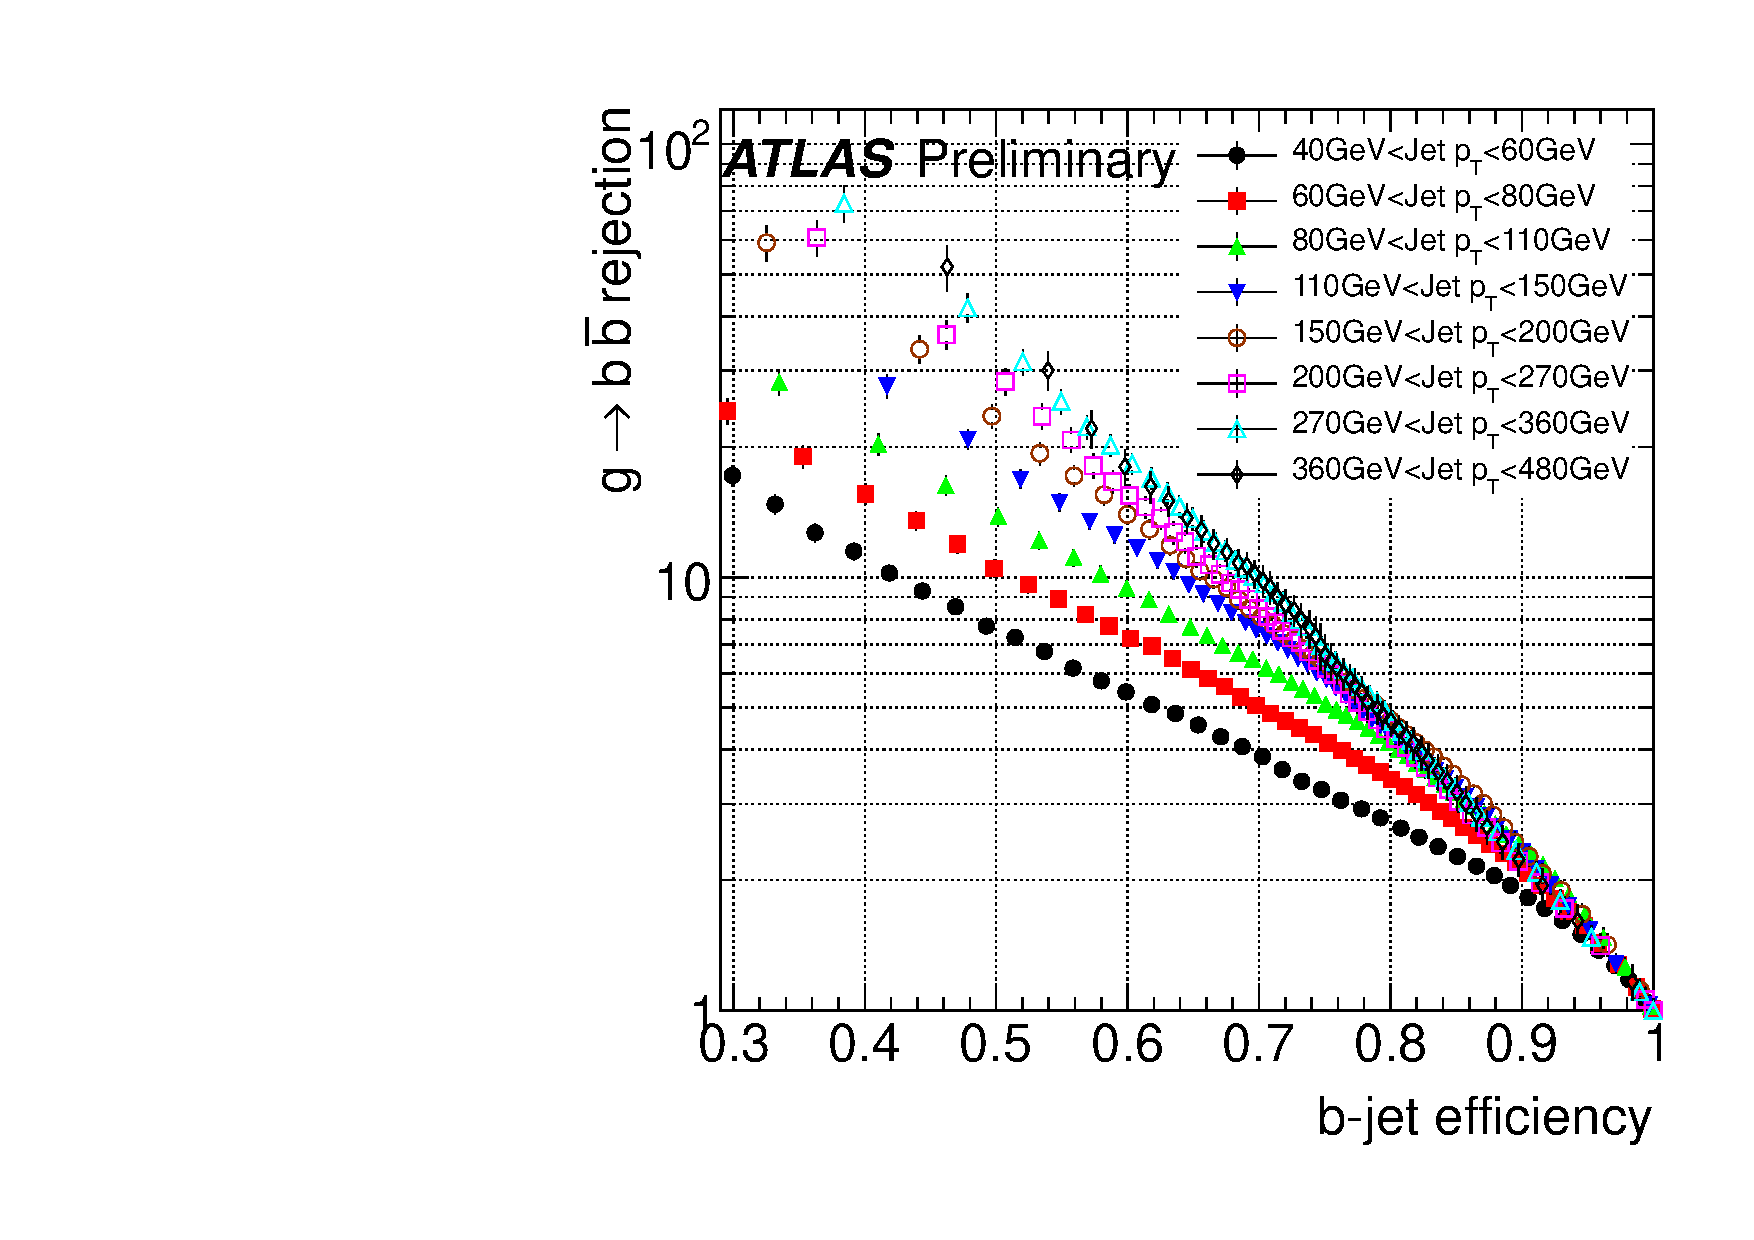
\includegraphics[width=0.7\textwidth]{FIGS/Likelihood/KDE_RejvsEff.pdf}
\caption{Rejection of $g\rightarrow b \bar{b}$ merged b-jets as a function of $b$-jet efficiency for dijet events in 8 jet $\pt$ bins.}
\label{fig:performanceinbins}
\end{figure}

The likelihood was trained with jets that had been first tagged by the MV1 algorithm. In order to use the  $g\rightarrow b \bar{b}$ classifier for jets tagged by another tagger a new training is required.

The rejection of merged jets attained as a function of \pt\ for the 50\% and 60\% efficiency working points are summarized in Table~\ref{tb:rejection}, together with their relative statistical error. These are propagated from the Poisson fluctuations of the number of events in the merged and single $b\bar{b}$ distributions. The error is slightly lower for the 60\% efficiency working point because a higher efficiency allows for a greater number of Monte Carlo events to measure the performance. %the higher the efficiency, the larger the number of Monte Carlo events available to measure the performance.

%Although the tagger was derived with isolated jets it can also be applied to non-isolated jets. Studies were performed to evaluate the likelihood rejection in $b$-jets with close-by jet with $\pt$ between 7 GeV at electromagnetic scale scale and 90$\%$ of the $b$-jet $\pt$. The results can be seen in  Fig.~\ref{fig:testisolation}. The presence of close-by jets with a susbtancial fraction of the $b$-jet pt worsens the performance in more than 50$\%$ at very high $\pt$. 

%\begin{figure}[tp]
%\centering
%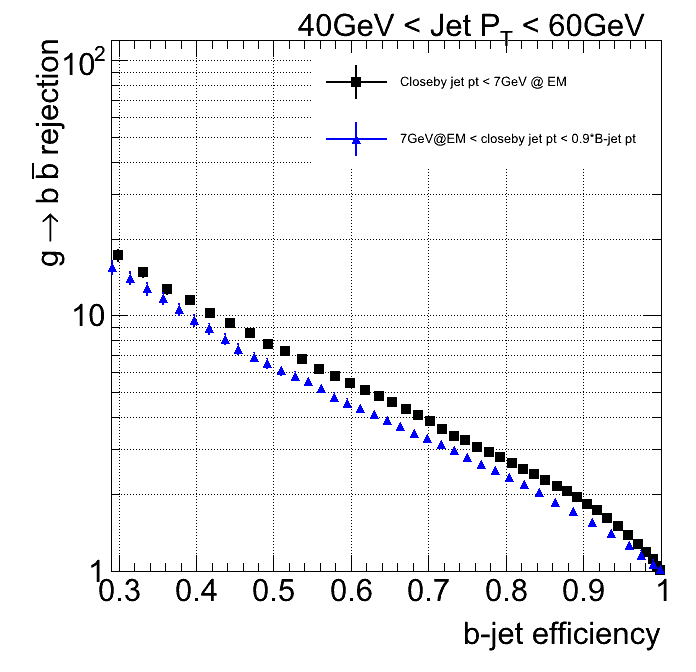
\includegraphics[width=0.4\textwidth]{FIGS/systematics/DiffIsolationCutsKDE_RejvsEff40.png}
%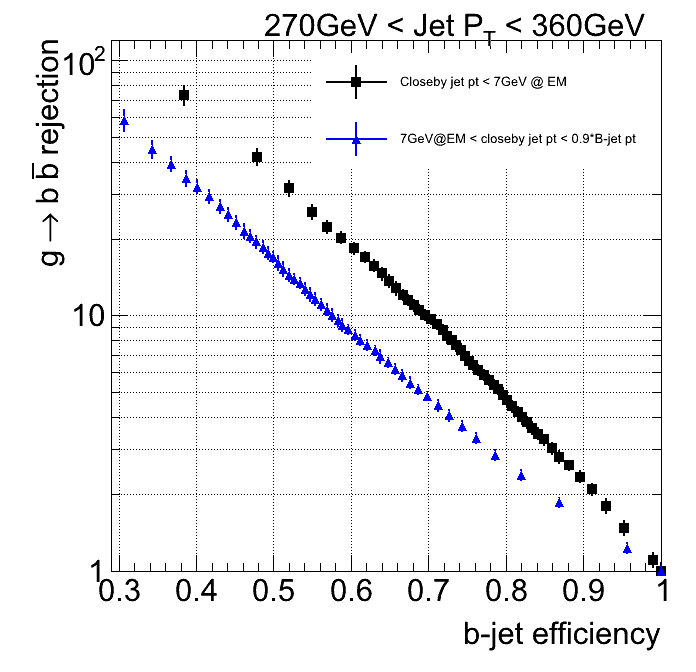
\includegraphics[width=0.4\textwidth]{FIGS/systematics/DiffIsolationCutsKDE_RejvsEff270.png}
%\caption{Rejection of $g\rightarrow b \bar{b}$ merged b-jets as a function of $b$-jet efficiency for two different isolation cuts.}
%\label{fig:testisolation}
%\end{figure}


%\begin{table}[!hbt] %[h]
%\renewcommand{\arraystretch}{1.2}
%\centering
%\begin{tabular}{ | c || c | c || c | c||}
%  \hline
%  Jet \pt & \multicolumn{2}{c||}{Efficiency 50\%} & 
%            \multicolumn{2}{c||}{Efficiency 60\%}\\ \cline{2-5}
%    (GeV )  & Rejection & ~stat.err.~ & Rejection & ~stat.err.~ \\ \hline
%   40 - 60 &  ~7.6 &  4\%  &  ~5.4  &  3\%    \\ 
%   60 - 80 &  10.6 &  4\%  &  ~7.3  &  4\%    \\ 
%   80 - 110&  14.0 &  5\%  &  ~9.4  &  4\%    \\ 
%  110 - 150&  18.7 &  5\%  &  12.0  &  4\%    \\ 
%  150 - 200&  23.8 &  5\%  &  14.0  &  5\%    \\ 
%  200 - 270&  28.9 &  7\%  &  15.6  &  6\%    \\ 
%  270 - 360&  35.3 &  7\%  &  18.7  &  6\%    \\ 
%  360 - 480&  39.4 &  8\%  &  18.2  &  8\%    \\ \hline
%\end{tabular}
%\caption{The merged $b$-jet rejection for the 50\% and 60\% efficiency working points in bins of $\pt$.}
%\label{tb:rejection}
%\end{table}


%------------------------------------------------------------------------
\section{Systematic uncertainties}\label{sec:gbbSystematics}
%------------------------------------------------------------------------
The development, training and performance determination of the tagger is based on simulated events. Although the agreement between simulation and data explored in section~\ref{sec:validation} is a necessary validation condition, it is important to investigate how the tagger performance depends on relevant systematics in the data. In particular we have considered:
%
%There are uncertainties in the data that, although not spoiling the data/MC agreement, might change the performance of the tagger. This uncertainties would also be present in an eventual future data-driven determination of the performance as  the data are not known better that this.The following systematic effects have been studied and their influence on the tagger performance ascertained:
%
%In order to study the systematic uncertainties in the method the following contributions were evaluated:
\begin{itemize}\addtolength{\itemsep}{-0.4\baselineskip}
\item
presence of additional interactions (pile-up)
\item
uncertainty in the $b$-jet tagging efficiency % and b-jet energy scale?
\item
uncertainty in the track reconstruction efficiency
\item
uncertainty in the track transverse momentum resolution
\item
uncertainty in the jet transverse momentum resolution  
%\item
%the effect of jet isolation
%\item
%other $\Delta R$ cuts for B-labeling and matching
\end{itemize}

{ \em I. Pile-up}
\\[3mm]
  The size of this effect was studied by comparing the performance of the likelihood discriminant with $b$-jets in events with small (1-9) and large (9-20) number of primary vertices. 
%The comparison of the performance in these two sub-samples can be seen in Fig.~\ref{fig:performanceinbinsMu}. 
As expected from the use of tracking (as opposed to calorimeter) variables no significant dependence with pile-up is observed within statistics. Of the 20 determinations (2 working points with 10 \pt\ bins each) of performance differences between high and low number of primary vertices events, it is observed that 12 of them are positive and 8 negative, with a global mean of 0.3\%. We conclude that the effect is negligible compared to other source of uncertainties.
%

%\begin{figure}[tp]
%\centering
%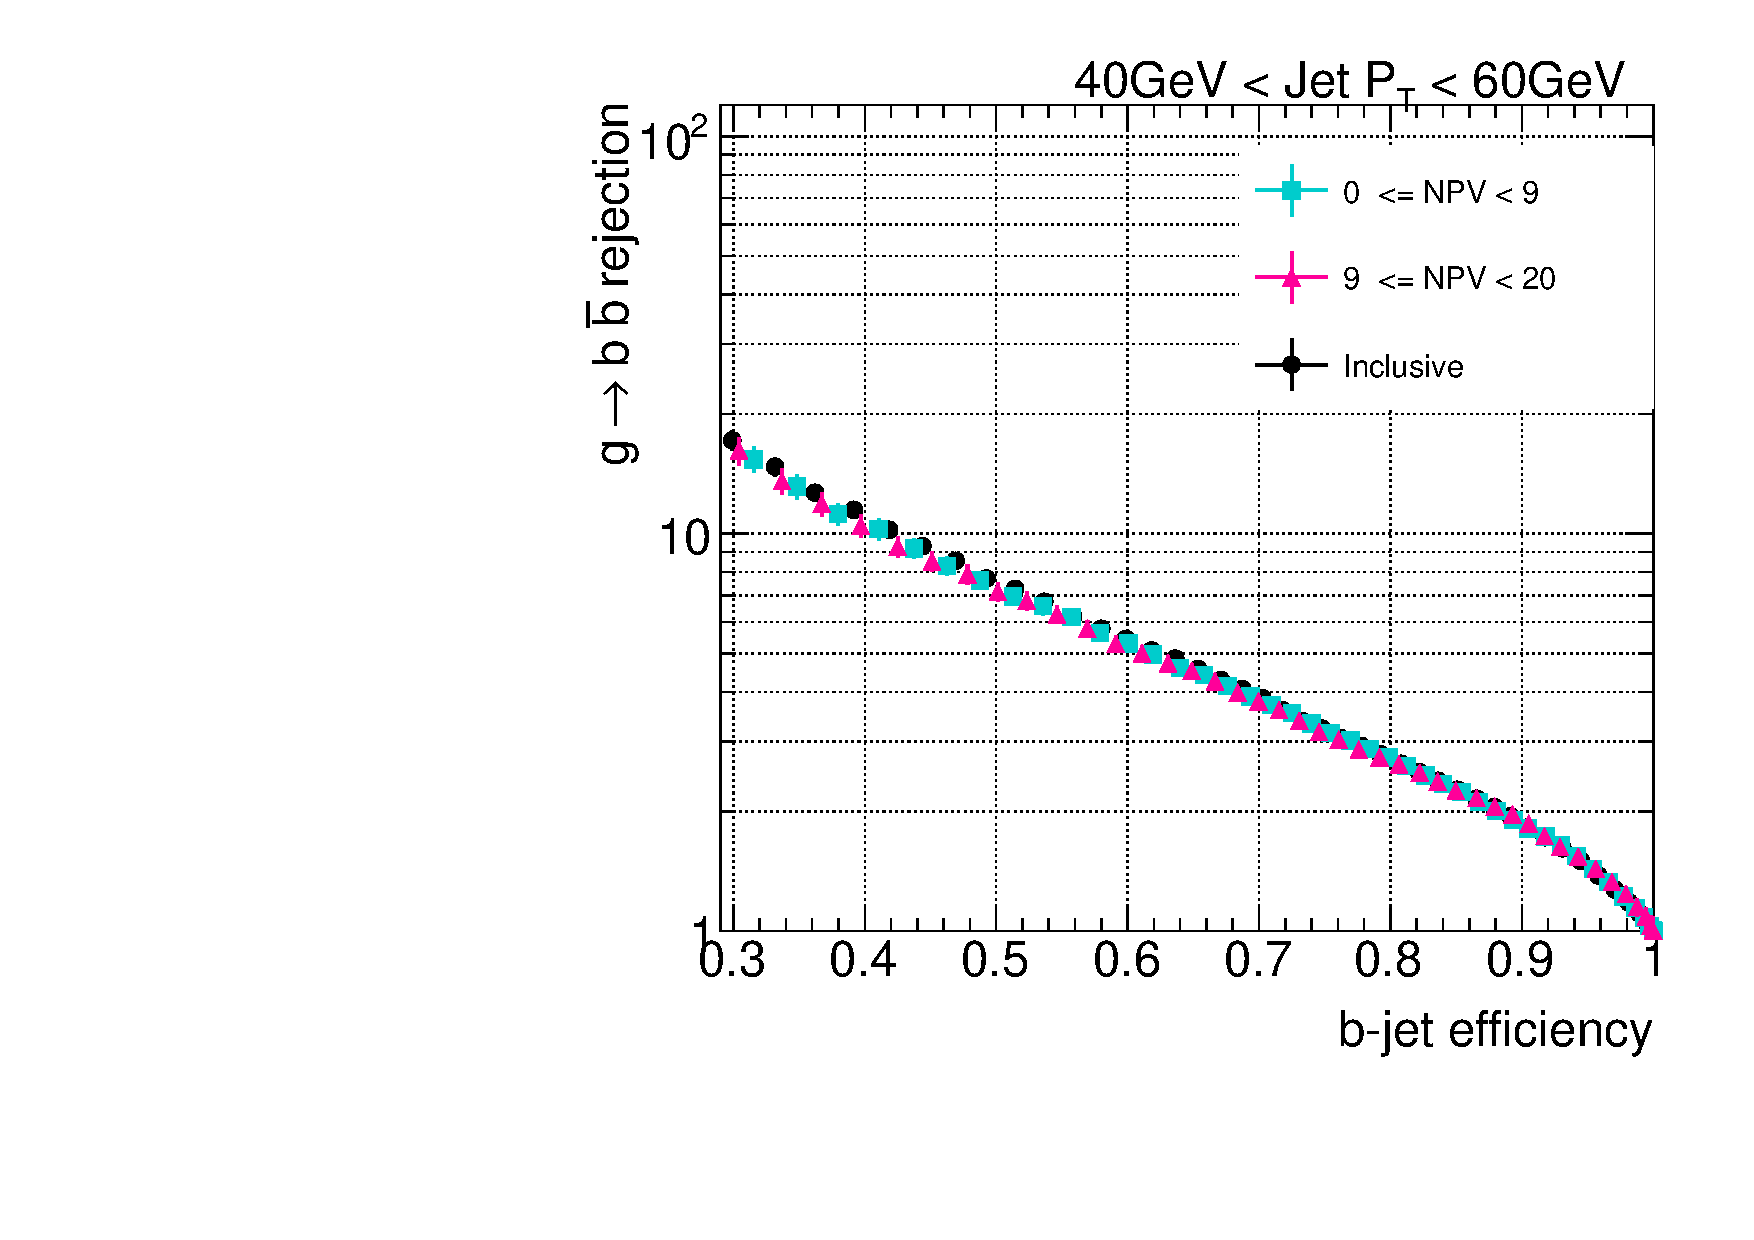
\includegraphics[width=0.49\textwidth]{FIGS/systematics/50BinsLlhoodKDE_ISO_PileUp_rejvseff040.pdf}
%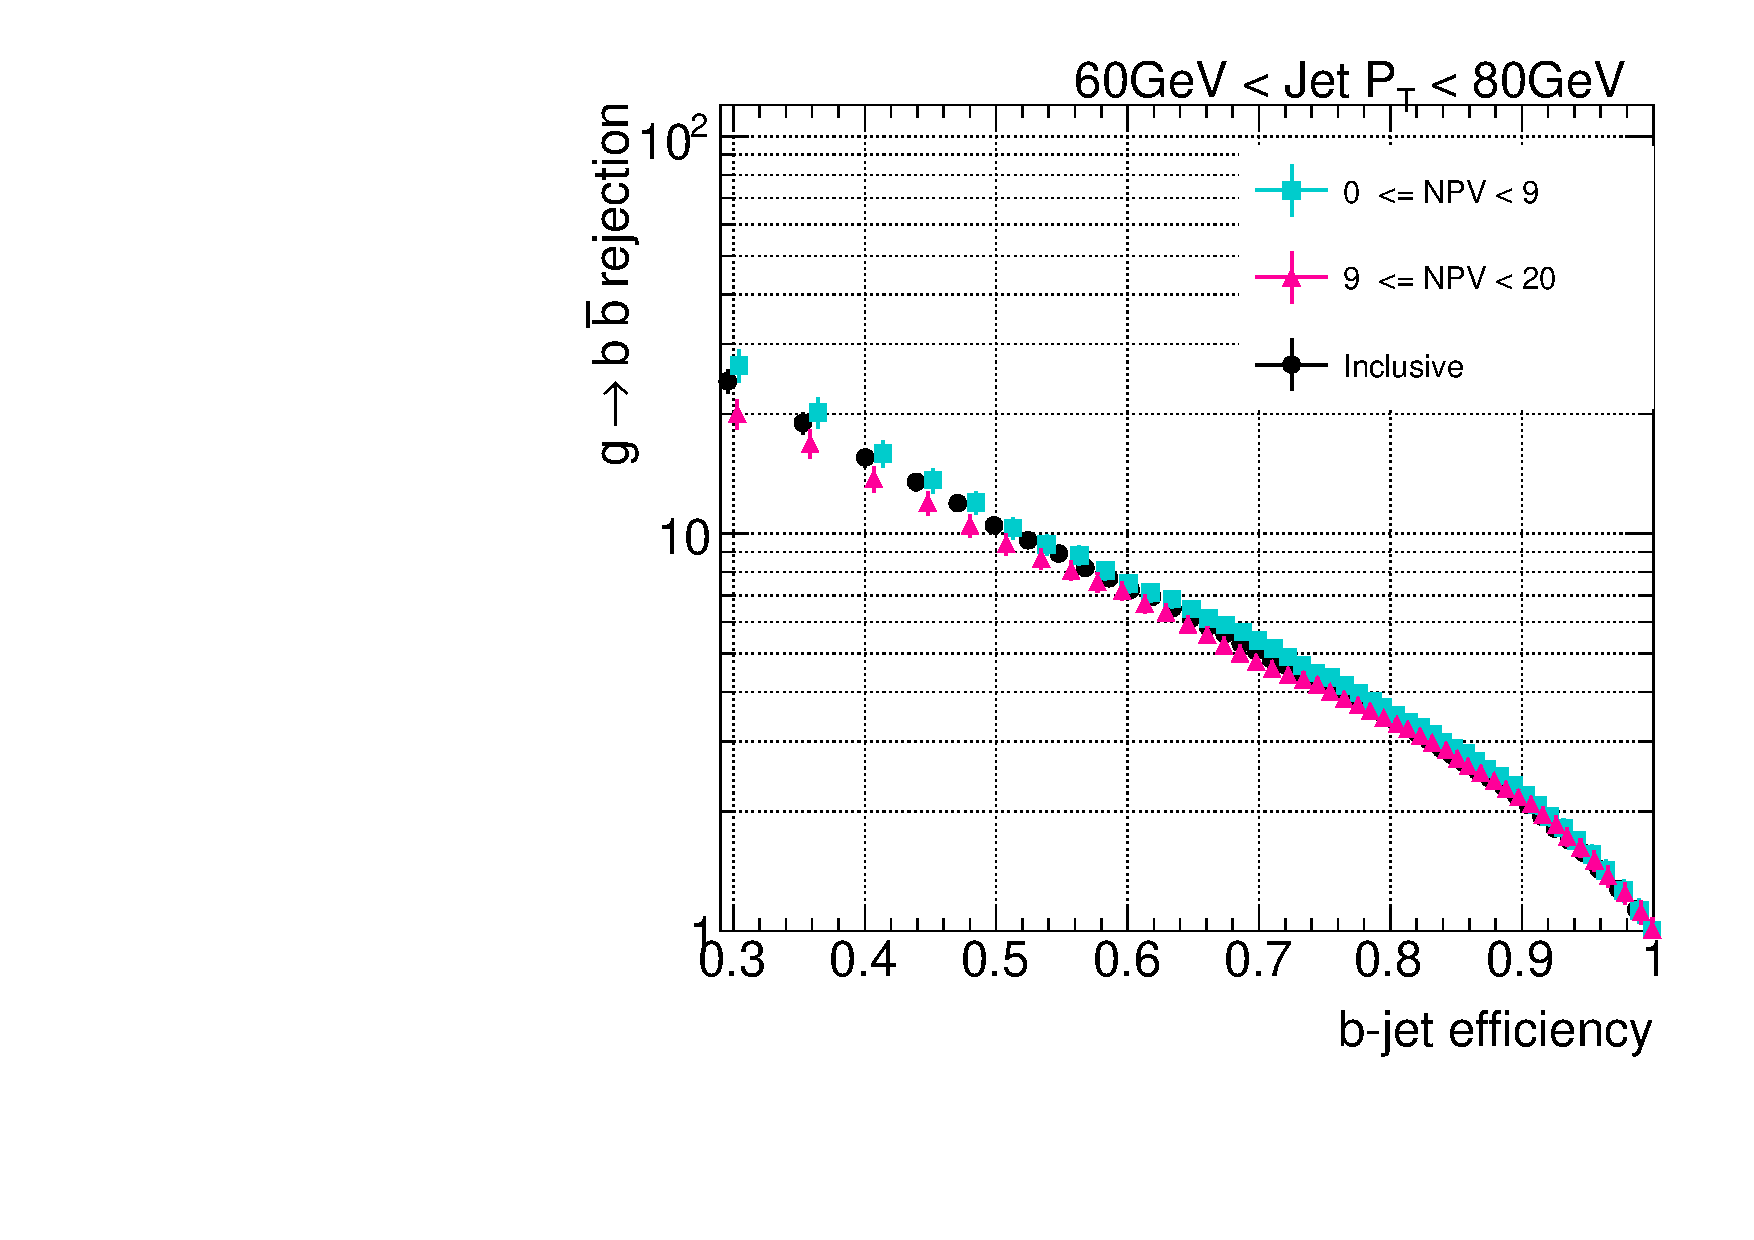
\includegraphics[width=0.49\textwidth]{FIGS/systematics/50BinsLlhoodKDE_ISO_PileUp_rejvseff060.pdf}
%\caption{Rejection of $g\rightarrow b \bar{b}$ merged b-jets as a function of $b$-jet efficiency in bins of $N_{\rm vtx}$ for two low jet $\pt$ bins.}
%\label{fig:performanceinbinsMu}
%\end{figure}

\vspace{3mm}
{\em II. b-tagging efficiency} %energy scale and 
\\[3mm]
The performance of heavy-flavor tagging in Monte Carlo events is calibrated to experimental data by means of the scale factors (SFs) measured by the $b$-tagging group. %scale factors defined as the ratio of the heavy-flavor tagging efficiency in data over that in Monte Carlo (MC) for the different jet flavors, and probably also as a function of jet pT and η 
Such a measurement carries a systematic uncertainty, and in order to estimate its effect a conservative approach is followed: %https://twiki.cern.ch/twiki/bin/viewauth/AtlasProtected/BTaggingCalibrationDataInterface
the SFs are varied in all the $\pt$ bins simultaneously by one standard deviation both in the up and down directions. The result of this procedure for the distribution of the tracking variables used as discriminant is illustrated in Fig.~\ref{fig:btaggingSFs}. 

The effect of the $b$-tagging calibration uncertainty on the likelihood peformance is negligible.
% as it can be seen in Fig.~\ref{fig:btaggingSFsPerf}.
This was indeed expected. The scale factors depend on the true flavor of the jet and on its \pt, but these are basically constant in the performance determination, which is based on single flavor (true $b$-) jets classified in \pt-bins.

%\textwidth,viewport=45 45 696 672,clip
\begin{figure}[tp]
\centering
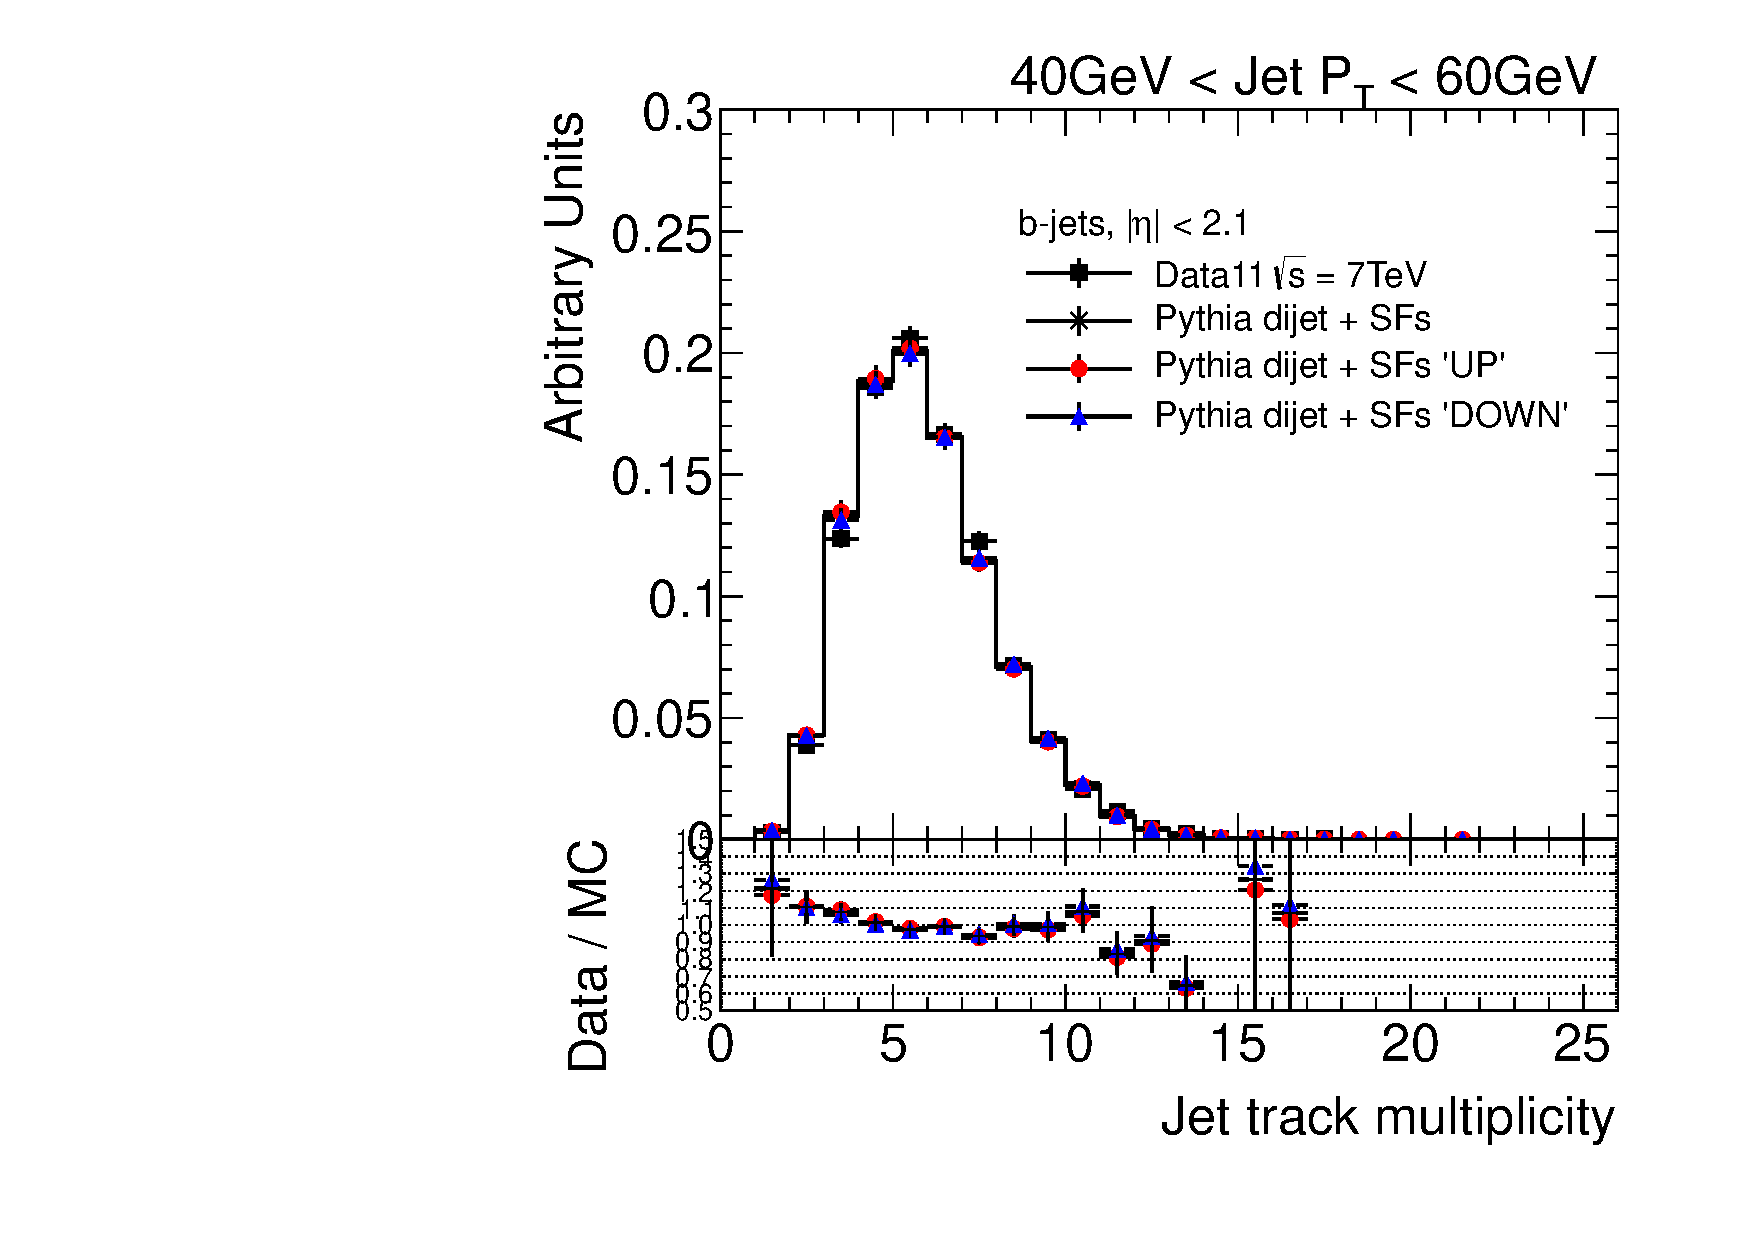
\includegraphics[width=0.49\textwidth]{FIGS/systematics/BTagCalib_DataVarNtrkPT040.pdf}
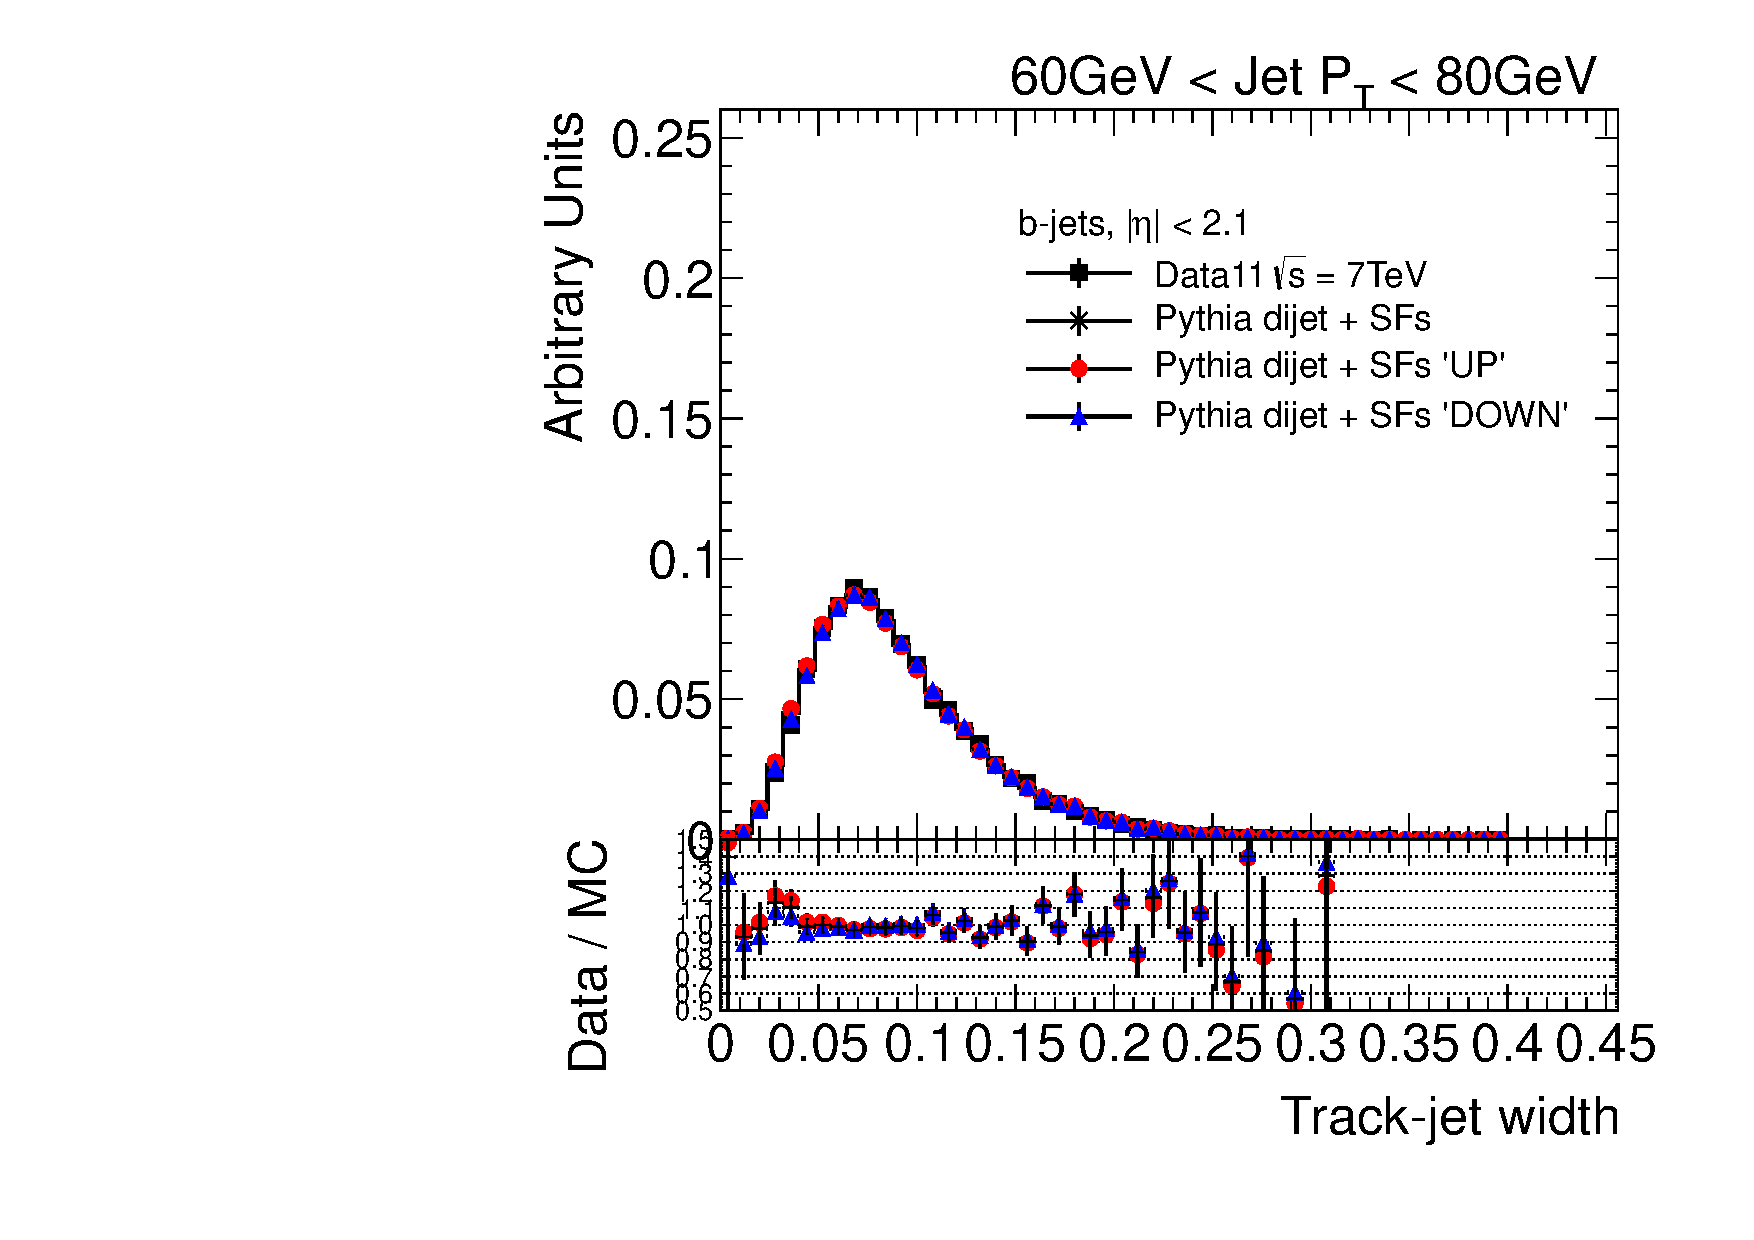
\includegraphics[width=0.49\textwidth]{FIGS/systematics/BTagCalib_DataVarTrkWidthPT060.pdf}
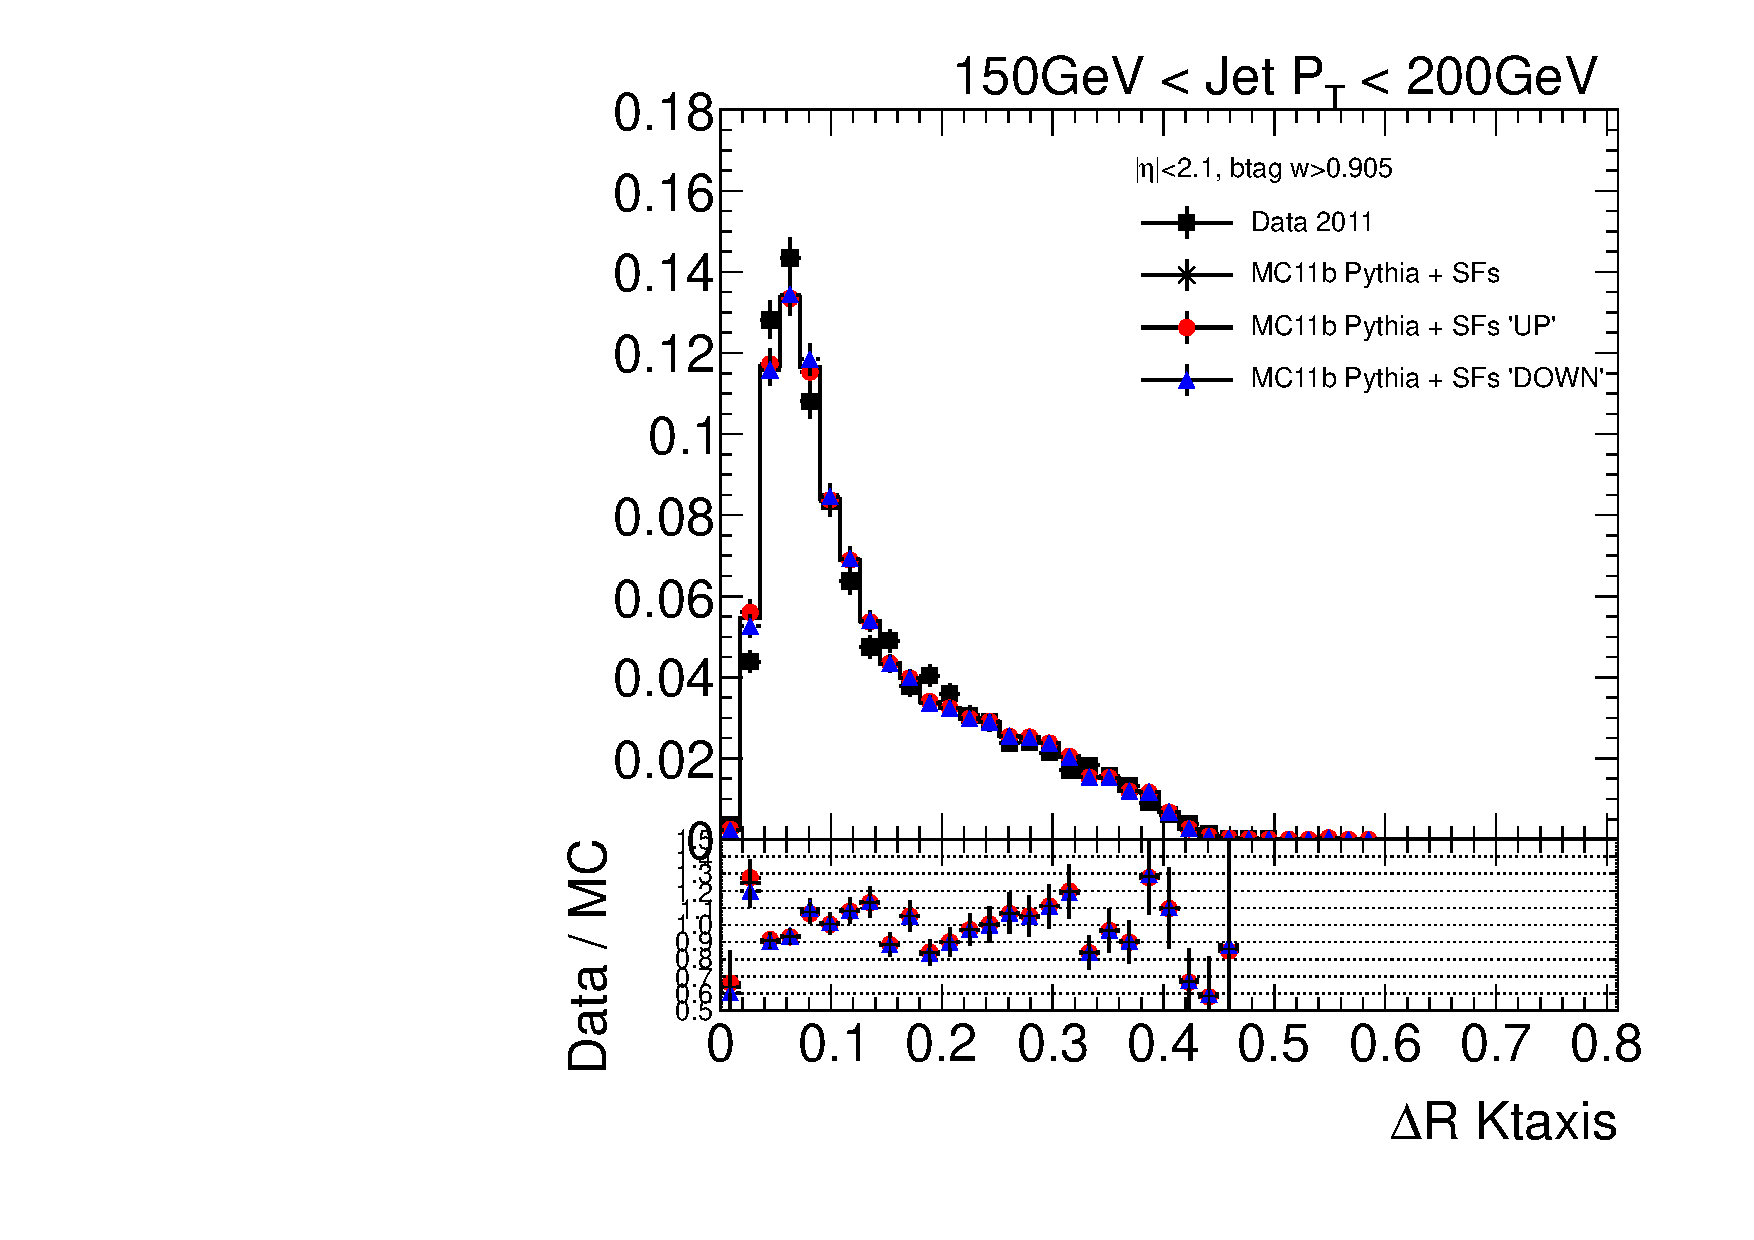
\includegraphics[width=0.49\textwidth]{FIGS/systematics/BTagCalib_DataVarDRktaxisPT150.pdf}
\caption{The effect of a variation in the $b$-tagging scale factors on the tracking variables distributions. SFs were varied up (down) by 1-sigma to evaluate the systematic uncertainty from this source.}
\label{fig:btaggingSFs}
\end{figure}

%\begin{figure}[tp]
%\centering
%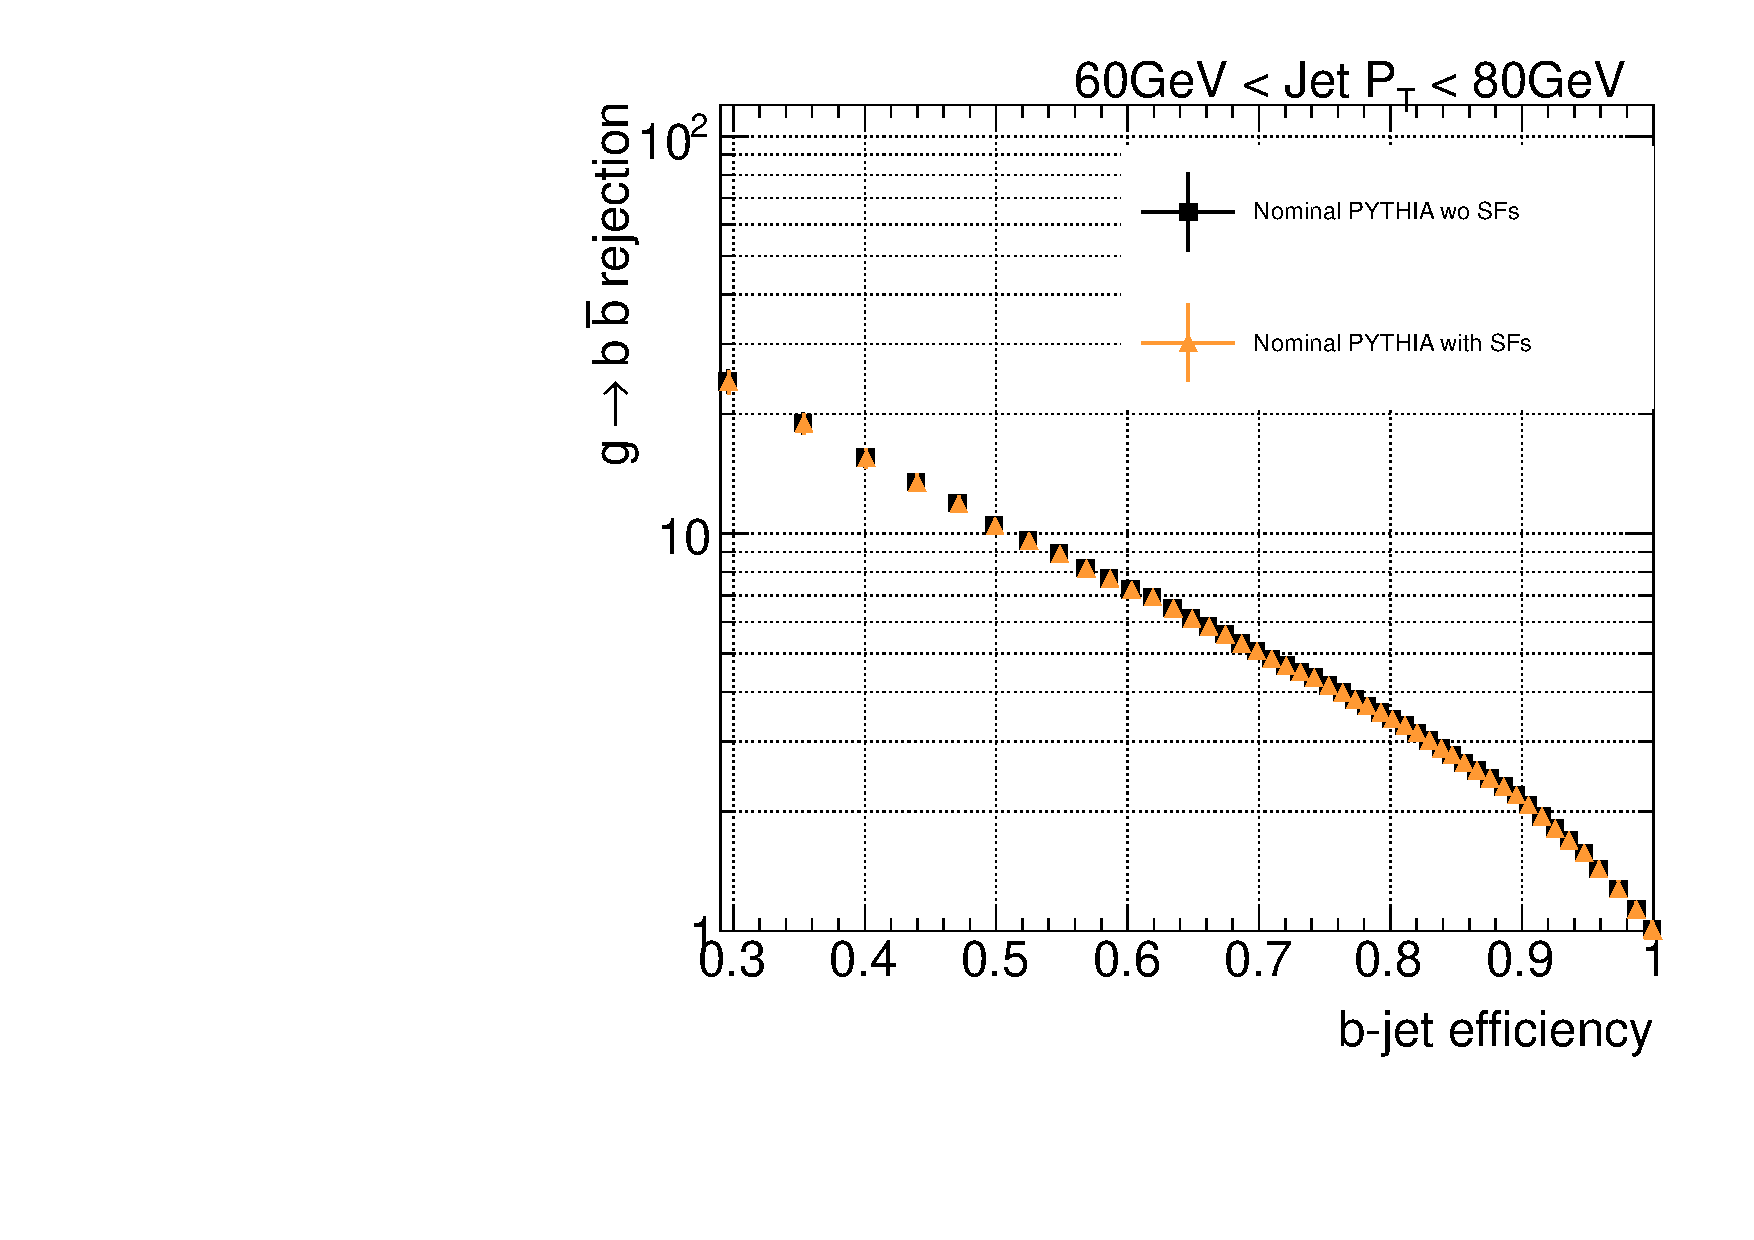
\includegraphics[width=0.49\textwidth]{FIGS/systematics/LlhoodKDE_ISO_BTagCalibTest_rejvseff060.pdf}
%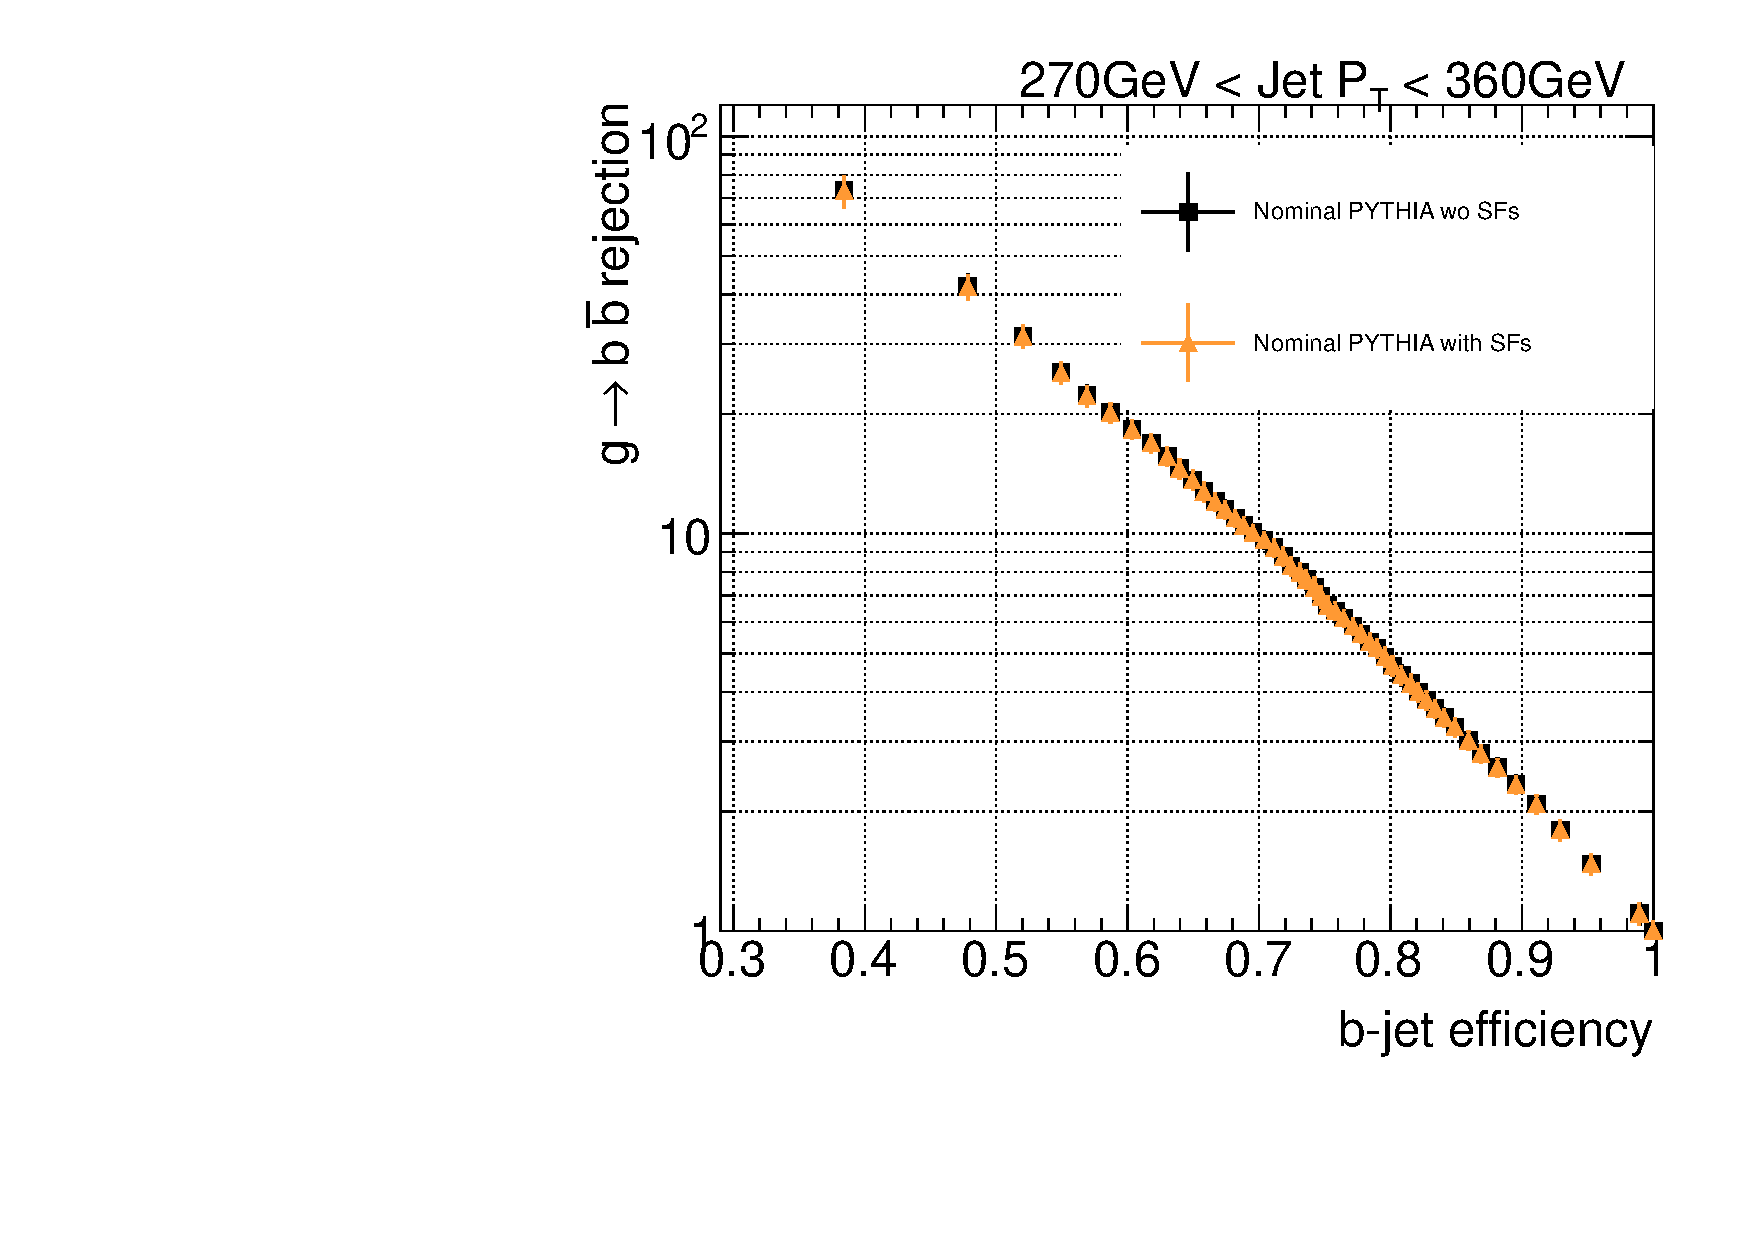
\includegraphics[width=0.49\textwidth]{FIGS/systematics/LlhoodKDE_ISO_BTagCalibTest_rejvseff270.pdf}
%\caption{Rejection of $g\rightarrow b \bar{b}$ merged b-jets as a function of $b$-jet efficiency with and without scale factors.}
%\label{fig:btaggingSFsPerf}
%\end{figure}

%

\vspace{3mm}
{ \em III. Track reconstruction efficiency}
\\[3mm]
This uncertainty arises from the limit of in the understanding of the material layout of the Inner Detector. To test its impact a fraction of tracks determined from the track efficiency uncertainty was randomly removed following the method in Ref.~\cite{JetMassNote}.%https://cdsweb.cern.ch/record/1344082?ln=en

The tracking efficiency systematics are given in bins of track $\eta$. For tracks with $p_{\rm{T}}^{\rm{track}} > 500$~MeV the uncertainties are independent of $\pt$:  2\% for $|\eta^{\rm{track}}|<1.3$, 3\% for $1.3<|\eta^{\rm{track}}|<1.9$, 4\% for $1.9<|\eta^{\rm{track}}|<2.1$, 4\% for $2.1<|\eta^{\rm{track}}|<2.3$ and 7\% for $2.3<|\eta^{\rm{track}}|<2.5$~\cite{chargemultiplicity}. All numbers are relative to the corresponding tracking efficiencies.  
%https://cdsweb.cern.ch/record/1286839
%http://arxiv.org/abs/1012.5104

The tracking variables were re-calculated and the performance of the nominal (pythia) likelihood was evaluated in the new sample with worse tracking efficiency. The rejection-efficiency plots, shown in Fig.~\ref{fig:trackefficiency}, show a small degradation of the performance which is comparable to the statistical uncertainty. The effect is however systematically present over all 16 \pt\ bin/working points, without a clear \pt\ dependence. We have thus taken the average over \pt, and obtained a global systematic uncertainty of 4\% both for the 50\% and 60\% efficiency working points.

\begin{figure}[tp]
\centering
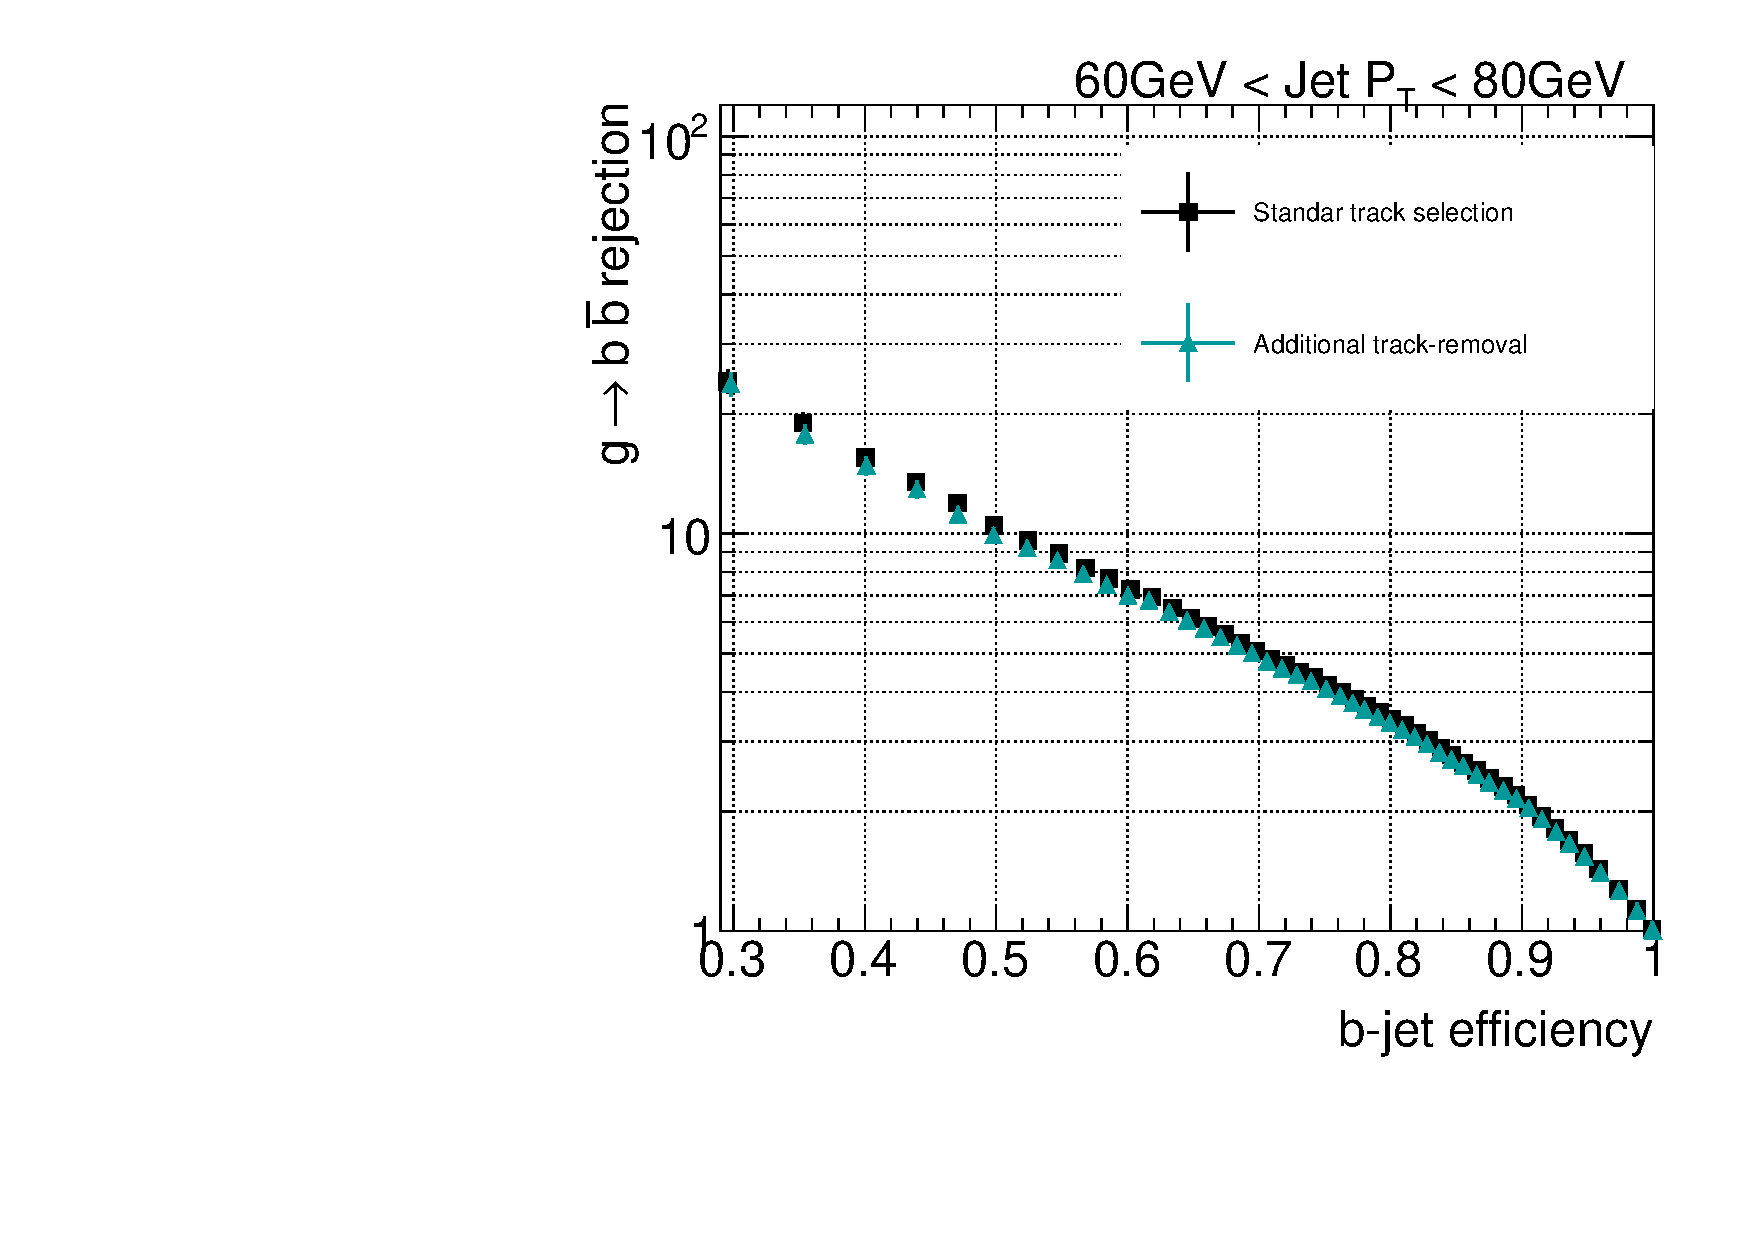
\includegraphics[width=0.49\textwidth]{FIGS/systematics/LlhoodKDE_ISO_TrackingUncertaintyTest_rejvseff060.pdf}
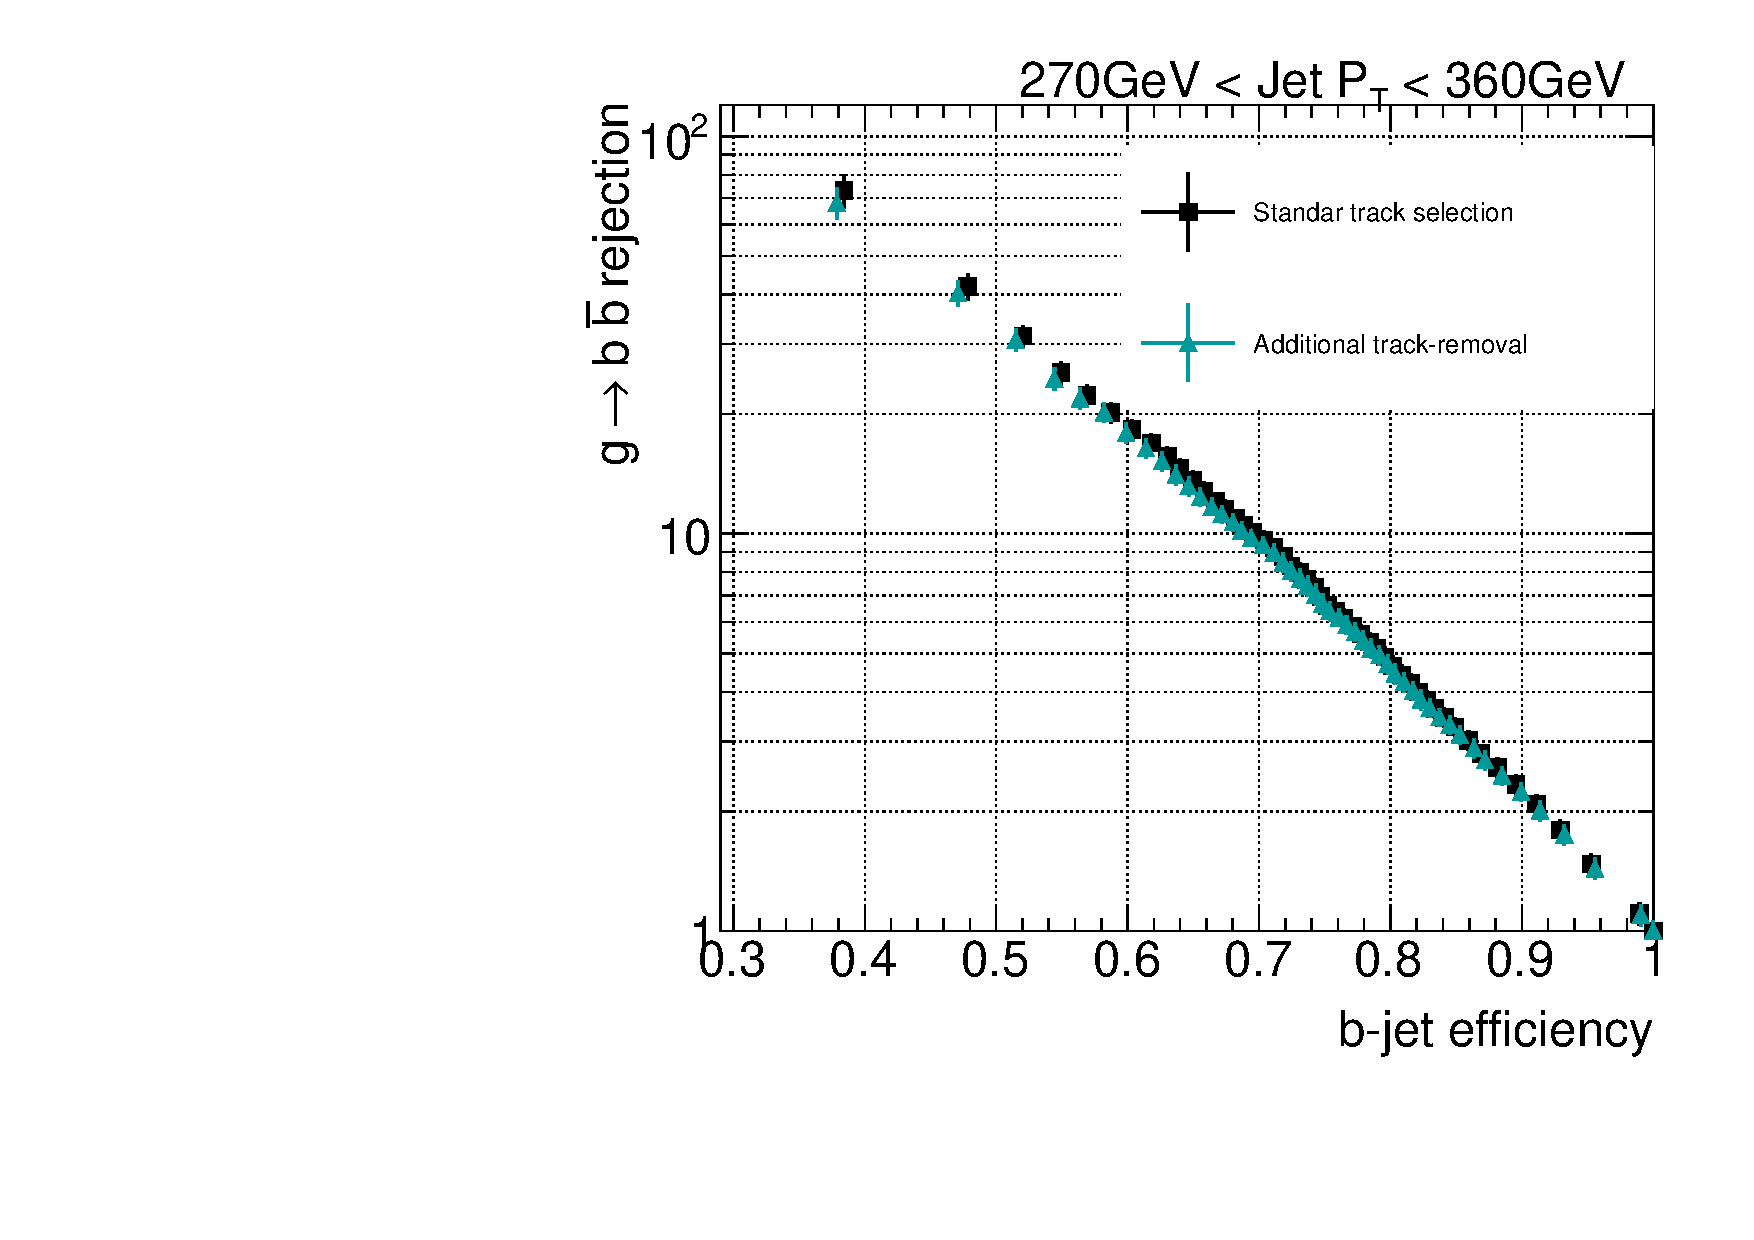
\includegraphics[width=0.49\textwidth]{FIGS/systematics/LlhoodKDE_ISO_TrackingUncertaintyTest_rejvseff270.pdf}
\caption{Rejection of $g\rightarrow b \bar{b}$ merged b-jets as a function of $b$-jet efficiency showing shift in likelihood performance caused by rejecting additional tracks.}
\label{fig:trackefficiency}
\end{figure}

\vspace{3mm}
{\em IV. Track momentum resolution}
\\[3mm]
The knowledge of the track momentum resolution is limited by the precision both in the material description of the Inner Detector and in the mapping of the magnetic field. Its uncertainty propagates to the kinematic variables used in the 
$g\rightarrow b \bar{b}$ tagger. In order to study this effect, track momenta are over-smeared according to the measured resolution uncertainties before computing the rejection. The actual smearing is done in 1/\pt, with an upper bound to the resolution uncertainty given by $\sigma(1/\pt)=0.02/\pt$~\cite{ATLAS-CONF-2010-009}. The effect is found to be negligible with respect to the statistical uncertainty.

\vspace{3mm}
{ \em V. Jet transverse momentum resolution}
\\[3mm]
The jet momentum resolution was measured for 2011 data and found to be in agreement with the predictions from the MC11 {\sc pythia8}-based simulation~\cite{JER2011}. The precision of this measurement, determined in $\pt$ and $\eta$ bins, and, is typically 10\%.
The systematic uncertainty due to the calorimeter jet $\pt$ resolution was estimated by over-smearing the jet $4$-momentum in the simulated data, without changing jet $\eta$ or $\phi$ angles. The performance is found to globally decrease by 6\%, without a particular \pt\ dependence.

%\begin{figure}[tp]
%\centering
%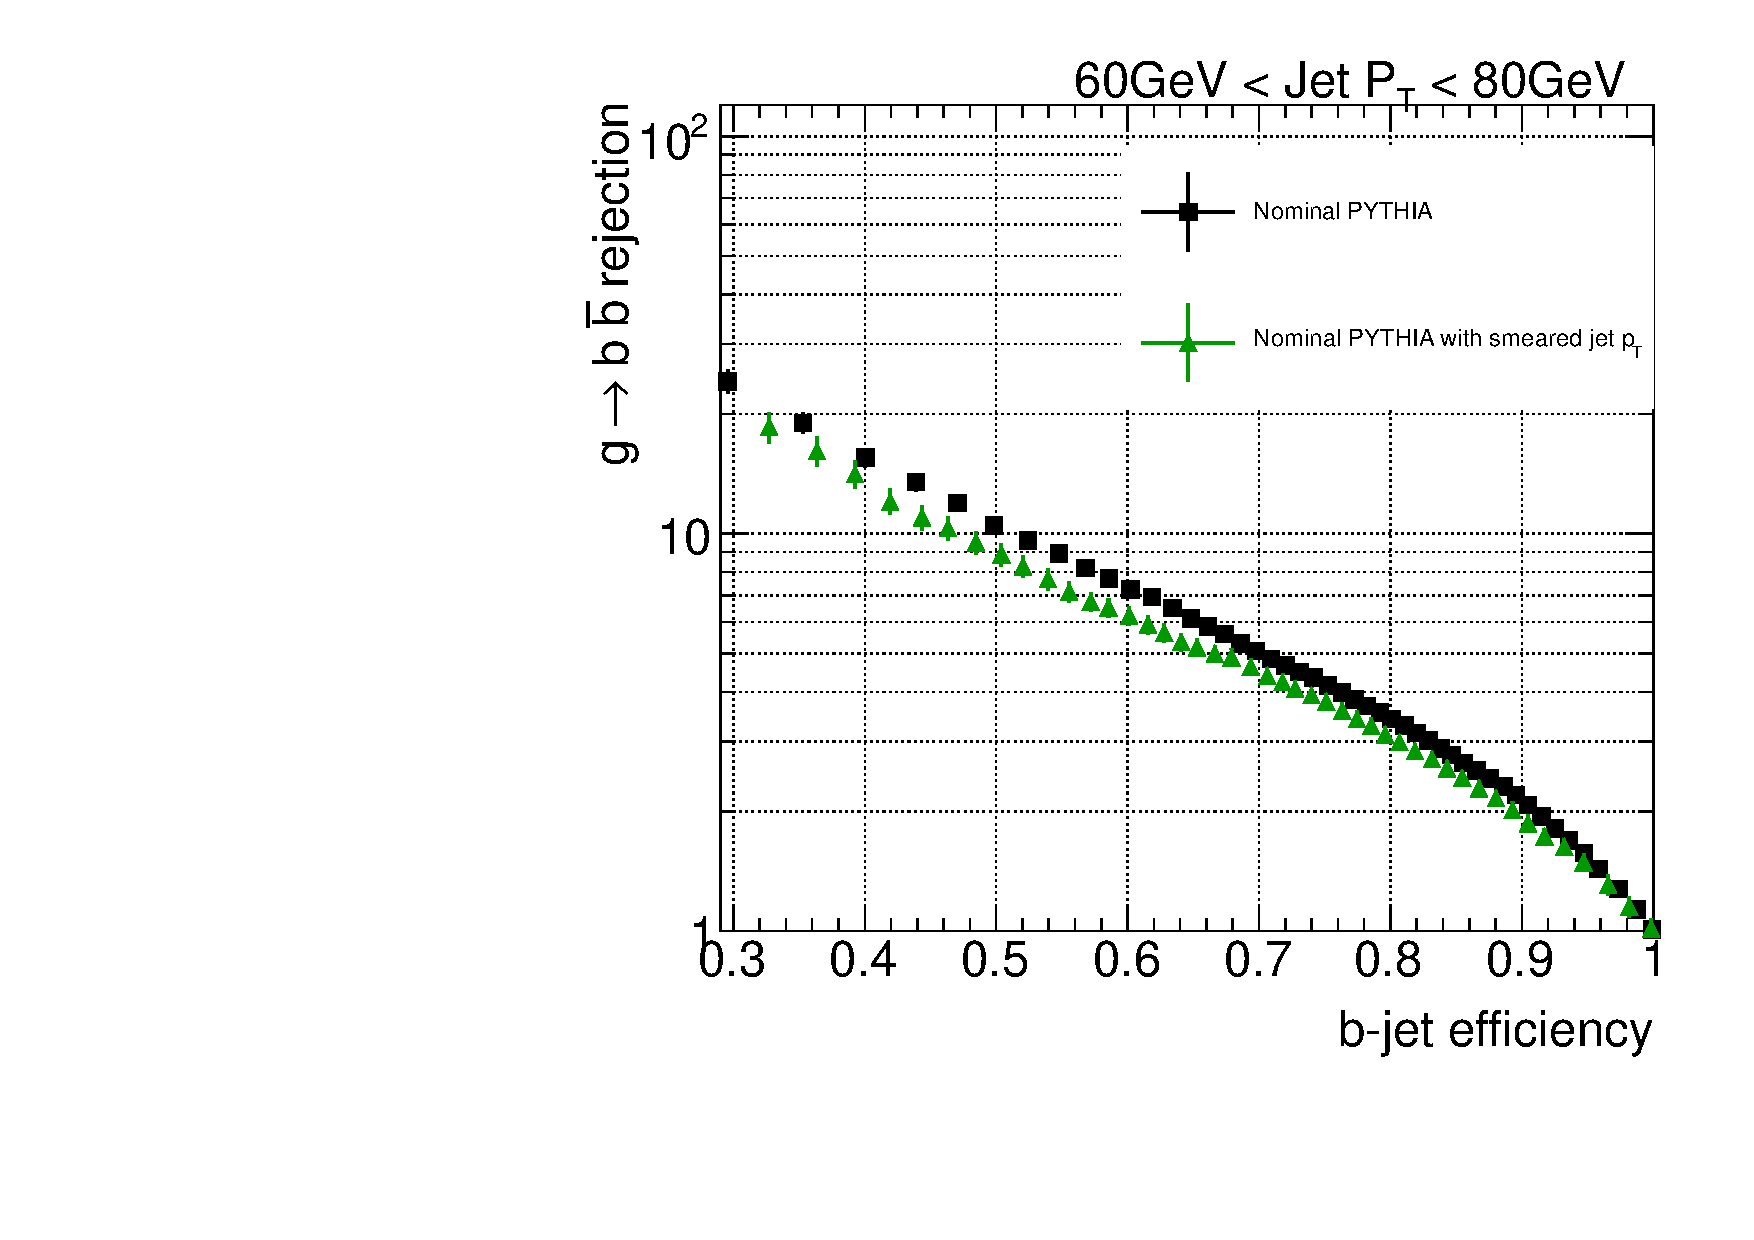
\includegraphics[width=0.49\textwidth]{FIGS/systematics/LlhoodKDE_ISO_SmearedJetPtTest_rejvseff060.pdf}
%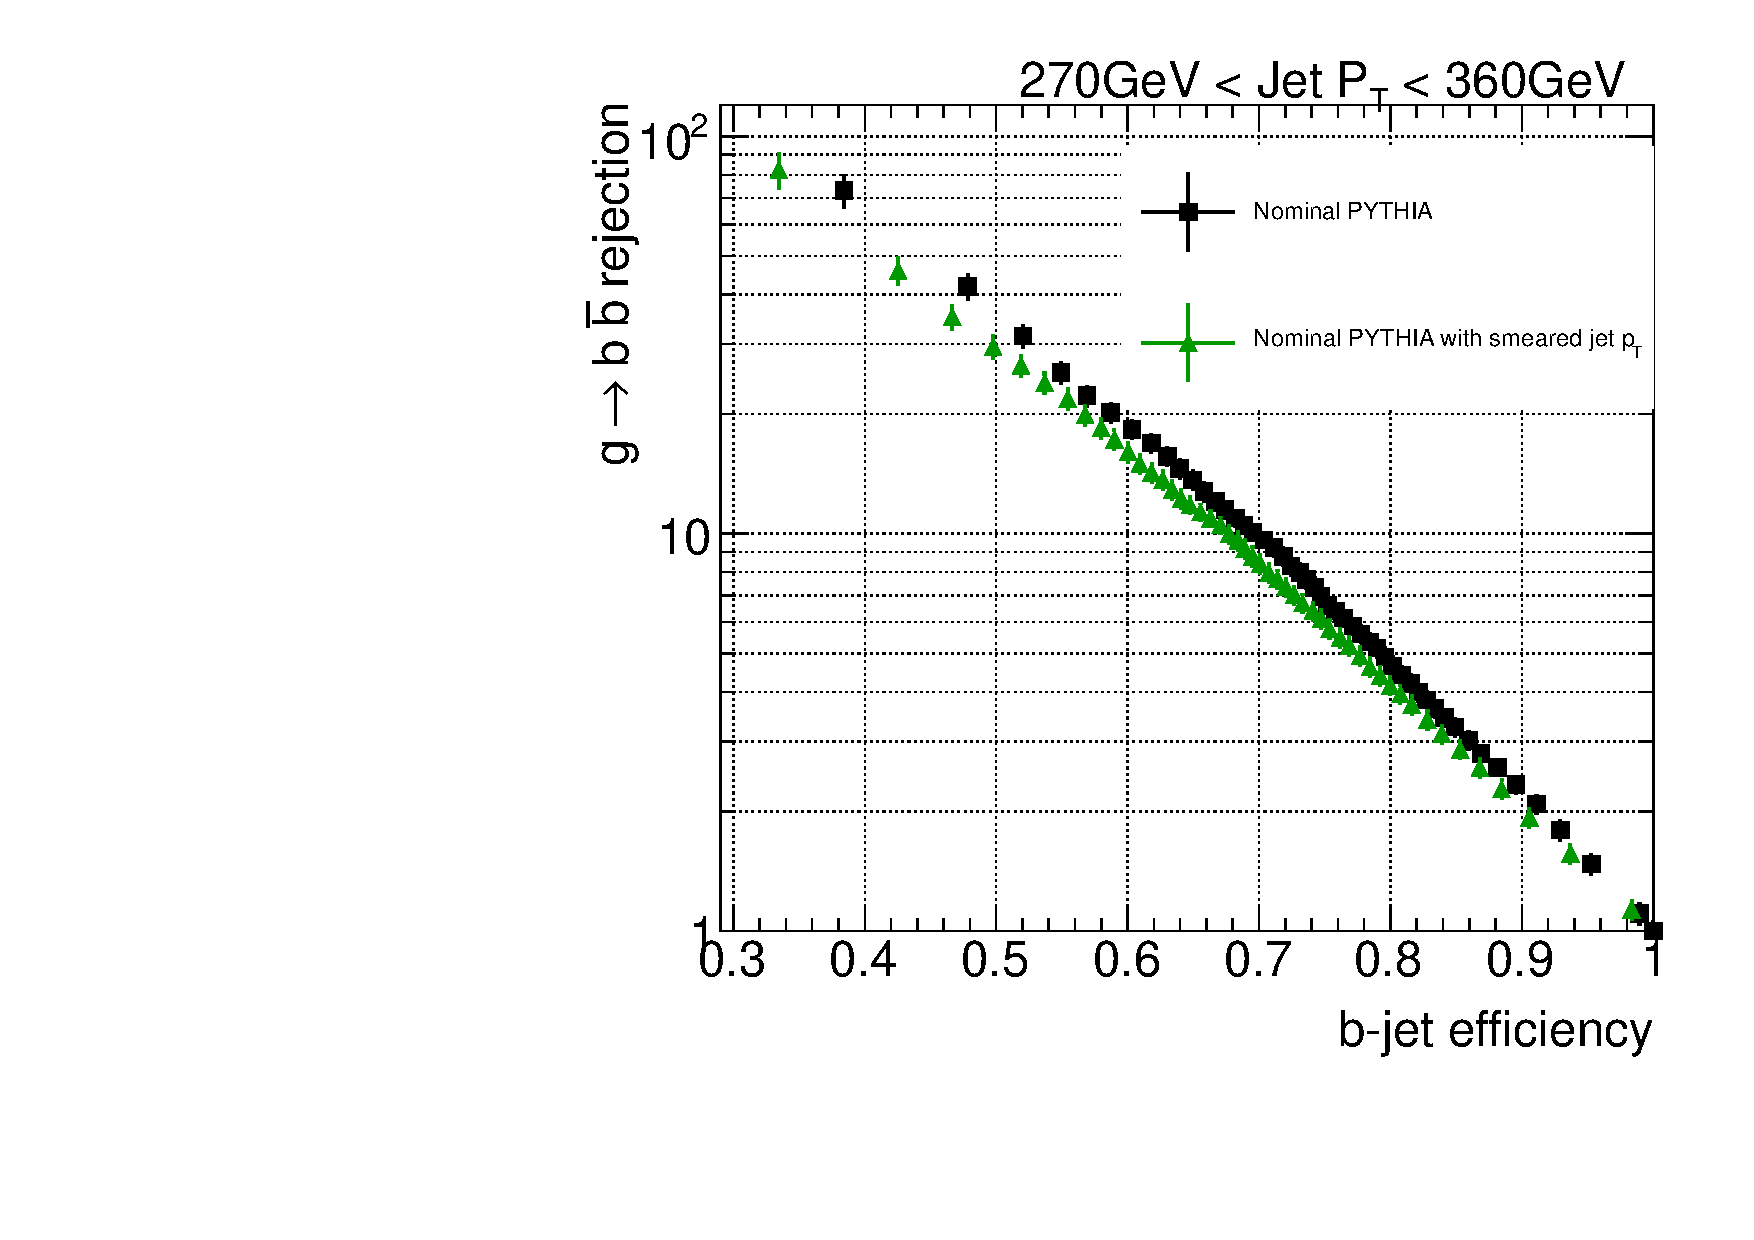
\includegraphics[width=0.49\textwidth]{FIGS/systematics/LlhoodKDE_ISO_SmearedJetPtTest_rejvseff270.pdf}
%\caption{Rejection of $g\rightarrow b \bar{b}$ merged b-jets as a function of $b$-jet efficiency for jets with smeared $\pt$.}
%\label{fig:jetresolution}
%\end{figure}
\vspace{3mm}
The different contributions to the systematic uncertainty on the $g\rightarrow b \bar{b}$ rejection are summarized in Table~\ref{tb:systematics}.

%\begin{table}[!hbt] %[h]
%\renewcommand{\arraystretch}{1.2}
%\centering
%\begin{tabular}{ | c | c |}
%\hline
%  Systematic source &~~Uncertainty~~\\ \hline
%   pile-up          &  neglible     \\ 
%   $b$-tag eff.     &  neglible     \\ 
%   track reco eff.  &    4\%        \\ 
%   track \pt\ resol.&  neglible     \\
%   jet \pt\ resol.  &    6\%        \\ \hline 
%\end{tabular}
%\caption{Systematic uncertainities in the merged $b$-jet rejection (common to both the 50\% and the 60\% efficiency working points).}
%\label{tb:systematics}
%\end{table}



%------------------------------------------------------------------------
\section{Other Monte Carlo generators}\label{sec:otherMC}
%------------------------------------------------------------------------
%{\em Uncertainties due to the event modelling in the Monte Carlo generators}

The development, training and performance determination of the tagger has been done using Monte Carlo events generated with the {\sc pythia8} event simulator, interfaced to the {\sc geant4} based simulation of the ATLAS detector. An immediate question is what the performance would be if studied with a different simulation. In this section we investigate this question for the Perugia tune of {\sc pythia8} and the {\sc herwig++} event generators.

Fig.~\ref{fig:performanceotherMC} shows a comparison of the performance-efficiency plots between nominal {\sc pythia} and the alternative simulations for four selected \pt\ bins covering the full kinematic range. The larger errors are due to the reduced statistics available, which are even lower for the Perugia case than for {\sc herwig}.


%In order to account for the dependence on different generator models and tunes the likelihood performance was tested using other Monte Carlo simulations. Results with nominal Pythia were compared to the performance derived with dijet samples generated with Herwig++ and with the Perugia tune of Pythia. The comparison can be seen in Fig.~\ref{fig:performanceotherMC}. 

The performance in {\sc herwig} shows a systematic trend, with agreement at low \pt\ and increasingly poor performances compared to {\sc pythia} as \pt\ grows. For the Perugia tune, on the other hand, there is no definite behavior, with the performance fluctuating above or below the nominal simulation for different \pt\ bins consistently with the statistical uncertainties.

The reason for the systematic difference observed between the performances of {\sc pythia} and {\sc herwig} can be traced to the extent with which jets are accurately modelled. Fig.~\ref{fig:herwigdatamc} compares the measured jet track multiplicity distributions in $b$-tagged jets and the prediction from both simulations. It is observed that indeed {\sc herwig++} does not correctly reproduce the data, particularly at medium and high \pt. Although not shown, the level of agreement is found to be better for jet-track width and the angle between the leading subjets, the two other variables used for discrimination.



%the comparion between jet distribution in experimental data and  Herwig++ Monte Carlo events was performed for $b$-tagged jets. The results for the jet track-multiplicity can be seen in Fig.~\ref{fig:herwigdatamc}. We find that Herwig++ does not reproduce data jet distributions correctly at medium and high \pt.



\begin{figure}[tp]
\centering
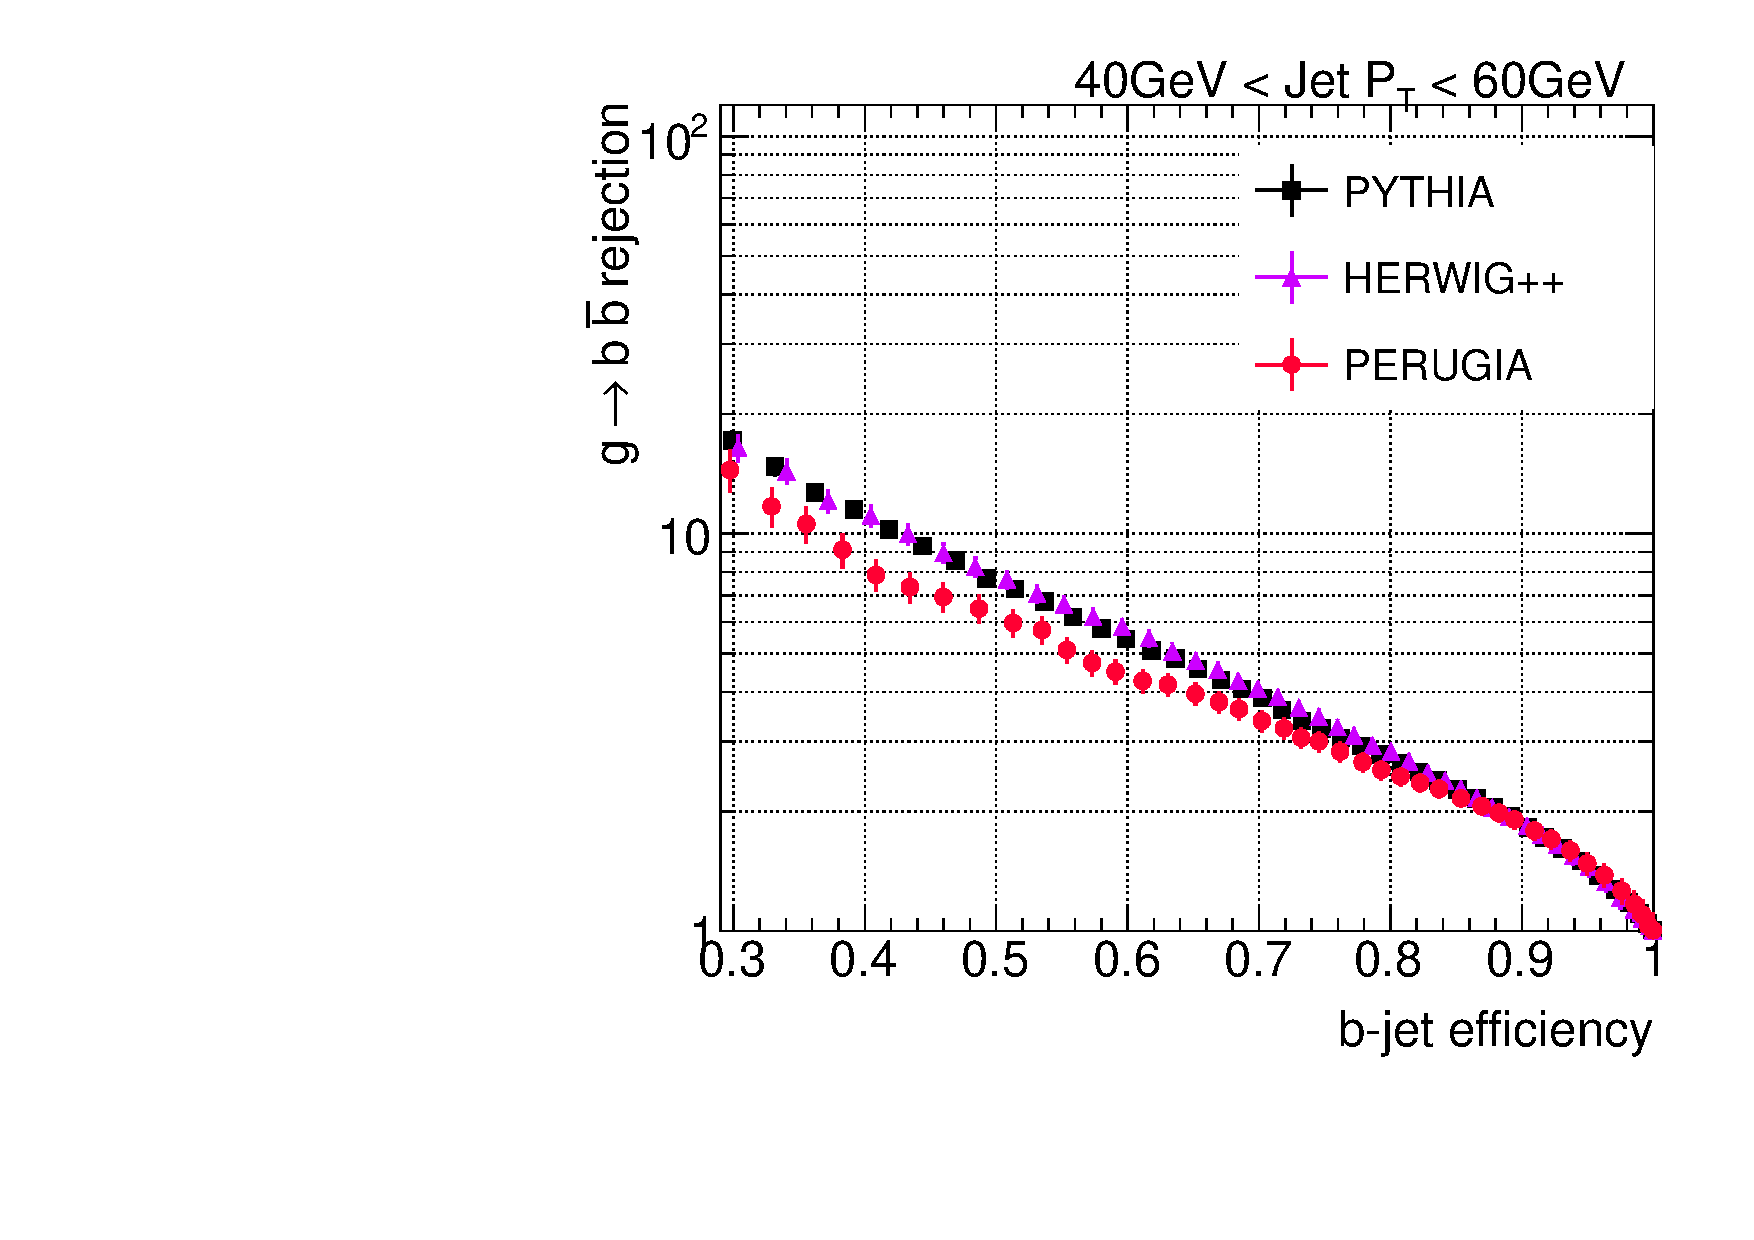
\includegraphics[width=0.49\textwidth]{FIGS/systematics/newInterpLlhoodKDE_ISO_DiffMCGen_rejvseff040.pdf}
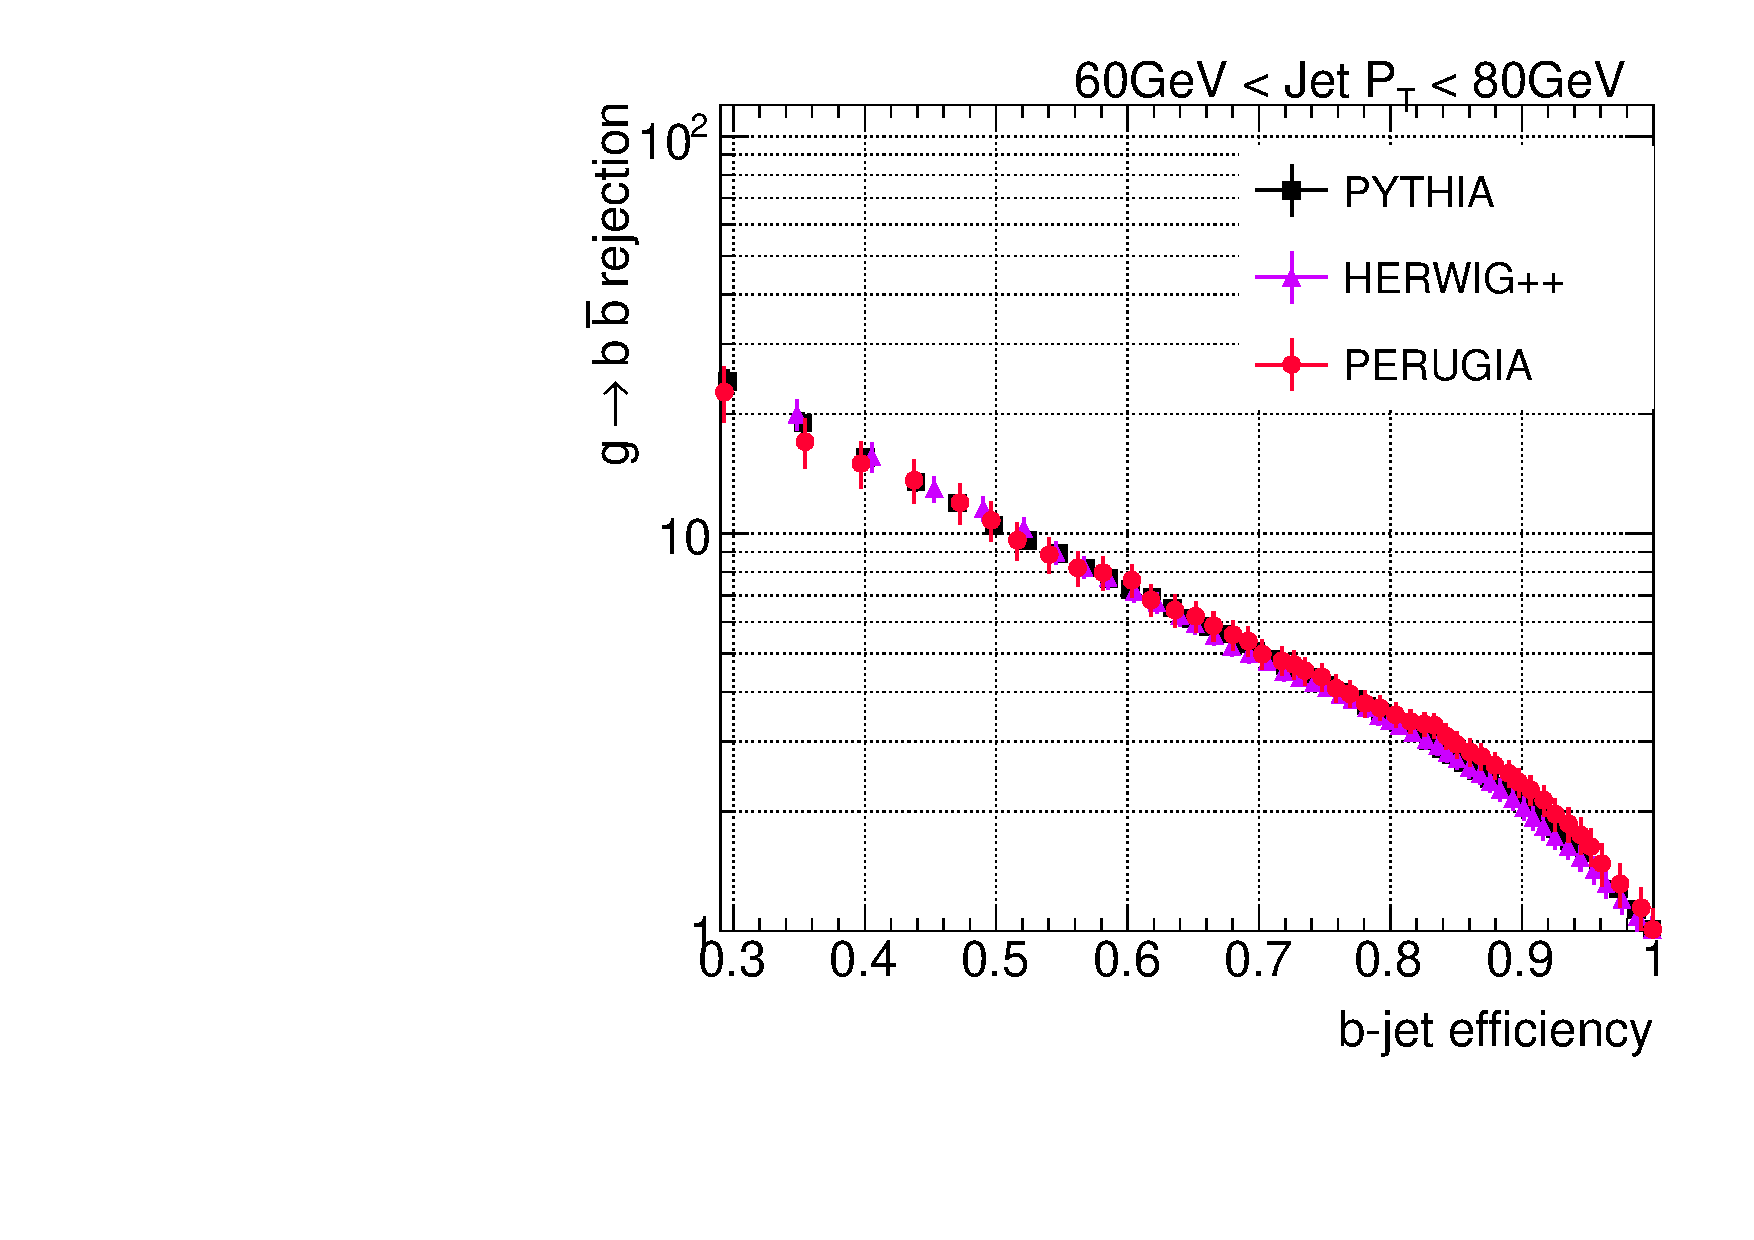
\includegraphics[width=0.49\textwidth]{FIGS/systematics/newInterpLlhoodKDE_ISO_DiffMCGen_rejvseff060.pdf}
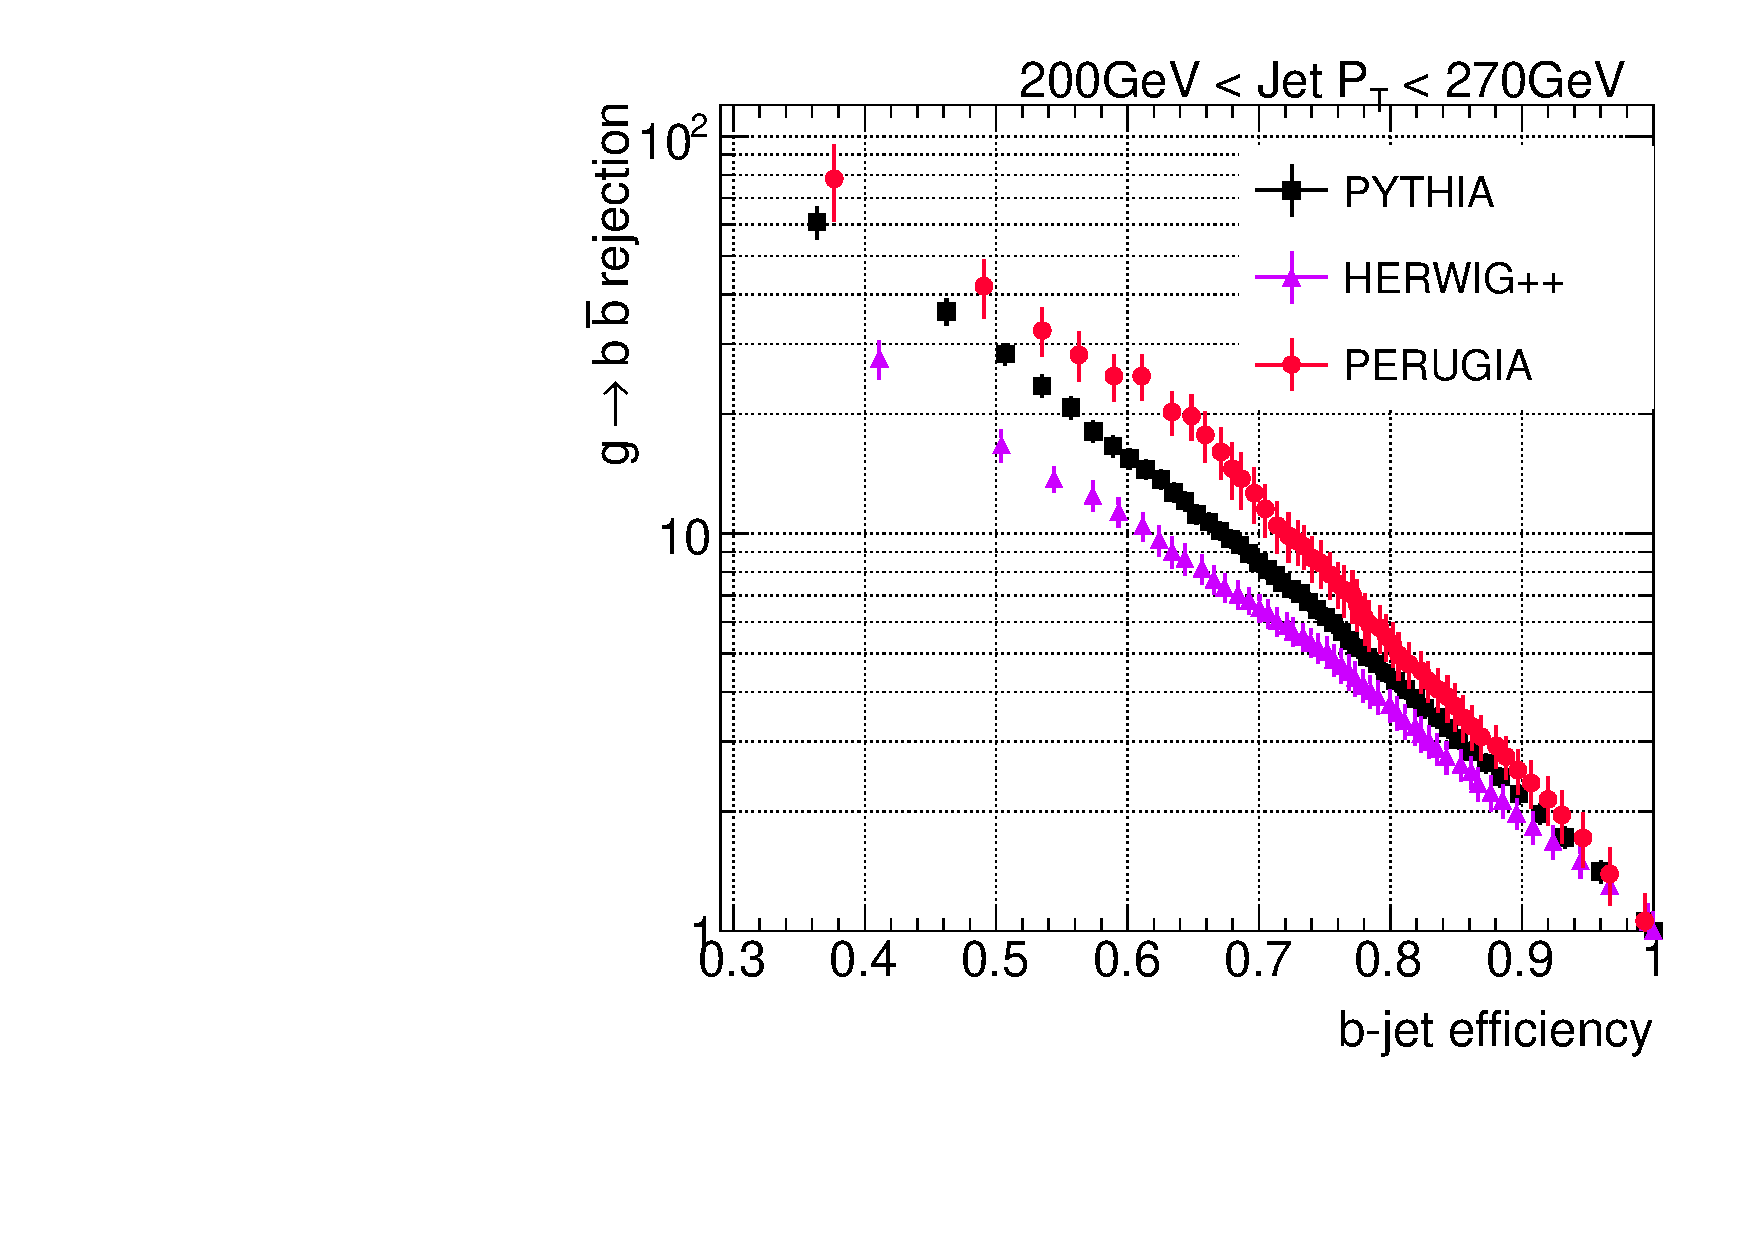
\includegraphics[width=0.49\textwidth]{FIGS/systematics/newInterpLlhoodKDE_ISO_DiffMCGen_rejvseff200.pdf}
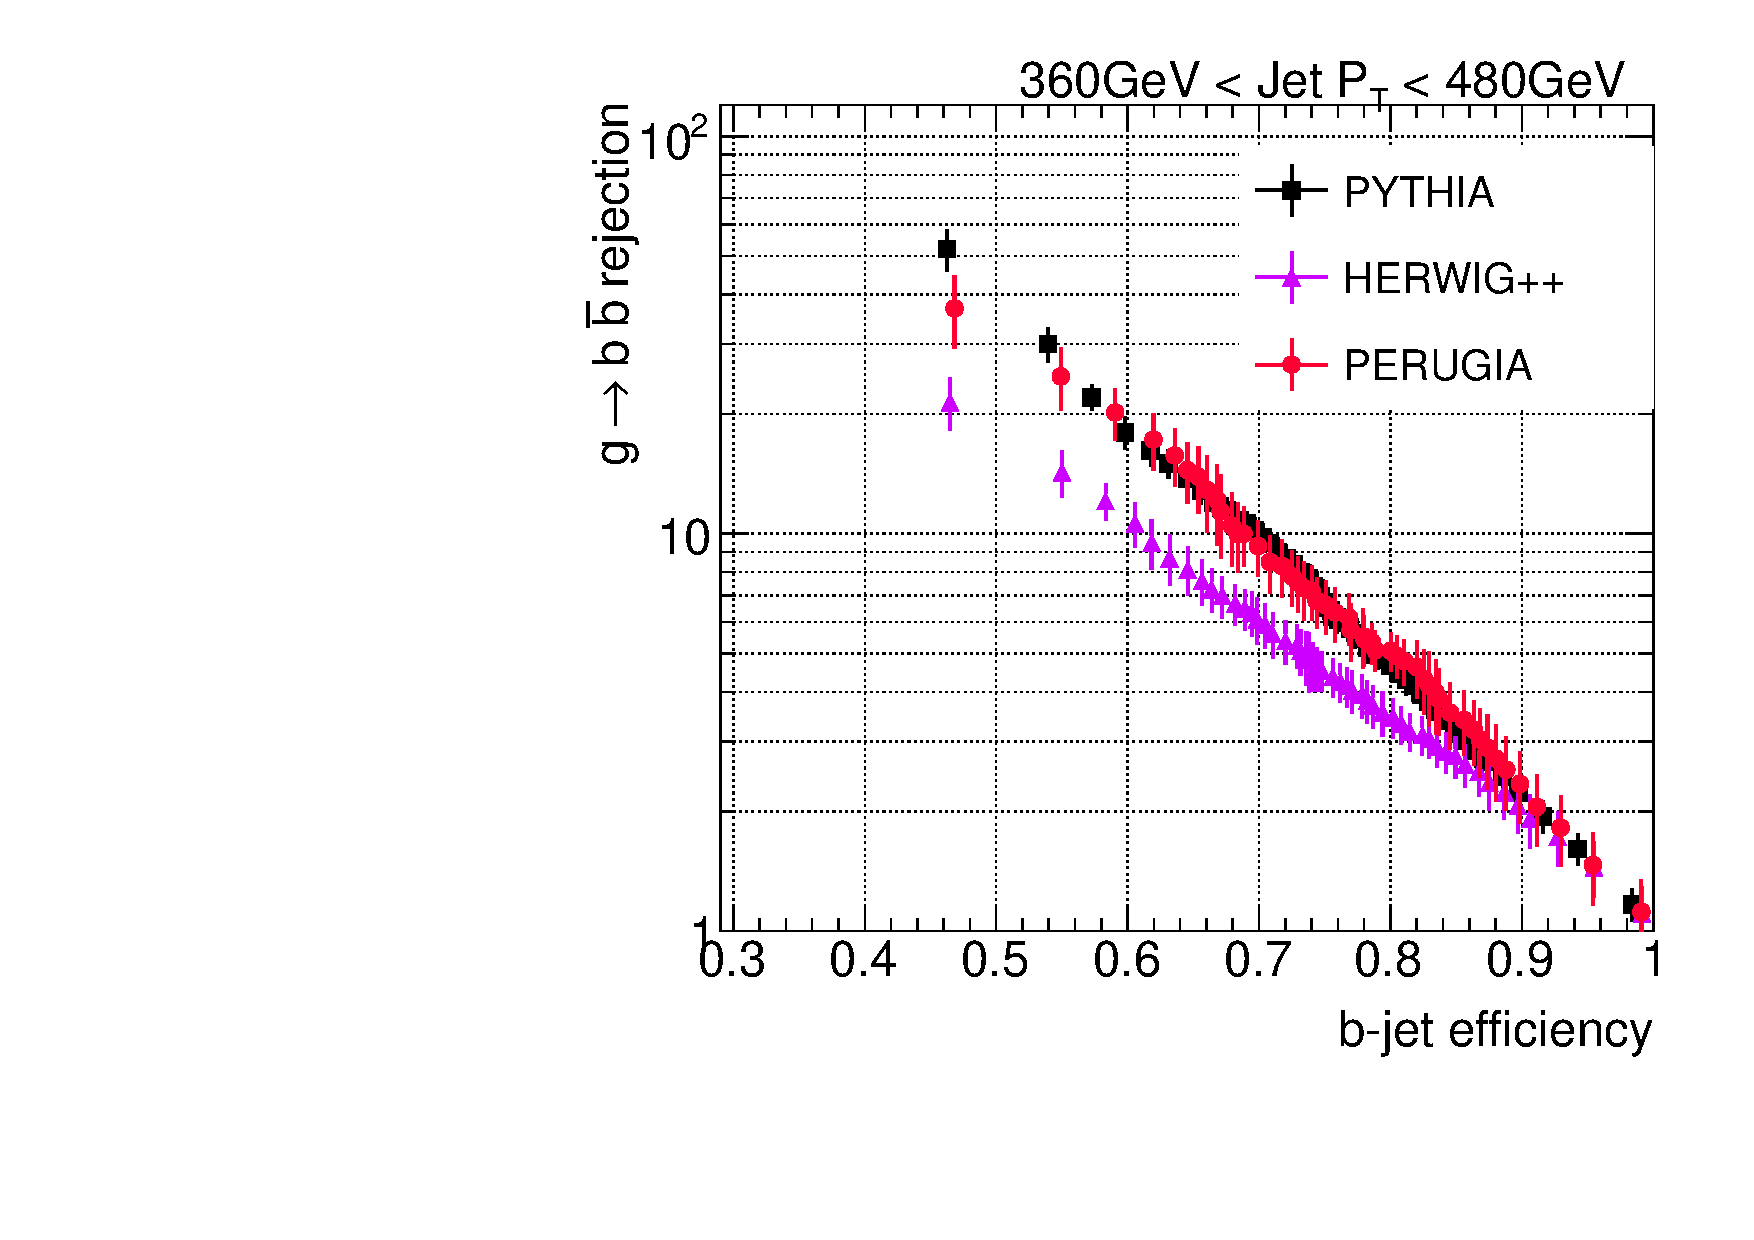
\includegraphics[width=0.49\textwidth]{FIGS/systematics/newInterpLlhoodKDE_ISO_DiffMCGen_rejvseff360.pdf}
\caption{Rejection of $g\rightarrow b \bar{b}$ merged b-jets as a function of single $b$-jet identification efficiency for different Monte Carlo generators.}
\label{fig:performanceotherMC}
\end{figure}

\begin{figure}[tp]
\centering
\includegraphics[width=0.49\textwidth]{FIGS/systematics/DataVarNtrkPT040.pdf}
\includegraphics[width=0.49\textwidth]{FIGS/systematics/DataVarNtrkPT200.pdf}
\caption{Distribution of the jet track-multiplicity in 2 different jet $\pt$ bins, for experimental data from data-taking periods B to H (solid black points) and Herwig++ events (solid violet triangules). The ratio datab\/Herwig++ simulation is shown at the bottom of the plot. Pythia distribution is also shown for reference.}
\label{fig:herwigdatamc}
\end{figure}


%
%%%%%%%%%%%%%%%%%%%%%%%%%%%%%%%%%%%%%%%%%%%%%%%%%%%%%%%%%%%%%%%%%%%%%%%%%%%%%%%
% Fractio of gluon splitting in data
%%%%%%%%%%%%%%%%%%%%%%%%%%%%%%%%%%%%%%%%%%%%%%%%%%%%%%%%%%%%%%%%%%%%%%%%%%%%%%%
%
\chapter{Fraction of gluon-splitting jets in data}

%------------------------------------------------------------------------
\section{Template fits}\label{sec:FractionSystematics}
%------------------------------------------------------------------------

%------------------------------------------------------------------------
\section{Systematic uncertainties}\label{sec:FractionSystematics}
%------------------------------------------------------------------------
